% **************************************************
% Macro specifiche per il documento corrente
% **************************************************
% Nome
\newcommand{\docName}{Piano di Qualifica}
% Nome file
\newcommand{\docFileName}{piano\_di\_qualifica.4.0.pdf}
% Versione
\newcommand{\docVers}{4.0}
% Data creazione
\newcommand{\creationDate}{2012-12-10}
% Data ultima modifica
\newcommand{\modificationDate}{2013-05-17}
% Stato in {Approvato, Non approvato}
\newcommand{\docState}{Approvato}
% Uso in {Interno, Esterno}
\newcommand{\docUsage}{Esterno}
% Destinatari da specificare come nome1\\ &nome2\\ ecc.
\newcommand{\docDistributionList}{Prof. Tullio Vardanega\\ & Prof. Riccardo Cardin \\& Dott. Gregorio Piccoli}
% Redattori da specificare come nome1\\ &nome2\\ ecc.
\newcommand{\docAuthors}{Stefano Farronato\\ &Elena Zecchinato}
% Approvato da
\newcommand{\approvedBy}{Marco Schivo}
% Verificatori
\newcommand{\verifiedBy}{Diego Beraldin}
% Perscorso (relativo o assoluto) che punta alla directory contenente shared/
% come sua sottodirectory (per comodità chiamiamola 'doc root').
\newcommand{\docRoot}{..}
% definire se si vuole l'indice delle tabelle
\def\INDICETABELLE{false}
% definire se si vuole l'indice delle figure
\def\INDICEFIGURE{false}

% importa il preambolo condiviso da tutti i documenti
% shared/preamble.tex
%
% Questo documento contiene la parte del preambolo condivisa e viene pertanto
% richiamato nel 'master' di tutti i documenti di progetto.  Al suo interno
% contiene le inclusioni (e le configurazioni) di tutti i package richiesti per
% la compilazione dei documenti, le macro di carattere generale e la definizione
% degli stili di pagina.

\documentclass[a4paper,10pt,openright]{article}

% **************************************************
% Macro generiche
% **************************************************
\newcommand{\team}{Software Synthesis}                    % chi siamo
\newcommand{\email}{software.synthesis@gmail.com}         % e-mail
\newcommand{\caName}{}                                    % titolo capitolato
\newcommand{\caDescr}{}                                   % descrizione
\newcommand{\inglese}[1]{\textit{#1}}

% **************************************************
% Codifica e lingua dei documenti
% **************************************************
\usepackage[utf8x]{inputenc}                              % codifica caratteri dei documenti sorgenti
\usepackage[english,italian]{babel}                       % localizzazione ai fini di sillabazione e cross-references
\usepackage[T1]{fontenc}                                  % codifica font di output

% **************************************************
% Definizione geometria della pagina
% **************************************************
\usepackage[a4paper,head=4cm,top=4.5cm,bottom=3cm,left=3cm,right=3cm,bindingoffset=5mm]{geometry}

% *************************************************
% Intestazioni e piè di pagina personalizzati
% *************************************************
\usepackage{fancyhdr}
% stile normale
\fancypagestyle{normal}{
\fancyhead{}                                              % intestazione
\fancyhead[RE,RO]{
\begin{picture}(0,0)
  \put(-410,0){
\includegraphics[width=1.02\textwidth]{header_logo}}
  \put(-410,10){\sffamily\large\leftmark}
\end{picture}
\vspace{-4pt}
}
\renewcommand{\headrulewidth}{.4pt}                       % riga sotto l'intestazione
\cfoot{}                                                  % piè di pagina
\fancyfoot[RO,LE]{\sffamily
  pag.~\thepage{} di \pageref{LastPage}}                  % a dx nelle pag. dispari e a sx in quelle pari
\fancyfoot[RE,LO]{\sffamily\docFileName{} -- v.\docVers}
\renewcommand{\footrulewidth}{.4pt}                       % riga sopra il piè di pagina
}
% stile per gli indici
\fancypagestyle{toc}{
\fancyhead{}                                              % intestazione
\fancyhead[RE,RO]{
\begin{picture}(0,0)
  \put(-410,0){
\includegraphics[width=1.02\textwidth]{header_logo}}
\end{picture}
}
\renewcommand{\headrule}{}                                % nessuna riga sotto l'intestazione
\cfoot{}                                                  % piè di pagina
\fancyfoot[RO,LE]{\sffamily\thepage{}}                    % a dx nelle pag. dispari e a sx in quelle pari
\fancyfoot[RE,LO]{\sffamily\docFileName{} -- v.\docVers}
\renewcommand{\footrulewidth}{.4pt}                       % riga sopra il piè di pagina
}

\pagestyle{fancy}                                         % premetto: non so usare bene le marche:
\renewcommand{\sectionmark}[1]{\markboth{#1}{#1}}         % se qualcuno ha idee migliori si faccia avanti!

% **************************************************
% Tabelle
% **************************************************
\usepackage{tabularx}                                     % tabelle di larghezza fissa con una o più colonne variabili
\usepackage{multirow}                                     % colonne con colonne che si estendono per più righe
\usepackage{booktabs}                                     % per inserire l'ambiente table e le righe orizz. nelle tabelle
\usepackage{longtable}			                          % tabelle oltre i limiti di pagina

% **************************************************
% Cross-references e collegamenti ipertestuali
% **************************************************
\usepackage[hidelinks]{hyperref}
\hypersetup{%
  colorlinks=false, linktocpage=false, pdfborder={0,0,0}, pdfstartpage=3, pdfstartview=FitV,%
  urlcolor=Cyan, linkcolor=Cyan, citecolor=Black, %pagecolor=Black,%
  pdftitle={\docName}, pdfauthor={\team}, pdfsubject={}, pdfkeywords={},%
  pdfcreator={pdflatex}, pdfproducer={pdflatex with hyperref package}%
}

% **************************************************
% Immagini e grafica
% **************************************************
\usepackage{graphicx}                                     % supporto ad aspetti avanzati delle immagini
\graphicspath{{\docRoot/pics/}}                           % percorso contenente tutti i file immagini
\usepackage{color}                                        % permette di colorare facilmente il testo

% **************************************************
% Altri pacchetti opzionali
% **************************************************     
\usepackage{lastpage}                                     % per sapere il numero totale di pagine
\usepackage{lipsum}                                       % genera "dummy text" per prove di impaginazione
\usepackage{eurosym}                                      % per il simbolo dell'euro usare \EUR{x} dove x è l'importo


% pacchetto per caratteri esotici
\usepackage{pifont}
\newcommand{\passed}{\ding{52}{ }}
\newcommand{\failed}{\ding{56}{ }}

% per le appendici
\renewcommand{\appendixname}{Appendici}

% Fine del preambolo e inizio del documento
\begin{document}

% Inclusione della prima pagina
% shared/firstpage.tex
%
% Questo documento definisce il contenuto della prima pagina, che si suppone
% essere uguale in tutti i documenti.  Oltre al logo e al titolo, la prima
% pagina contiene i metadati relativi al documento in cui viene inclusa.


% rimuove intestazioni e piè di pagina
\pagestyle{empty}

\begin{center}

% logo del gruppo

\includegraphics[width=1.5\textwidth]{logo}

\vspace{1in}

% titolo del documento
{\Huge\bfseries \docName}

\vspace{1in}

% tabella riepilogativa
\begin{tabularx}{.7\textwidth}{>{\bfseries\sffamily}l>{\sffamily}l}
\toprule
\multicolumn{2}{>{\sffamily}c}{Informazioni sul documento}\\
\midrule
Nome file:            & \docFileName\\
Versione:             & \docVers\\
Data creazione:       & \creationDate\\
Data ultima modifica: & \modificationDate\\
Stato:                & \docState\\
Uso:                  & \docUsage\\
Redattori:            & \docAuthors\\
Approvato da:         & \approvedBy\\
Verificatori:         & \verifiedBy\\
\bottomrule
\end{tabularx}

\end{center}

\newpage


% Storico delle modifiche
\section*{Storia delle modifiche}
\begin{longtable}{lp{.3\textwidth}lll}
\toprule
Versione & Descrizione intervento & Redattore & Ruolo & Data\\
\midrule % inserire qui il contenuto della tabella



4.0 & Approvazione documento& Marco Schivo &Responsabile & 2013-05-17\\
3.6 &  Verifica del documento &Diego Beraldin &Verificatore & 2013-05-16\\
3.5 & Considerazioni finali sui test e integrazione dati sulle metriche, creata e documentata la sezione relativa ai test di sistema & Stefano Farronato &Verificatore & 2013-05-15\\
3.4 & Documentati ulteriori test sul Presenter e create relative tabelle di tracciamento & Elena Zecchinato &Verificatore & 2013-05-13\\
3.3 & Documentati ulteriori test sul Model e create relative tabelle di tracciamento& Stefano Farronato &Verificatore & 2013-05-13\\
3.2 & Implementati in appendice sezioni relative alle considerazioni per il miglioramento, resoconto attività di verifica ed esiti delle revisioni& Elena Zecchinato &Verificatore & 2013-05-10\\
3.1 & Integrata in appendice il documento in precedenza separato sui test & Stefano Farronato &Verificatore & 2013-05-09\\
3.0 & Approvazione documento& Diego Beraldin &Responsabile & 2013-03-16\\
2.8 & Correzione errori riscontrati in fase di verifica& Stefano Farronato &Progettista & 2013-03-16\\
2.8 & Verifica lessico ortografica del documenti& Riccardo Tresoldi &Progettista & 2013-02-16\\
2.7 & Aggiornata sezione ``Dettaglio dell'esito delle revisioni'' e ``Appendice'' & Elena Zecchinato &Progettista & 2013-03-16\\
2.6 & Aggiornata sezione ``Dettaglio dell'esito delle revisioni'' e ``Appendice'' & Elena Zecchinato &Progettista & 2013-03-15\\
2.5 & Aggiunta sezione ``Autovalutazione'' & Andrea Rizzi &Progettista & 2013-03-15\\
2.4 & Aggiornate e corrette definizioni analisi statica e dinamica & Stefano Farronato &Progettista  & 2013-03-15\\
2.3 & Riscritta sottosezione ``Metriche''  & Stefano Farronato &Progettista  & 2013-03-14\\
2.2 & Corretta sezione ``Metriche e metodi'' in ``Tecniche, metodi e metriche'' & Elena Zecchinato &Progettista & 2013-03-14\\
2.1 & Corretta sezione ``Qualità di processo'' & Stefano Farronato &Progettista & 2013-03-14\\
2.0 & Approvazione del documento& Andrea Meneghinello &Responsabile & 2013-01-19\\
1.8 & Verifica finale del documento& Andrea Rizzi &Verificatore & 2013-01-18\\
1.7 & Correzione errori riscontrati in fase di verifica& Riccardo Tresoldi &Progettista & 2013-01-18\\
1.6 & Verifica lessico ortografica del documento& Elena Zecchinato &Verificatore & 2013-01-18\\
1.5 & Aggiornamento capitolo ``Prossima versione piano di qualifica'' e riscritta sezione ``software''& Stefano Farronato &Progettista & 2013-01-17\\
1.4 & Creazione e organizzazione capitolo ``Appendice'' e sezioni interne &Riccardo Tresoldi &Progettista & 2013-01-16\\
1.3 & Correzione capitolo riguardante ``Misure, Metriche e metodi'' &Riccardo Tresoldi &Progettista & 2013-01-15\\
1.3 & Stesura capitolo ``Resoconto esito delle revisioni'' e sezioni interne &Riccardo Tresoldi &Progettista & 2013-01-14\\
1.2 & Correzione capitolo ``Visione generale strategia di verifica'' modificando strutturalmente la parte relativa a ``Organizzazione, pianificazione strategica, pianificazione temporale e responsabilità''&Stefano Farronato &Progettista & 2013-01-14\\
1.1 & Stesura sezione ``qualità di processo'' & Stefano Farronato &Progettista & 2013-01-13\\

1.0 & Approvazione documento & Elena Zecchinato & Responsabile & 2012-12-18\\
0.12 & Correzione errori segnalati dal verificatore & Stefano Farronato & Analista & 2012-12-18\\
0.11 & Verifica Capitoli 5,6,7,8,9 & Diego Beraldin &Verificatore & 2012-12-17\\
0.10 & Verifica Capitoli 1,2,3,4 & Diego Beraldin &Verificatore & 2012-12-16\\
0.9 & Correzione paragrafo 4.1 e paragrafo 6.1 & Riccardo Tresoldi &Analista & 2012-12-15\\
0.8 & Correzione paragrafo 6.3 e stesura capitolo ''Riferimenti''& Stefano Farronato &Analista & 2012-12-14\\
0.7 & Impostazione capitoli rimanenti: ``Resoconto delle attività di verifica'', ``Prossima versione Piano di Qualifica''. Correzione paragrafo 6.2.1. & Riccardo Tresoldi &Analista & 2012-12-13\\
0.6 & Correzione capitolo ``Visione generale della strategia di verifica'' nella ``risorse necessarie e disponibili'' & Riccardo Tresoldi &Analista & 2012-12-12\\
0.5 & Stesura capitolo ``Gestione amministrativa della revisione''& Stefano Farronato & Analista& 2012-12-12\\
0.4 & Stesura capitolo ``Strumenti, tecniche e metodi '', conclusione capitolo ``Obiettivi di qualità'' & Riccardo Tresoldi & Analista & 2012-12-11\\
0.3 & Stesura capitolo ``Qualità'' & Stefano Farronato &Analista & 2012-12-11\\
0.2 & Stesura capitolo ``Visione generale della strategia di verifica'' & Stefano Farronato &Analista & 2012-12-10\\
0.1 & Stesura scheletro documento, introduzione & Stefano Farronato & Analista & 2012-12-10\\
\bottomrule
\end{longtable}
\newpage

% inclusione dell'indice
% shared/toc.tex
%
% Questo file contiene le istruzioni che generano l'indice o gli indici del
% documento (utile nel caso in cui decidessimo di avere anche un indice delle
% tabelle e/o un indice delle figure).

\pagestyle{toc}
\pagenumbering{roman}

\tableofcontents

\newpage


% Alcuni aggiustamenti per le pagine
\pagenumbering{arabic}
\setcounter{page}{1}
\pagestyle{normal}

% Qui ha inizio il documento vero e proprio...
\section{Introduzione}
\subsection{Scopo del prodotto}
\purpose

\subsection{Scopo del documento}

Il seguente documento ha lo scopo di presentare la strategia di verifica e di validazione complessiva che utilizzeranno i componenti del team di lavoro di \team{} a scopo di garantire la qualità richiesta nello svolgimento del progetto \caName{} regolarmente accettato dall'azienda appaltatrice Zucchetti S.r.l.

Durante lo svolgimento del suddetto progetto sarà possibile l'insorgere di modifiche a tale documento, dettate da eventuali scelte progettuali o da esplicite richieste del committente stesso.

\subsection{Glossario}
\glossaryIntro
\clearpage

\section{Riferimenti}

\subsection{Normativi}

\begin{itemize}
\item[] \textit{norme\_di\_progetto.4.0.pdf} allegato;
%\item[]  Verbale \textit{verbale\_incontro\_2012-12-11.pdf} allegato;
\item[]  Riferimenti a specifici estratti del testo \textit{Software Engineering (8th edition) Ian Sommerville, Pearson Education | Addison-Wesley} quali:
\begin{itemize}
\item[]  \textit{ISO/IEC 9126:2001, Software engineering - Product quality - Part 1: Quality model};
\item[]  \textit{ISO/IEC 12207, Software Life Cycle Processes}.
\end{itemize}
\end{itemize}

\subsection{Informativi}

\begin{itemize}
\item[] \textit{analisi\_dei\_requisiti.4.0.pdf};
\item[] \textit{piano\_di\_progetto.4.0.pdf};
\item[] \textit{glossario.4.0.pdf};
%\item[] \textit{test\_e\_misurazioni.1.0.pdf};
\item[] Capitolato d'appalto: MyTalk, v 1.0, redatto e rilasciato dal proponente Zucchetti S.r.l. reperibile all'indirizzo:
\begin{center}
  \url{http://www.math.unipd.it/~tullio/IS-1/2012/Progetto/C1.pdf}
\end{center}

\item[] Riferimenti a specifici estratti del testo \textit{Software Engineering (8th edition) Ian Sommerville, Pearson Education | Addison-Wesley} quali:
\begin{itemize}
  \item[] \textit{Software Engineering - Part 5: Verification and Validation, Part 6: Management}.\\
\end{itemize}
\end{itemize}
\clearpage

\section{Obiettivi di qualità}
% TODO: Controllare che tutti questi requisiti aggiuntivi siano presenti anche nell'analisi dei requisiti

\subsection{Qualità di processo}
Per valutare la qualità di \underline{processo} il team intende considerare il modello SPY. La qualità di processo non può essere trascurata in quanto la qualità del prodotto finale risulta essere una sua conseguenza.\\\\
Il modello preso come riferimento, la cui applicazione è illustrata in figura~\ref{fig:spy}, prevede la valutazione del soddisfacimento dei requisiti di qualità al fine di individuare le aree in cui è possibile il miglioramento e le relative modifiche da apportare ai processi.
 
\begin{figure}[h]
\centering
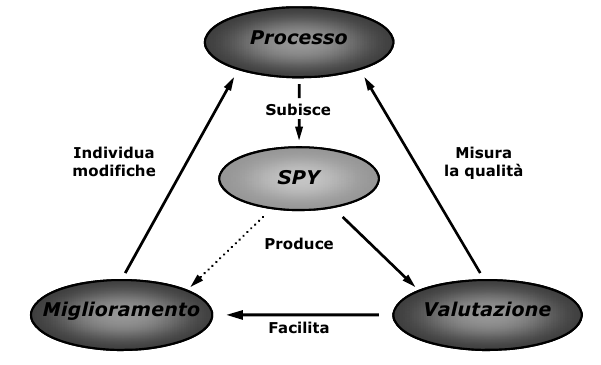
\includegraphics[width=.6\textwidth]{spy}
\caption{Il modello SPY per la valutazione della qualità di processo.}\label{fig:spy}
\end{figure}

La qualità di processo è parte fondamentale del processo per garantire la qualità del prodotto, e viene controllata ponendo come riferimento una serie di attributi specifici:

\begin{description}
\item \inglese{\textbf{Process performance}}: un processo raggiunge gli obiettivi prefissati trasformando input identificabili in output identificabili;

\item \inglese{\textbf{Performance managment}}: un processo è pianificato e controllato allo scopo di produrre risultati coerenti e corrispondenti agli obbiettivi per cui è stato attuato;

\item \inglese{\textbf{Work product management}}: un processo è pianificato e controllato allo scopo di produrre risultati documentabili, controllati e verificabili;

\item \inglese{\textbf{Process definition}}: l'attuazione di un processo si basa su un approccio stardardizzato;

\item \inglese{\textbf{Process resource}}: ogni processo ha a disposizione le adeguate risorse per essere attuato;

\item \inglese{\textbf{Process measurement}}: le misure e i risultati rilevati durante l'attuazione di un processo vengono usati per assicurarsi che lo stesso avvenga per raggiungere efficacemente gli obiettivi prefissati;

\item \inglese{\textbf{Process control}}: ogni processo è controllato mediante la raccolta, l'analisi e l'utilizzo delle misure di processo e di prodotto, al fine di valutare ed eventualmente correggere le sue modalità di attuazione;

\item \inglese{\textbf{Process change}}: il controllo sulle modifiche di gestione, attuazione o definizione di un processo è costante;

\item \inglese{\textbf{Continuous improvement}}: le modifiche e gli accorgimenti su un processo sono identificati e implementati allo scopo di assicurare il continuo miglioramento al fine di raggiungere più efficacemente gli obbiettivi rilevati.
\end{description}

Il modello fornisce inoltre una scala di valutazione sul grado di maturità dei processi, composta da cinque livelli e riportata in figura~\ref{fig:cmmi}. Il livello raggiunto dai fornitori viene utilizzato come ``biglietto da visita'' nella candidatura ai bandi. Questo significa che quanto più elevato è il livello raggiunto dal fornitore tanto migliore è la presentazione che offre di se stesso sullo specifico processo.

\begin{figure}[h]
\centering
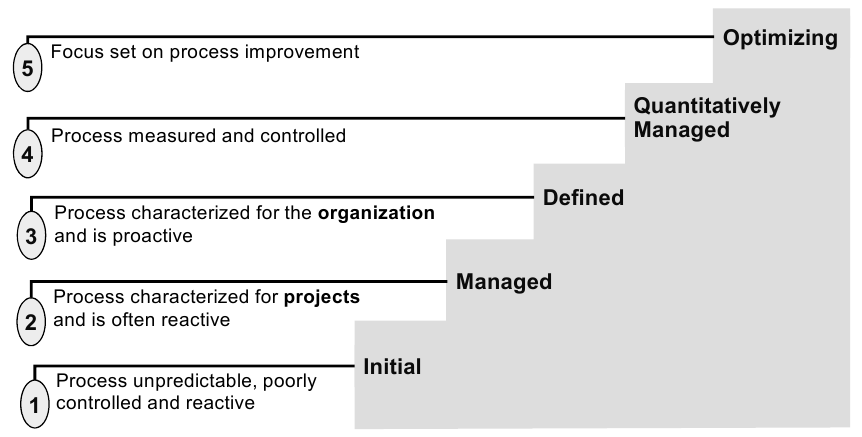
\includegraphics[width=.7\textwidth]{cmmi}
\caption{I livelli della classificazione CMMI.}\label{fig:cmmi}
\end{figure}

\begin{itemize}
\item \textbf{Livello 0}: processo non implementato o incapace di raggiungere gli obiettivi prefissati, non vi è inoltre evidenza di alcun approccio sistematico agli attributi definiti;

\item \textbf{Livello 1}: Il raggiungimento di questo livello è dimostrato attraverso l'attributo specifico \inglese{Process performance} in quanto il processo è messo in atto e raggiunge gli obbiettivi prefissati, tuttavia non è evidente nessun approccio sistematico per nessuno degli attributi definiti;

\item \textbf{Livello 2}: il raggiungimento di questo livello è dimostrato attraverso il possesso degli attributi di \inglese{Performance management} e \inglese{Work product management}. Il processo è gestito e sulla base di obbiettivi definiti è pertanto attuato, pianificato, tracciato, verificato ed eventualmente corretto;

\item \textbf{Livello 3}: il raggiungimento di questo livello è dimostrato attraverso il possesso degli attributi di \inglese{process definition} e \inglese{process resource}. Il processo è definito e sulla base di procedure definite sui principi del \inglese{software engineering} è pertanto attuato, pianificato e controllato;

\item \textbf{Livello 4}: il raggiungimento di questo livello è dimostrato attraverso il possesso degli attributi di \inglese{process measurement} e \inglese{process control}. Il processo risulta ora predicibile, è stabilizzato ed attuato e rispetta i risultati attesi nonché le performance e le risorse impiegate;

\item\textbf{Livello 5}: il raggiungimento di questo livello è dimostrato attraverso il possesso degli attributi di \inglese{process change} e \inglese{continuous improvement}. Il processo si presta all'ottimizzazione, è predicibile e in grado di adattarsi al raggiungimento di obbiettivi specifici e rilevanti a livello organizzativo.
\end{itemize}
\clearpage
%il clearpage serve solo a rendere più leggibile il testo, se modifichiamo il pezzo sopra verrà tolta.

La qualità dei processi, come già accennato ad inizio sezione, è una condizione necessaria per arrivare ad un prodotto di qualità. Il team si pone l'obiettivo di garantire e ottimizzare la qualità dei propri processi mediante l'utilizzo di strumenti necessari per garantirla, pertanto si aspetta di trarre da tali considerazioni:

\begin {itemize}
\item [-] un ottimizzazione dell'uso delle risorse;
\item [-] una migliore gestione economica, contenendo al massimo i costi;
\item [-] una maggiore possibilità di confronto con delle \inglese{best practice};
\item [-] maggiore affidabilità nei tempi di stima rispetto alle consegne preventivate;
\item [-] una migliore stima dei rischi e la loro gestione;
\end {itemize}

Inoltre ogni processo sarà definito in modo dettagliato e valutato l'output prodotto. Infine verranno attuate procedure di misurazione, valutazione ed eventuale modifica sul processo per perseguire il suo miglioramento mediante una costante collaborazione tra il verificatore e lo sviluppatore del processo stesso.

\subsection{Qualità di prodotto software}
Al fine di garantire un elevato standard qualitativo, sia per ovvia scelta del team di sviluppo, sia per implicita richiesta da parte del committente stesso, \team{} ha preso come riferimento lo standard ISO/9126:2001.

\begin{description}
\item{\bfseries Funzionalità}
Il prodotto \caName{} deve soddisfare nelle sue funzionalità tutti i requisiti obbligatori individuati nell'attività di analisi, garantendone il funzionamento e l'aderenza alle richieste specifiche del committente. Tutto questo sarà svolto nel modo meno oneroso sia dal punto di vista economico che di sfruttamento delle risorse disponibili.

Per valutare il grado di funzionalità raggiunto dal prodotto si valuterà la quantità di requisiti che sono stati correttamente implementati all'interno del software finale. La soglia minima di soddisfacimento risulta essere l'assoluta copertura dei requisiti obbligatori imposti dal committente, tuttavia è parso chiaro che la fantasia del team in questa specifica area sarà ben valutata.

\item{\bfseries Portabilità}
Il prodotto finale dovrà per vincoli di capitolato essere pianamente usufruibile mediante browser \underline{Chrome}, prodotto da Google, su tutti i sistemi operativi sui quali questo browser risulta compatibile.

A dimostrazione di tale soddisfacimento ci si affida alla dimostrazione del superamento della validazione del codice del \inglese{front-end web} e dell'assoluta coerenza con le specifiche \underline{WebRTC}, proposta evolutiva di \underline{HTML5}.
All'approvazione del superamento di tale requisito si procederà con lo stesso metodo testando browser alternativi a quello imposto al fine di rendere \caName{} usufruibile da un bacino d'utenza più vasto possibile.

\item{\bfseries Usabilità}
Il prodotto deve risultare facile ed intuitivo da parte dell'utenza che dispone di una conoscenza medio-bassa del web e dell'informatica in generale.

Utenti che hanno familiarità con programmi per la gestione di chiamate mediante \underline{VOIP} non dovranno trovare alcuna difficoltà o iniziale disorientamento nell'utilizzo di \caName{}.

Data l'aleatorietà di tale qualità di prodotto e la non ``oggettività'' nella misurazione di tale caratteristica si cercherà semplicemente di raggiungere tale risultato basandosi su esperienze personali o brevi test su specifici utenti selezionati.

\item{\bfseries Affidabilità}
L'applicazione deve riuscire a stabilire e mantenere stabile una comunicazione tra due o più utenti, senza mostrare problemi di natura tecnica se non imputabili alla qualità della connessione di cui dispongono gli utenti stessi. Deve dimostrarsi altresì robusta nella sua struttura e facile da ripristinare in caso di errori di varia natura.

Al fine di garantire queste caratteristiche verrà utilizzata come unità di misura la quantità di interazioni tra utenti con esito positivo, tenendo conto di tutti i parametri che concorrono ad una corretta comunicazione (qualità audio, video, messaggi testuali correttamente inviati/ricevuti, etc.).

\item{\bfseries Efficienza}
\caName{} si pone come obbiettivo oltre alla corretta ed appagante esperienza comunicativa, anche di non risultare particolarmente esosa dal punto di vista hardware, sia dal punto di vista puramente componentistico dell'unità dalla quale si accede al prodotto, sia dal punto di vista dell'uso di banda a disposizione della rete.

Verranno pertanto monitorate in fase di test sia le percentuali d'utilizzo di memoria e processore della macchina, sia la quantità di kb/s trasmessi e ricevuti durante l'esecuzione del programma. I test verranno eseguiti su varie tipologie di hardware e linee di diverse velocità, al fine di rendere il software usufruibile dalla più vasta fetta d'utenza possibile.

I test risulteranno superati se nei momenti di massimo consumo di risorse il programma riuscirà a garantire un utilizzo fluido e una discreta navigabilità nel web dalla macchina soggetta al test. 

\item{\bfseries Manutenibilità}
Il capitolato specifica esplicitamente che la modifica e la manutenibilità del software sono una caratteristica fondamentale dell'intero progetto, questa necessità nasce dal costante utilizzo di linguaggi non ancora qualificati come standard, pertanto soggetti a continua evoluzione.
\end{description}

\subsubsection{Ciclo di Deming}
Per riscontrare e raggiungere le caratteristiche sopra elencate il team ha deciso di adottare il \underline{ciclo di Deming} (PDCA)\@.

\begin{figure}[h]
\centering
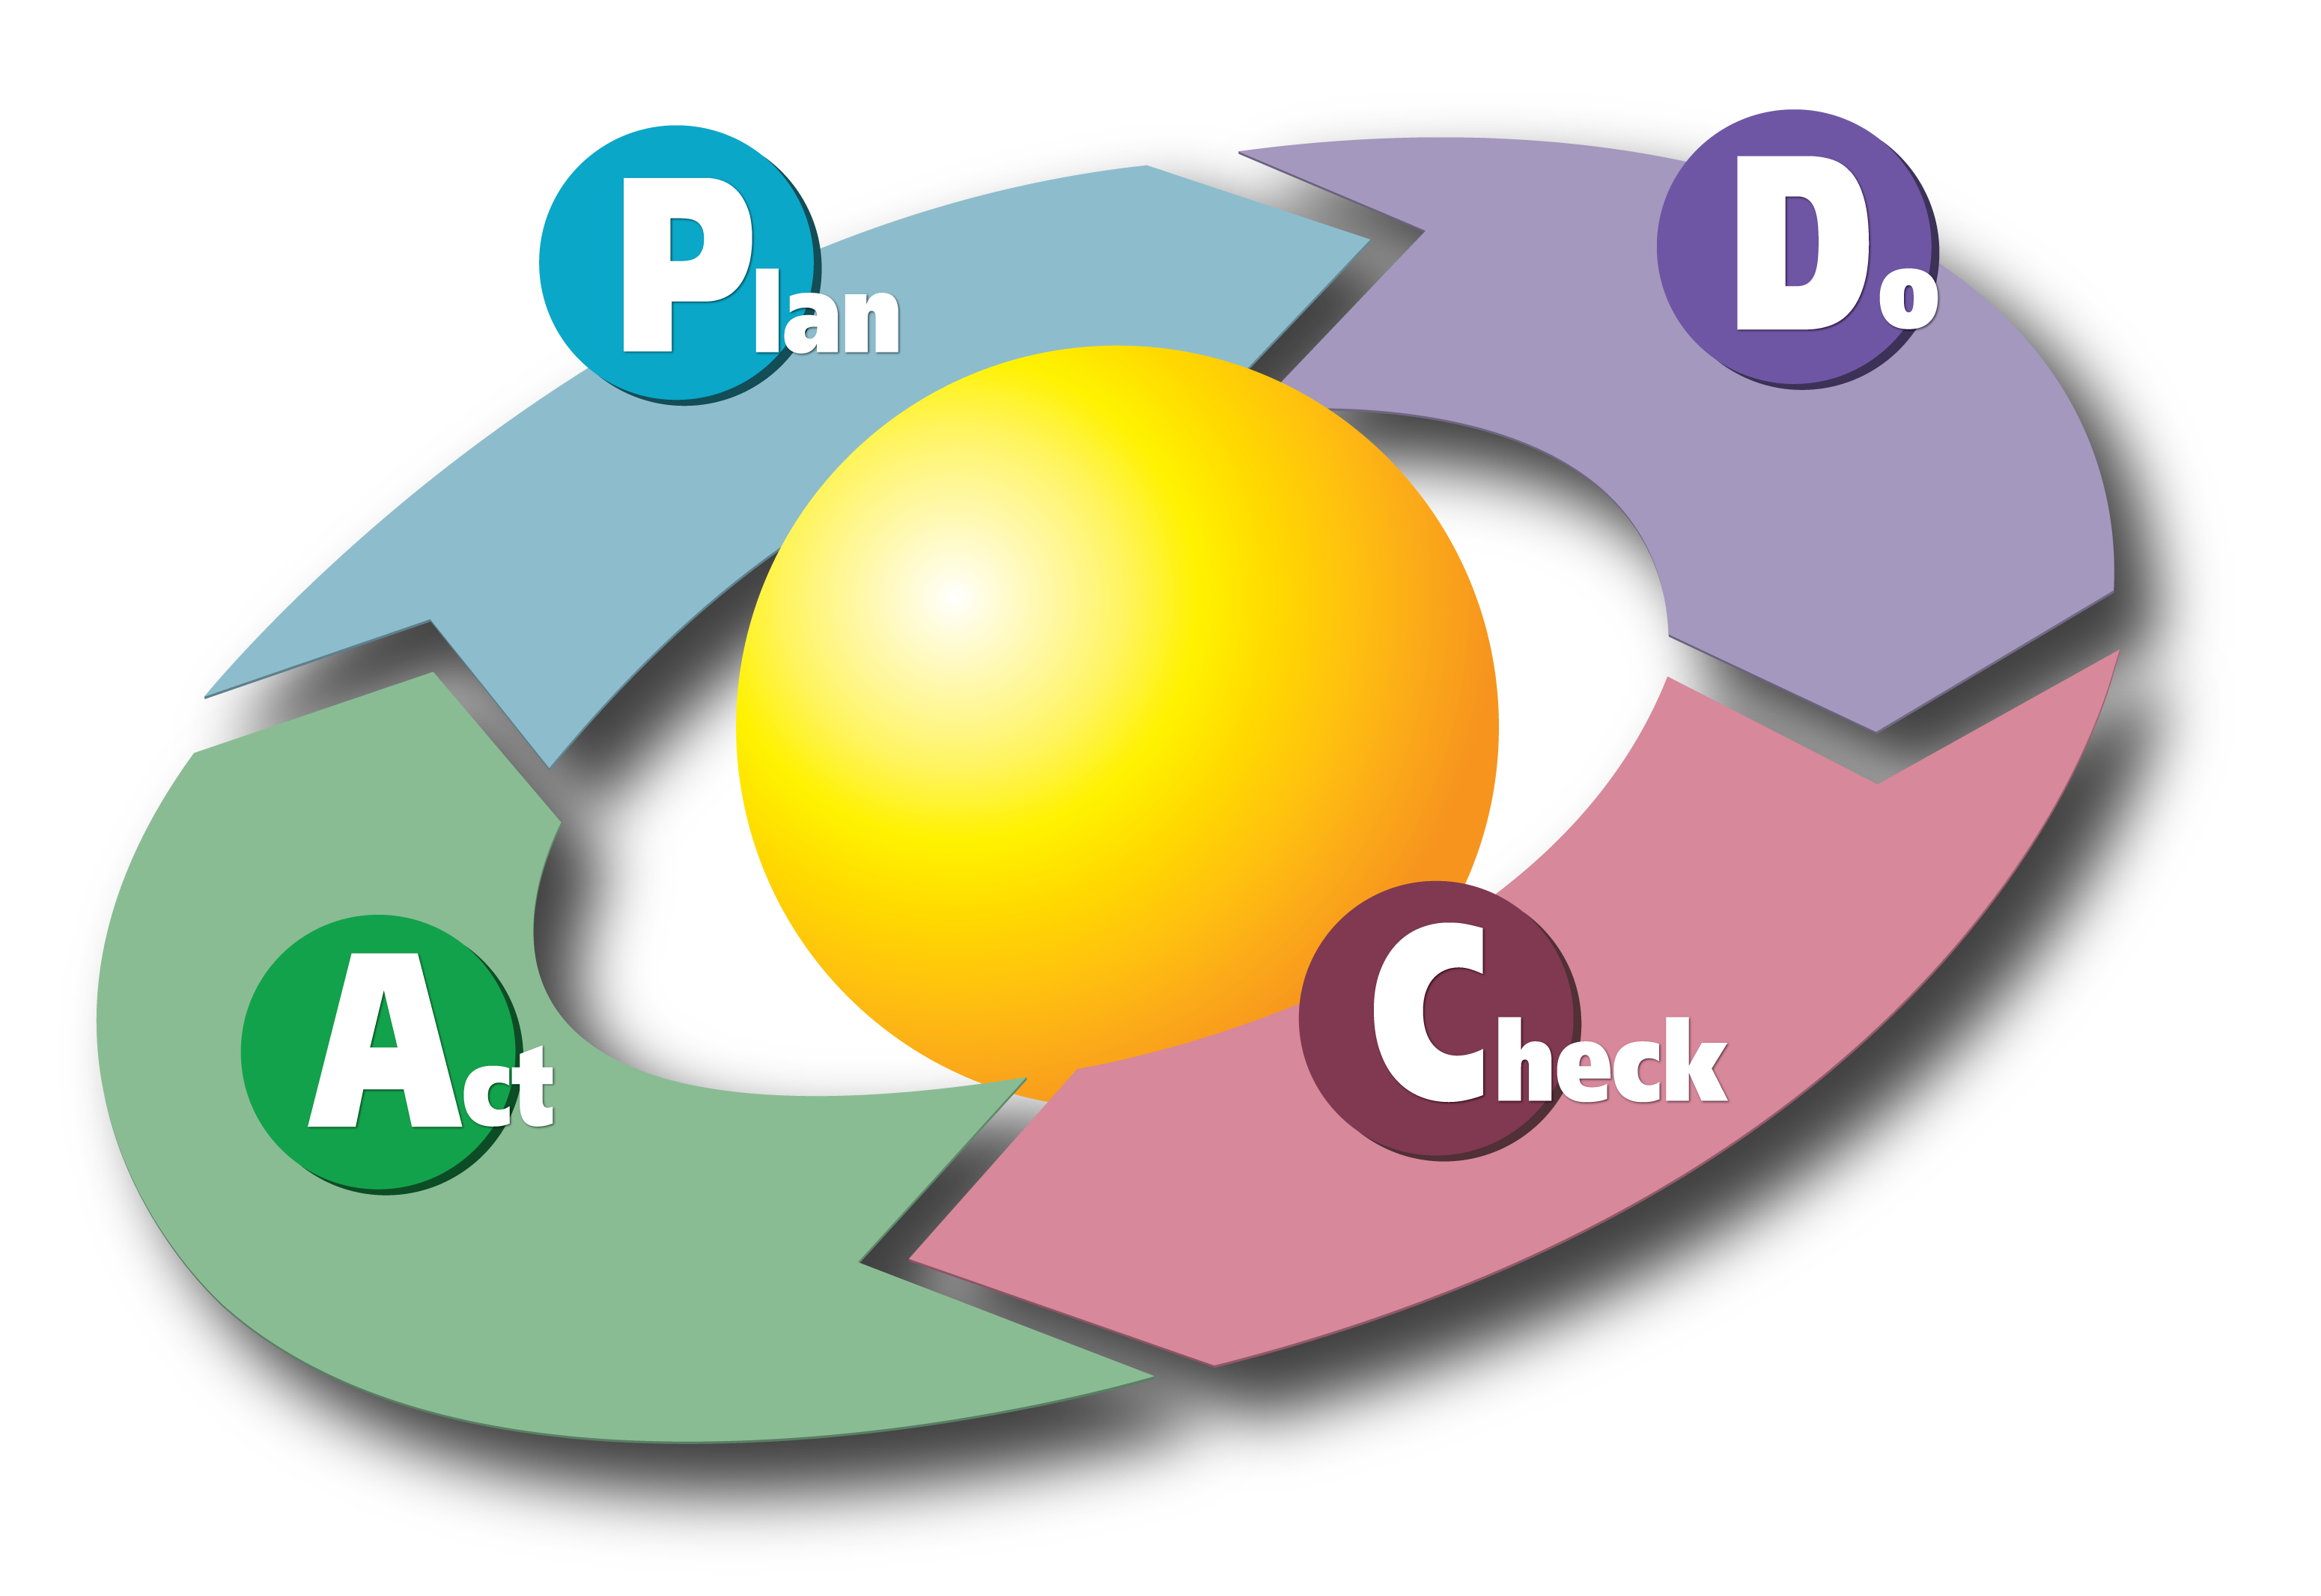
\includegraphics[width=.35\textwidth]{pdca}
\caption{Il ciclo di Deming.}\label{fig:pdca}
\end{figure}

Tale tecnica è costituita dalle seguenti fasi:

\begin{tabularx}{.9\textwidth}{>{\bfseries\scshape}lX}
plan  & analizzare il problema e stabilire le attività, le tempistiche e i soggetti coinvolti;\\
do    & attuare dettagliatamente le attività pianificate;\\
check & verificare a consuntivo quanto preventivato nella pianificazione;\\
act   & nel caso in cui il controllo abbia rilevato discrepanze tra preventivo e consuntivo attuare misure correttive.\\
\end{tabularx}

Gli obiettivi di qualità prefissati possono essere raggiunti tramite una adeguata pianificazione delle attività, che deve essere rispettata attentamente per poter permettere l'autovalutazione ed eventualmente l'adozione di misure correttive volte al miglioramento continuo e all'attuazione delle \underline{\inglese{best practices}}.  Solo in tal modo è infatti possibile ottenere un prodotto di qualità.

\subsection{Gestione della qualità}
La qualità di un software non si limita all'assenza di problematiche durante il suo funzionamento  anche se è evidente che la maggior parte delle attività inerenti al suo controllo hanno come fine ultimo l'identificazione e l'eliminazione di ogni possibile caratteristica che si discosti dal comportamento atteso del programma o dai requisiti che il programma stesso deve soddisfare.

Al fine di rendere ancor più chiara la comprensione di tali problematiche ed evitare che termini all'apparenza simili assumano significati impropri precisiamo che un \underline{\textbf{malfunzionamento}} è un funzionamento di un programma (o di una sua parte) diverso da quanto previsto dalla sua specifica, un \underline{\textbf{difetto}} è la causa di un malfunzionamento, mentre un \textbf{errore} è l'origine di un difetto.
Tali termini oltre ad avere un significato diverso hanno quindi anche una dipendenza causa-effetto gli uni dagli altri, con una dipendenza temporale ben definita.

Terminiamo il capitolo evidenziando gli aspetti fondamentali per contenere i problemi descritti in precedenza e accertare la qualità del prodotto e dei processi: \inglese{Quality Assurance}, Verifica e validazione.
Nel primo caso si intende l'insieme della attività svolte a garantire il soddisfacimento degli obbiettivi di qualità prefissati, mentre la verifica deve garantire che avvengano i controlli affinché il prodotto ottenuto al termine di una fase sia coerente con quanto precedente a tale fase. La Validazione è infine un'attività di controllo che confronta il risultato di una fase del processo di sviluppo del prodotto con i requisiti del prodotto stesso.\\

Verifica e validazione sono attività che coesistono con quelle tradizionali, e la loro integrazione deve essere svolta nel modo più efficace possibile al fine di renderle concretamente produttive in quanto la scoperta di un errore durante lo sviluppo garantisce un guadagno significativo per la qualità del prodotto.
\clearpage

\section{Visione generale della strategia di verifica}

\subsection{Organizzazione, pianificazione strategica, pianificazione temporale e responsabilità}
L'attività di verifica inizierà quando il prodotto di un processo raggiungerà uno stadio che si potrà definire diverso da quello precedente a seguito della conclusione di un processo di ciclo di vita.

La verifica di tali cambiamenti sarà operata in modo mirato e circoscritta, grazie al registro delle modifiche che verrà compilato durante la stesura del documento stesso. Al termine della fase di verifica, i documenti saranno consegnati al responsabile di progetto, che provvederà ad approvarli.

Il team nel \underline{\inglese{brainstorming}} successivo all'analisi generale del progetto \caName{} ha deciso di adottare un ciclo di vita incrementale (specificato nel documento \textit{piano\_di\_progetto.3.0.pdf}).

Coerentemente a tale scelta, il processo di verifica adottato opererà nelle diverse fasi del progetto nel modo seguente:

\subsubsection{Analisi dei Requisiti}
Quando un documento uscirà dalla fase di redazione, verrà preso in esame ed effettuata una fase di revisione definitiva prima di essere presentato ufficialmente alla RR: 
\begin{itemize}
  \item[-] Verrà presa in esame la correttezza grammaticale, che al contrario di quella ortografica può essere verificata solo mediante un accurata rilettura da parte del verificatore designato.
  \item[-] Verrà presa in esame la correttezza lessicale mediante un'accurata rilettura da parte del verificatore designato.
  \item[-] Verrà presa in esame la correttezza dei contenuti e la coerenza rispetto al documento mediante un accurata rilettura da parte del verificatore designato.
  \item[-] Verrà effettuata la verifica che ogni tabella o figura sia corretta nel suo contenuto e disponga della rispettiva didascalia.
  \item[-] Verrà presa in esame la correttezza rispetto alle norme di progetto redatte, utilizzando gli strumenti più appropriati per la verifica.
  \item[-] Verrà presa in esame la corrispondenza tra ogni requisito e i casi d'uso, consultando e controllando le apposite tabelle di tracciamento, verificando inoltre la corretta gestione di entrambi mediante \manager, l'applicativo web creato appositamente da \team.
  \item[-] Verrà considerata la corrispondenza fra i requisiti elencati e quanto enunciato nel testo del capitolato, in modo da assicurare che tutti i requisiti espliciti siano stati correttamente recepiti.
  \item[-] Verrà presa in esame la chiarezza espositiva nell'enunciazione dei requisiti al fine di ridurre al minimo le ambiguità nonché la granularità dei requisiti individuati, perché avere requisiti atomici ne rende più facile il tracciamento e la verifica del soddisfacimento.
\end{itemize}

\subsubsection{Progettazione}

\subsubsection*{Progettazione ad alto livello}
Il processo di verifica garantirà la rintracciabilità nei componenti individuati durante la fase di Progettazione architetturale di ogni singolo requisito descritto nel documento di analisi dei requisiti (versione 4.0). A tale scopo lo strumento che si è scelto di utilizzare è ancora \manager, nello specifico tramite il modulo relativo ai \inglese{configuration item}.

Tali verifiche verranno svolte al termine della stesura del documento di specifica tecnica e dell'aggiornamento dei documenti relativi al piano di progetto, piano di qualifica, norme di progetto, analisi dei requisiti.

Al fine di garantire un'elevata qualità nell'architettura software elaborata durante la progettazione di alto livello, la verifica dovrà valutare la presenza delle seguenti proprietà:
\begin{itemize}
\item \textbf{necessità} ogni componente soddisfa almeno uno fra i requisiti emersi in fase di analisi;
\item \textbf{sufficienza} l'architettura nel suo complesso è in grado di soddisfare tutti i requisiti;
\item \textbf{modularità} è chiaramente definita la suddivisione delle varie componenti e il ruolo di ciascuna di esse;
\item \textbf{flessibilità} permette modifiche a basso costo al variare dei requisiti;
\item \textbf{affidabilità} consente un utilizzo corretto durante il funzionamento;
\item \textbf{semplicità} ogni parte contiene tutto e solo ciò che è necessario al proprio funzionamento;
\item \textbf{incapsulamento} le parti del sistema mantengono private le informazioni relative al proprio stato interno e permettono di accedervi solo attraverso le operazioni dell'interfaccia pubblica che espongono verso l'esterno;
\item \textbf{coesione} le componenti che stanno assieme condividono lo stesso obiettivo;
\item \textbf{basso accoppiamento} eventuali modifiche a una componente avranno bassa o nulla incidenza sul resto dell'architettura grazie al controllo delle relazioni di dipendenza.
\end{itemize}

Infine, i diagrammi UML riportati nel documento di specifica tecnica saranno sottoposti a verifica rispetto a quanto stabilito nella sezione 3.4 del documento \textit{norme\_di\_progetto.3.0.pdf}.

\subsubsection*{Progettazione di dettaglio}
Per ogni unità architetturale prodotta durante la fase di progettazione di dettaglio verrà effettuato un test di unità al fine di verificarne il comportamento dell'unità stessa rispetto a quello atteso in fase d'esecuzione. Tali test sono definiti da:
\begin{itemize}
  \item un oggetto su cui viene eseguito e gli obbiettivi del il test;
  \item la strategia e le risorse software utilizzate nella prova;
  \item il piano d'esecuzione del test stesso.
\end{itemize}

Allo scopo di ridurre al minimo la presenza di errori interni alle singole unità sono stati programmati un numero di test sufficiente ad assicurare \inglese{statement coverage} e \inglese{branch coverage}, la prima ha lo scopo di assicurare che tutte le linee di comando di ciascun modulo siano state eseguite almeno una volta, mentre la seconda assicura che tutti i possibili rami del flusso di controllo vengono attraversati almeno una volta.

Effettuati i test di unità si procederà con l'unione delle unità stesse in modo da poter effettuare i relativi test d'integrazione per verificare come le varie componenti del sistema interagiscono tra loro, evidenziando eventuali difetti di progettazione, e dipendenze (o incompatibilità) tra i diversi componenti architetturali.

La pianificazione dei vari test da eseguire verrà fornita dal team \team{} una volta terminata la fase di progettazione di dettaglio.

\subsubsection{Codifica}
I programmatori svolgeranno le attività di codifica del prodotto e i test di unità per la verifica del codice realizzato nel modo più automatizzato possibile.

I verificatori inoltre controlleranno la presenza di eventuali discrepanze rispetto alle norme pattuite in merito al processo di codifica, nonché l'identificazione di parti di codice soggette ad errori di programmazione.
I modelli presi in considerazione per eseguire tali verifiche sono due: verifica funzionale e verifica  strutturale.

La verifica funzionale (\underline{\inglese{black-box}}) è una tecnica che procederà con l'accertamento delle funzionalità di un unità controllando esclusivamente che i risultati in uscita rispecchino il valore atteso in ogni condizione d'utilizzo che l'unità dispone. Questo tipo di modello consente test efficaci sull'intero sistema o su unità di dimensioni rilevanti.

La verifica strutturale (\underline{\inglese{white-box}}) al contrario è una tecnica in cui l'ispezione viene svolta a livello di codice sorgente, richiamando esplicitamente tutti i metodi presenti nell'unità al fine di verificarne, oltre al corretto funzionamento, anche la correttezza logica. Questo modello si predilige per controlli sui singoli moduli che costituiscono il progetto, controllando come già citato la struttura stessa del codice.

Specifichiamo infine che per effettuare un controllo approfondito del codice si utilizza il termine ``analisi'', che si specializza essenzialmente in due tipologie: analisi statica e dinamica.

L'analisi statica non comporta l'esecuzione del codice in quanto la verifica avviene tramite lettura da parte di un verificatore (tramite \underline{\inglese{inspection}} e \underline{\inglese{walkthrough}}, descritti più dettagliatamente nella sezione 5.1.1) o mediante opportuni strumenti software di verifica statica. Gli errori riscontrati mediante tali metodologie dal verificatore non vengono corretti dal soggetto stesso, ma vengono riferiti al progettista o al programmatore al quale comunque rimane il compito di individuazione e correzione degli errori individuati durante il suo lavoro sul codice stesso.
L'analisi dinamica richiede l'esecuzione del programma in un ambiente controllato e con dati in ingresso verificati. Verranno registrati tutti i dati relativi all'esecuzione e inerenti alla quantificazione della qualità del software preso in esame, inoltre tali dati saranno confrontati con i requisiti stilati.

    
\subsubsection{Validazione}
Alla fase di collaudo, il team garantirà il corretto funzionamento del prodotto \caName{} relativo alle funzionalità,l'usabilità, l'efficienza, l'affidabilità, e la portabilità. Tali garanzie vengono confermate dopo un'attività interna di test denominata Alfa-test. All'esito positivo di tale attività avverrà il collaudo vero e proprio (Beta-test) alla presenza del proponente, successivi \underline{difetti} riscontrati o eventuali caratteristiche non coerenti alle richieste di quest'ultimo saranno soggette a modifica e correzione al fine di eliminare tali incongruenze.
\clearpage

\subsection{Risorse necessarie e disponibili}
L'utilizzo di risorse umane e tecnologiche è fondamentale per la verifica di qualità del prodotto e dei processi.

\subsubsection{Umane}
\team{} si è imposta, per garantire un elevato standard qualitativo, che all'interno del team siano ricoperti, nel corso del progetto, i seguenti ruoli:

\begin{itemize}
\item Responsabile: responsabile della corretta realizzazione del prodotto secondo gli standard e le richieste commissionate, designato all'allocazione corretta delle risorse umane ai rispettivi compiti e stimolarne il coordinamento. 
Controlla inoltre la qualità dei processi interni mediante le attività di verifica da lui predisposte. Infine ha la facoltà di approvare o meno ogni proposta di correzione (migliorativa o di modifica generica) avanzata.
\item Amministratore: stila le metodologie e definisce le norme per la verifica dei processi, gestisce inoltre i risultati relativi ai test eseguiti e il processo di gestione e correzione delle anomalie e delle discrepanze.
\item Verificatore: applica i processi di verifica e validazione approvati dall'amministratore e predisposte dal responsabile tenendo traccia del suo lavoro. Ogni discrepanza o anomalia incontrerà durante tale attività verrà presentata tramite \inglese{ticketing} (vedi capitolo 5 del documento \textit{norme\_di\_progetto.3.0.pdf}).
\item Programmatore: durante il suo lavoro ha l'obbligo di risolvere le anomalie evidenziate tramite \inglese{ticketing} dai verificatori o dai test effettuati sul codice da lui stesso prodotto.
\end{itemize}

\subsubsection{Software}
A livello software risulteranno necessarie, le seguenti risorse:

\begin{description}
\item{\bfseries \manager}, il programma basato su interfaccia web sviluppato internamente al team per il tracciamento e la gestione dei requisiti avente lo scopo di standardizzare e rendere quanto più automatizzata possibile tale fase del progetto ed evitare quindi l'insorgere di eventuali sviste dovute all'intervento umano.

\item{\bfseries Sistema di controllo versione} (in particolare \texttt{git}) al fine di permettere il lavoro in parallelo da parte dei membri del gruppo e la gestione dello storico delle versioni; il gruppo prevede altresì di appoggiarsi a un \underline{\inglese{repository}} remoto per permettere la sincronizzazione fra i diversi utenti (cfr.~sez.~3.1 del documento \textit{norme\_di\_progetto.3.0.pdf}). 

\item{\bfseries Editor di diagrammi}, da impiegarsi tanto per la produzione dei diagrammi UML richiesti per l'attività di progettazione quanto per la creazione dei diagrammi di Gantt necessari alla pianificazione delle attività di progetto. 

\item{\bfseries \underline{Sistema di \inglese{ticketing}}}, per gestire la suddivisione e l'assegnazione delle attività ai vari componenti del gruppo in maniera ordinata e controllabile.

\item{\bfseries Ambiente di sviluppo integrato (\underline{IDE})}, al fine di individuare e correggere già durante l'attività di codifica gli eventuali errori presenti nel codice nonché di renderne più agevole la ristrutturazione (\inglese{refactoring}).

\item{\bfseries Analizzatori statici}, vale a dire strumenti per permettere l'automatizzazione nell'analisi del codice prodotto, ai fini di ricavarne il maggior numero possibile di informazioni. Le risorse da utilizzare a tale scopo sono descritte con maggiori dettagli nella sezione~8.1 delle norme di progetto (versione 2.0).

\item{\bfseries \inglese{Testing framework}}, che risulteranno utili ai fini dei test di unità legati al linguaggio di programmazione scelto per standardizzare (e automatizzare) i test sul prodotto finale nonché produrre dei resoconti appropriati sulle eventuali anomalie riscontrate.

\item{\bfseries \inglese{Editor} di documenti}, secondo quanto documentato nella sezione~4.1 delle norme di progetto (versione 2.0), in particolare un editor di testo specializzato per \LaTeX con evidenziazione della sintassi, auto-completamento dei comandi e correzione ortografica integrata. 
\end{description}

Gli specifici programmi e \inglese{tool} per la gestione di tali servizi sono descritti in dettaglio nel documento \textit{norme\_di\_progetto.3.0.pdf} allegato.

\subsubsection{Hardware}
\team{} ha a disposizione oltre al materiale personale di ogni componente del team (computer portatili e fissi) le strutture fisiche ed informatiche messe a disposizione dalla facoltà di informatica dell'Università degli Studi di Padova, quali laboratori didattici e le aule studio allocate negli stabili della Facoltà stessa.
\clearpage


\section{Tecniche, metodi e metriche}

\subsection{Tecniche}
Durante lo svolgimento del progetto il team utilizzerà le tecniche di analisi statica e dinamica per effettuare verifiche su software e documentazione.

\subsubsection{Analisi statica} 
L'analisi statica è un tipo di controllo basato sulla non esecuzione del codice, ma in senso lato può essere applicato a qualsiasi tipo di prodotto anche non propriamente eseguibile (ad es. la documentazione di progetto). Sono previste, in particolare, due forme di analisi statica: il controllo manuale (detto altrimenti \inglese{desk check}) e il controllo assistito da strumenti automatici.
Per quanto concerne il \inglese{desk check}, cioè il controllo realizzato unicamente da parte di un agente umano, sono previsti due metodi formali:

\begin{itemize}
\item \textbf{\underline{walkthrough}}: implica un esame ad ampio spettro del prodotto da verificare, che è preso in considerazione nella sua totalità in modo indiscriminato e senza alcuna assunzione previa sulla natura, la posizione e la frequenza degli errori da rilevare. Si tratta notoriamente di una tecnica molto onerosa in termini sia di tempo che di sforzo e può essere essa stessa per sua natura soggetta ad errori (in particolar modo falsi negativi). Tuttavia, almeno nelle fasi iniziali del lavoro, è l'unica scelta praticabile a causa della relativa inesperienza dei membri del gruppo nella realizzazione di prodotti complessi e articolati (sia software che documentazione). Allo scopo di ridurre il costo determinato dalla ripetizione di tale attività nell'arco di tutto il ciclo di vita è previsto che durante l'analisi in \inglese{walkthrough} sia stilata una lista di controllo relativa agli errori più frequenti e ai contesti in cui è più probabile che si producano errori in modo da collezionare una base di esperienza comune e consolidata destinata ad alimentare le attività di ispezione.

\item \textbf{\underline{inspection}}: prevede un controllo mirato avente obiettivi specifici, ristretti e stabiliti a priori \textit{prima} che la verifica abbia luogo. Si tratta di un'attività meno dispendiosa in termini di risorse perché non presuppone l'analisi esaustiva del prodotto ma è focalizzata su determinate categorie di errori frequenti, enunciate in una lista di controllo (\inglese{checklist}) redatta sulla base dell'esperienza personale e delle attività di \inglese{walkthrough} precedentemente poste in essere.
\end{itemize}


\subsubsection{Analisi dinamica} 
I controlli dinamici, altrimenti definiti test, prevedono l'esecuzione del software in un ambiente controllato e con dati di input specificatamente pensati per testarne le funzionalità e l'aderenza ai requisiti mettendo in luce l'eventuale presenza di malfunzionamenti dovuti alla presenza di difetti.

Caratteristica fondamentale dei test è la loro \textbf{ripetibilità}, cioè dato lo stesso set di dati in ingresso e nello stesso contesto di esecuzione, l'output deve essere deterministico e univocamente determinato. Tale proprietà, unitamente all'auspicabile utilizzo di un \inglese{logger} che ha il compito di registrare le fasi dell'esecuzione del test, consente di individuare e riconoscere in maniera più agevole i difetti presenti nel prodotto.

In base al loro ambito di applicazione, i test possono essere suddivisi in:
\begin {itemize}
\item test di unità aventi come oggetto le singole unità e, oltre al modulo da verificare e ai dati d'esempio, possono coinvolgere anche componenti attive (\underline{driver}) o passive (\underline{stub}) che siano in grado di simulare le parti del sistema non ancora disponibili al momento in cui il test viene eseguito;

\item test di integrazione atti a verificare la corretta interazione e integrazione fra le componenti che costituiscono le parti del sistema e hanno come risultato una \inglese{build}, vale a dire un sottosistema funzionante che può essere eseguito in modo indipendente;

\item test di sistema, volti a testare il rispetto dei requisiti software individuati in fase di analisi dei requisiti da parte dell'intero sistema;

\item test di regressione destinati a rilevare il caso indesiderabile in cui una modifica locale destabilizza il resto del sistema, si tratta del numero minimo di test necessario per scongiurare tale eventualità senza per questo dover ripetere in toto i test di unità e di integrazione;

\item test di accettazione, o collaudo, realizzato sotto la supervisione del committente per verificare l'aderenza del prodotto ai requisiti utente di più alto livello.

\end{itemize}

\subsection{Metodi}
Il processo di misurazione attraverso il quale è possibile valutare quantitativamente l'aderenza del prodotto agli standard di qualità è basato su un ciclo iterativo simile al ciclo di Deming. In particolare, in una fase preliminare prevede che sia stabilita l'importanza e l'ambito di applicazione della misurazione, la selezione di metriche da adottare come si è fatto nelle precedenti sezioni e la pianificazione del momento nel ciclo di sviluppo in cui le misurazioni dovranno essere effettuate.

La parte operativa, cioè la quantificazione dei valori delle metriche di qualità, avviene lungo tutto l'arco del ciclo di sviluppo, con particolare attenzione alle fasi di progettazione di dettaglio e di test effettuati contestualmente alla codifica e in fase di accettazione/collaudo.

Al fine di evitare che la verifica della qualità sia un onere troppo gravoso in termini di risorse umane e di tempo, anch'esso deve essere sottoposto a misurazione in quanto attività di progetto (cioè la parte \inglese{check} di PDCA): il tempo di lavorazione impiegato per attività di verifica e \underline{QA} dovrà dunque essere registrato in ogni momento, ed è prerogativa del responsabile di progetto adottare misure correttive qualora i tempi dovessero risultare eccessivi al punto da compromettere il rispetto delle scadenze stabilite nel piano di progetto.

Il team ha quindi, dopo aver analizzato il problema che andrà ad affrontare, optato per utilizzare le seguenti tipologie di analisi statica: 
\begin{itemize}

\item \textbf{Analisi di flusso di controllo:} il prodotto sviluppato avrà caratteristiche di affidabilità e robustezza, riducendo al minimo gli sprechi. Questa analisi ha il compito di verificare che il codice sia eseguito nella giusta sequenza, correttamente strutturato, e non siano presenti parti di codice non raggiungibili o iterazioni aventi un limite superiore non definito. A tale fine sarà necessario prestare particolare attenzione alle decisioni interne all'unità di codice e verificare che le condizioni risultino totalmente gestite.

\item \textbf{Analisi di flusso dei dati:} al fine di garantire che in ogni stato in cui si trova il prodotto si riesca ad accedere correttamente ai dati richiesti dall'utente e che nessun cammino d'esecuzione acceda a variabili prive di valore. 
Questa tipologia di analisi può rilevare anomalie quali scritture successive su una variabile senza letture intermedie o la presenza di variabili \inglese{write-only}. Al fine di evitare complicazioni inutili, per questo tipo di analisi si opterà per sconsigliare l'uso di variabili globali in fase di progettazione e codifica.

\item \textbf{Analisi di flusso di informazione:} per controllare il grado di accoppiamento, determinando le dipendenze tra ingressi e uscite che risultano dall'esecuzione di un'unità di codice e consentendo solo quelle previste dalla specifica degli specifici moduli.

\item \textbf{Verifica formale del codice:} garantisce la correttezza del codice sorgente sviluppato rispetto alla specifica formale dei requisiti redatta nell'attività di analisi.
\end{itemize}

\subsection{Metriche}
Per effettuare delle misure efficacemente è necessario definire un'unità di misura, una scala metrica e il metodo per rilevare tali misure.

Tali caratteristiche sono definite dettagliatamente dallo standard ISO/IEC 9126, e le metriche descritte possono essere catalogate secondo due macro categorie: metriche elementari e derivate. Le prime sono in grado di rappresentare istantaneamente un dato fenomeno, le metriche derivate al contrario sono ricavate da operazioni su altre misurazioni.

Sempre in riferimento alla capacità di immediatezza di misurazione sulle caratteristiche del prodotto si possono distinguere metriche dirette, che sono rilevabili sul software senza considerare l'influenza di fattori esterni (come l'ambiente nel quale è eseguito il software), e metriche indirette che combinano nelle misurazioni sul prodotto anche misure relative a elementi ambientali.

\subsubsection{Metriche per il progetto}
Relativamente all'andamento e alla gestione del progetto il team ha stabilito di affidarsi a una serie di indicatori al fine di ottenere una stima delle caratteristiche che per loro natura non possono essere misurate in maniera esatta. L'uso di tali indicatori è stato ritenuto opportuno al fine di valutare l'insorgenza di fattori di criticità e controllare il rispetto dei vincoli in termini di risorse (tempi/costi) di progetto.

Gli indicatori selezionati come candidati per l'utilizzo sono, in particolare:
\begin{description}
  \item{\scshape\bfseries BCWS} (\inglese{Budgeted Cost of Work Scheduled}) pari al costo preventivato in termini di ore per realizzare i \inglese{task} di progetto fino alla data corrente;
  \item{\scshape\bfseries ACWP} (\inglese{Actual Cost of Work Performed}) dato dal costo a consuntivo in termini di ore effettivamente impiegato per lo svolgimento dei \inglese{task} di progetto alla data corrente;
  \item{\scshape\bfseries BCWP} (\inglese{Budgeted Cost of Work Performed}) determinato dal valore delle attività terminate alla data corrente;
  \item{\scshape\bfseries BV} (\inglese{Budget Variance}) definito come \[BV \stackrel{\Delta}{=} BCWS - ACWP \] ovvero lo scostamento fra quanto preventivato e quanto sostenuto in termini di costi alla data corrente;
  \item{\scshape\bfseries CV} (\inglese{Cost Variance}) definito come \[BV \stackrel{\Delta}{=} BCWP - ACWP \] dato dallo scostamento fra il valore di quanto effettivamente prodotto dalle attività di progetto e il costo sostenuto.
\end{description}

\subsubsection{Metriche per la verifica del codice}\label{sec:metrics}

Si riporta un elenco delle principali metriche, in riferimento alle quali il team di sviluppo si ripropone di valutare in modo univoco e quantificabile la qualità del prodotto relativamente alla parte di codifica:

\begin{itemize}
  \item numero di righe di codice esclusi commenti e annotazioni, considerato nella sua totalità (TLOC, \inglese{Total lines of code}) o piuttosto come corpo dei soli metodi (MLOC, \inglese{Method lines of code});
  \item numero di metodi (NOM, \inglese{Number of Methods}) e numero di campi dati di ciascuna classe (NOF, \inglese{Number of Fields});
  \item profondità di una classe nell'albero di derivazione (DIT, \inglese{Depth of Inheritance Tree});
  \item numero di metodi ridefiniti (NORM, \inglese{Number of OverRidden Methods})
  \item indice di specializzazione (IS), definito come \[
  IS \stackrel{\Delta}{=} \frac{DIT \times NORM}{NOM}
  \]
  \item complessità ciclomatica, basata sul concetto che un metodo può essere rappresentato come un grafo, per calcolare tale complessità vengono sommati tutti i cammini linearmente indipendenti di tale metodo: maggiore è il numero di cammini, maggiore sarà di conseguenza la complessità ciclomatica e la possibilità che in tale codice ci siano errori; tale metrica è definita come
  \[v(G)=E-N+P\]
dove $E$ è il numero di archi, $N$ il numero di nodi e $P$ le componenti connesse da ogni arco e risulta essere molto utile per determinare il numero di test da effettuare su un determinato metodo per coprire tutti i cammini possibili;

  \item peso della classe (WMC, \inglese{Weighted Methods per Class}) definito come la somma della complessità ciclomatica di tutti i metodi membri di una classe;
  \item mancanza di coesione dei metodi di una classe (LCOM, \inglese{Lack of Cohesion of Methods}), un indice che misura quanto i metodi di una classe fanno riferimento ai campi dati della stessa, definito se $m(A)$ è il numero di metodi che riferiscono il campo dati $A$ come \[
  LCOM \stackrel{\Delta}{=} \frac{\frac{1}{NOF}\left(\displaystyle\sum_{A\;\mathrm{attributo}}{m(A)}\right) - NOM}{1-NOM}
  \]
  \item indice di utilità (Ca, \inglese{Afferent Coupling}) definito come il numero di classi esterne al package che dipendono da una determinata classe;
  \item indice di dipendenza (Ce, \inglese{Efferent Coupling}), definito come il numero delle classi interne al package che dipendono da una classe;
  \item instabilità (I) definita come \[
  I \stackrel{\Delta}{=} \frac{Ce}{Ca + Ce}
  \]
  \item astrattezza (a livello di progetto) dato dal rapporto fra il numero di classi astratte/interfacce e il numero totale di tipi;
  \item la metrica relativa a metodi e procedure $SFIN - SFOUT$, dove SFIN (\inglese{structural fan-in}) è il numero di volte che tale metodo è invocato nel corpo di altri metodi e SFOUT (\inglese{structural fan-out}) è il numero di invocazioni di metodi esterni all'interno del metodo stesso (corrispondono a Ca e Ce rispettivamente);
  \item rapporto fra righe di commenti e righe di codice.
\end{itemize}

Altre metriche che saranno prese in considerazione sono la lunghezza dei metodi e il numero di parametri di ciascun metodo.

\subsection{Misure}
Il processo di misurazione del software è normato dallo standard ISO di riferimento: ISO 15939 \inglese{Software Engineering - Software measurement process} (2002).

Tale processo è descritto come ciclo iterativo che prevede un'attività di misurazione, la raccolta di \inglese{feedback} derivata dai risultati e un'eventuale impostazione di azioni correttive per migliorare il processo produttivo.

Nel ciclo di vita del software, è possibile misurare lo stato raggiunto dal prodotto nei suoi vari stadi di lavorazione al fine di giungere a due previsioni distinte:
\begin{itemize}
 \item prevedere le caratteristiche del software in una fase del ciclo di vita diversa da quella in cui si sta effettuando la valutazione;
\item stimare le caratteristiche del software prodotto nello stadio di sviluppo raggiunto in cui si sta effettuando la valutazione.
\end{itemize}

Vi sono diversi momenti, durante tutti il ciclo di vita del progetto, che richiedono una valutazione delle caratteristiche del software che si sta producendo:
\begin{itemize}
\item \textbf{Fase di progettazione:} prevedere eventuali problemi nel software in un periodo temporale successivo al suo rilascio e quanto sarà facile eseguire eventuali interventi di manutenzione, valutandone l'impatto che avranno nel contesto d'utilizzo.

\item \textbf{Fase di collaudo:} confrontare che quanto prodotto sia coerente con le specifiche del committente, analizzando eventuali problemi che possono emergere e non sono stati considerati nell'attività di progettazione.

\item \textbf{Periodo successivo alla data di rilascio:} misurare l'impatto del software sull'efficienza e l'efficacia del lavoro svolto dall'utente che ne usufruisce, eventualmente confrontando il prodotto con eventuali concorrenti simili e valutandone potenziali aree di miglioramento, pianificando aggiornamenti mirati e creando, eventualmente, una versione migliorata del prodotto stesso.
\end{itemize}

Indispensabili sono inoltre delle misurazioni effettuate sia su entità semilavorate che compongono il prodotto software che sugli stati finali delle stesse. Si possono dividere tali misure in interne, che hanno una stretta dipendenza con le attività di sviluppo del prodotto, ed esterne, che non dipendono dalle fasi del ciclo di vita.

Le misure interne che si possono adottare sono:
\begin{itemize}

\item \textbf{Nell'analisi dei requisiti:} utili per stimare il costo del software e le implicazioni sul ciclo di vita del software, in questa fase si può misurare il numero di requisiti e di casi d'uso evidenziati.

\item \textbf{Nella progettazione:} stimano in modo più accurato il costo del software e alcuni aspetti inerenti alla qualità. In questa fase è possibile quantificare il numero di moduli in uno schema di progettazione e il loro livello di coesione ed accoppiamento.

\item \textbf{Nel codice:} come per le misure nella fase di progettazione si hanno stime a livello economico e qualitativo, misurando il numero di linee di codice prodotto, la complessità ciclomatica dello stesso, di coesione funzionale ed eventuali misure \inglese{object oriented} che valutano l'ereditarietà, il polimorfismo, l'incapsulamento e altre caratteristiche correlate alla programmazione orientata agli oggetti.
\end{itemize}

Le misure esterne sono principalmente basate sul modello di qualità di Boehm, che si sviluppa mediante approccio \inglese{top-down}: a livello gerarchico nelle parti superiori compaiono gli attributi qualitativi dal punto di vista del committente, mentre nei livelli inferiori gli attributi dal punto di vista del fornitore.

Tali qualità sono organizzate in modo gerarchico ad albero, le cui foglie sono composte dalle metriche, ovvero gli elementi direttamente osservabili e misurabili, come l'indipendenza dalla piattaforma, l'accessibilità, l'efficienza e la leggibilità.
\clearpage

\section{Gestione amministrativa della revisione}

\subsection{Gestione anomalie e incongruenze}
Un anomalia è una deviazione dalle aspettative definite sul prodotto, per la loro gestione è stato pianificato l'utilizzo di un sistema di \inglese{ticketing}.
Lo strumento scelto dal team è Codebase (\url{http://www.codebasehq.com/}) che permetterà ad ogni verificatore di aprire un \underline{\inglese{ticket}} per ogni nuova anomalia riscontrata.

I \inglese{ticket} sono strutturati nel modo seguente:
\begin{itemize}
\item \textbf{Titolo:} comprende il nome del file da modificare e una descrizione stringata dell'errore;
\item \textbf{Tipologia}: indica la tipologia del \inglese{ticket} aperto, nel caso di anomalie di carattere tecnico sarà impostato a Bug.
\item \textbf{Categoria Errore:} individua macroscopicamente il tipo di errore preso in esame.
\item \textbf{Stato:} tiene traccia dell'attuale stato del \inglese{ticket} ed è catalogato in cinque categorie:
\begin{itemize}
\item \textbf{Nuovo:} \inglese{ticket} appena creato dal Verificatore, rappresenta lo stato iniziale di ogni nuova pratica.
\item \textbf{Accettato:} stato booleano che identifica l'approvazione da parte del Responsabile di Progetto e ne assegna la pratica ad uno specifico soggetto (vedi punto Responsabile Correzione).
\item \textbf{In gestione:} il soggetto assegnato si sta occupando del problema e della relativa correzione dell'anomalia riscontrata.
\item \textbf{Corretto:} l'anomalia è stata correttamente gestita e risolta, il Responsabile di Progetto può considerare il \inglese{ticket} chiuso.
\item \textbf{Non Valido:} l'anomalia proposta dal verificatore viene respinta dal Responsabile di Progetto in quanto non sussiste o semplicemente è già trattata in un altro \inglese{ticket}.
\end{itemize}
\item Priorità: determina la priorità con cui dev'essere gestita l'anomalia, può essere di tre tipi
\begin{description}
\item \textbf{Critica:} l'anomalia risulta essere ad un livello che non permette l'esecuzione del prodotto;
\item \textbf{Alta:} l'anomalia provoca diversi problemi nell'utilizzo del prodotto.
\item \textbf{Media:} l'anomalia si presenta di moderata priorità 
\item \textbf{Bassa:} l'anomalia permette la corretta esecuzione del programma, la sua gestione ha una bassa priorità generale.
\end{description}
\item Responsabile Correzione: selezionato dal Responsabile di Progetto, ha il compito di gestire e correggere l'anomalia.
\item Note: comprende informazioni dettagliate redatte dal soggetto che ha riscontrato l'anomalia. Può comprendere la descrizione dell'errata esecuzione del prodotto a causa dell'anomalia e il comportamento corretto atteso nonché il tempo stimato per la correzione del problema stesso. 
\item Tag: indicano i termini inerenti all'anomalia per rendere la ricerca e l'identificazione più rapida ed efficace possibile.
\end{itemize}

Quando il progetto \caName{} giungerà al termine del processo produttivo sarà stilato un documento che analizzerà tutti i test effettuati e i relativi risultati che una volta analizzato dal Responsabile di Progetto potrà certificare la correttezza del prodotto finale.

Trattiamo ora le \textbf{discrepanze}, ovvero degli errori di coerenza tra il prodotto che si è realizzato e quello atteso. Tale errore si presenta in una forma di diversa gravità in base a quanto la discrepanza si distanzia dal risultato atteso, tuttavia verrà trattata come una normale anomalia e gestita tramite \inglese{ticketing}.

La discrepanza generalmente può essere identificata come un allontanamento dalle norme di progetto o dai requisiti specificati nella fase d'analisi, nel primo caso il Responsabile di Progetto notificherà all'Amministratore che prenderà le dovute contromisure; nel secondo si identificherà il requisito associato al problema e se ne valuterà la discrepanza e le relative modifiche correttive per renderlo coerente al requisito stesso.

\subsection{Procedure di controllo di qualità di processo}
La qualità del processo si basa su un ciclo continuo di miglioramento (fondato sul processo stesso e sull'uso ottimale delle risorse disponibili). 

Per garantire questo miglioramento continuo, l'organizzazione dei processi si basa sul principio PDCA\@. La verifica che i processi rispettino la pianificazione rispetto ai requisiti stilati e alle risorse disponibili avviene attraverso l'analisi costante delle misurazioni sul prodotto del processo stesso.

Se i risultati di tali verifiche evidenziano valori che denotano ad un peggioramento qualificativo da quelli prefissati nella pianificazione, si provvederà ad identificare e a stabilire le possibili soluzioni al problema che li ha generati, intervenendo in modo correttivo sul processo. \

Risulta evidente che è possibile intervenire in modo migliorativo su un processo a prescindere dalla rilevazione di problematiche su di esso. Tale miglioramento consiste generalmente nella riduzione di risorse temporali o fisiche utilizzate o ridurre i cicli iterativi garantendo l'esecuzione fedele del processo rispetto al piano, il mantenimento del suo grado di efficacia ma allo stesso tempo aumentandone l'efficienza.
\clearpage

\appendix
\section{Considerazioni per il miglioramento}

Seguendo la logica del PDCA, Il team ha ritenuto necessario stendere una sezione che aiuti i membri del gruppo stesso a migliorare il loro operato sotto i 3 aspetti essenziali dello sviluppo di progetto:

\begin{itemize}
	\item qualità dei processi;
	\item ruoli ricoperti dai membri;
	\item strumenti utilizzati.
\end{itemize}

Tale considerazioni vengono quindi riportate in corrispondenza della fase di ``check'' relativa al PDCA. Mancando un ente terzo in grado di giudicare i temi trattati in modo oggettivo, il team ha deciso di affrontare tale attività in termini di autovalutazione. Consci del fatto che tale procedura rischia di non essere ottimale quanto un giudizio esterno, può risultare comunque interessante al fine di:

\begin{itemize}
	\item incentivare i membri del team a ricercare gli errori al termine di un attività svolta, cosi da migliorare la ripetizione della medesima;
	\item incentivare i membri del team ad autogiudicare il proprio operato integrandolo con il giudizio altrui;
	\item incentivare i membri del team a ricercare tecniche d'utilizzo del software sempre più pratiche ed economiche (in termini sia di tempistiche che di effettivo costo strumentale).
\end{itemize}

L'obbiettivo finale è quello di attuare, sulla base di tali considerazioni, un miglioramento continuo che si ripeterà durante tutti il progetto, aiutando il team a ``crescere'' non solo in termini di professionalità, ma anche a migliorare l'integrazione, la coesione e la comunicazione interna al gruppo di lavoro stesso. 

Ciò potrà ridurre il livello di rischi interpersonali e nel contempo migliorare il livello di qualità dei processi e infine del prodotto stesso.

\subsubsection{Modalità di autovalutazione}

Al fine della praticità, si vuole che l'autovalutazione sia composta da:

\begin{itemize}
	\item errore riscontrato con connessa motivazione;
	\item giudizio costruttivo.
\end{itemize}

Tali commenti saranno presi in considerazione da ogni membro del team e per ogni ``tema'' di autovalutazione che compare nel paragrafo precedente.

Nello specifico al termine di ogni fase di sviluppo ogni membro del team sarà richiamato a fare autovalutazione. Tale attività si svolgerà con la compilazione di un apposito documento, fornito di volta in volta dall'amministratore. Il documento dovrà riportare i seguenti punti:

\begin{itemize}
	\item In merito ai ruoli svolti in questa attività del progetto, che errori pensa di aver commesso?
	\item Come pensa si possano evitare gli errori evidenziati al punto precedenti?
	\item In merito agli strumenti utilizzati, crede sia possibile migliorare il loro utilizzo? Se si come?
\end{itemize}

L'amministratore avrà poi il compito di prendere in considerazione tali documenti, analizzarli e riportarne il contenuto nelle sezioni successive utilizzando una forma appropriata.

\subsubsection{Autovalutazione dei ruoli}
\begin{itemize}
\item{\textbf{Responsabile}}

\begin{description}
	\item \textbf{Errori riscontrati}:
		\begin{itemize}
			\item difficoltà nell'assegnazione dei ruoli e dei ticket dovuta, inizialmente, ad una scarsa conoscenza delle competenze dei singoli membri del gruppo;
			\item non aver applicato in maniera corretta e approfondita nella realizzazione del progetto alcuni concetti teorici solo descritti nella documentazione;
			\item difficoltà scarsa esperienza nel stimare le risorse in maniera corretta;
			\item difficoltà nel cogliere la situazione generale dello stato dell'avanzamento progettuale;
			\item difficoltà nell'esercitare l'autorità a causa di problemi caratteriali e una non sempre elevata attitudine al comando;
			\item errori nella creazione dei ticket: non sempre i ticket creati presentano una buona ``granularità''. È stato osservato che alcuni ticket risultavano essere eccessivamente onerosi per essere assegnati ad un unico membro del team.
		\end{itemize}
			\item problemi nel quantificare, organizzare e coordinare le correzioni imposte dal docente emerse dalle revisioni progettuali.
			
	\item \textbf{Suggerimenti per l'automiglioramento}:
		\begin{itemize}
			\item aumentare la conoscenza delle competenze dei vari membri del team, al fine di poter assegnare correttamente i ruoli e le responsabilità;
			\item il rispetto delle pratiche e norme inserite nei documenti deve essere sistematico e disciplinato. Il responsabile non dovrà lasciare che le tempistiche lo portino ad abbandonare una buona norma di lavoro;
			\item come osservato l'inesperienza può portare a diversi errori (soprattutto di valutazione). Per evitarli si consiglia il confronto con chi ha svolto l'attività di responsabile in precedenza, soprattutto in caso di dubbio;
			\item controllare in maniera rigorosa i commit dei membri del gruppo, rilasciando eventualmente commenti appropriati e costruttivi;
			\item coinvolgere maggiormente i componenti del team nella stesura delle mail in modo da rendere più complete e specifiche le richieste di chiarimento sui problemi evidenziati.
		\end{itemize}
\end{description}

\item{\textbf{Amministratore}}

\begin{description}
	\item \textbf{Errori riscontrati}:
		\begin{itemize}
			\item nello stendere i documenti si è utilizzata una forma eccessivamente verbosa a discapito di una sintassi procedurale;
			\item a causa di una mancanza di competenza e di conoscenza dell'attività di amministrazione, e degli strumenti di automatizzazione, gli strumenti non sono stati resi immediatamente disponibili. In particolare in merito all'utilizzo di \LaTeX, il template utilizzato dal team non è stato sufficientemente documentato. Ciò ha reso difficile la modifica del medesimo da parte degli amministratori successivi che hanno dovuto interpellare il creatore del template rallentando di conseguenza il lavoro;
			\item gli strumenti di verifica non sono stati sufficientemente documentati al fine di rendere pienamente (e prontamente) operativi i verificatori.
		\end{itemize}
	\item \textbf{Suggerimenti per l'automiglioramento}:
		\begin{itemize}
			\item fare più uso di diagrammi delle attività, che risultano essere veloci, pratici e chiari;
			\item migliorare la documentazione sull'utilizzo di determinati strumenti. In merito alla creazione di template o di script di automatizzazione, tali dovranno essere adeguatamente commentati;
			\item fornire esempi, anche di natura pratica sugli strumenti utilizzati, per la stesura e gestione dei test.
In caso di dubbi si invita a consultare chi ha svolto l'attività di amministratore in precedenza. Tale pratica (ovviamente costosa) va però svolta con parsimonia e non per banalità. Il giudizio su quando ciò sia o meno necessario è lasciato agli amministratori stessi con la consapevolezza che ciò crescerà con l'esperienza.		
		\end{itemize}
\end{description}

\item{\textbf{Analista}}

\begin{description}
	\item \textbf{Errori riscontrati}:
		\begin{itemize}
			\item errori nella decomposizione dei requisiti. Alcuni di questi non erano stati portati ad un buon livello d'atomicità;
			\item errori e incertezze nell'individuazione e nella stesura dei requisiti di qualità sui processi di sviluppo;
			\item errori dovuti ad alcuni dubbi sulla rappresentazione degli use case.
		\end{itemize}
	\item \textbf{Suggerimenti per l'automiglioramento}:
		\begin{itemize}
			\item ogni volta che si inserisce un requisito è giusto chiedersi: tale requisito può essere inteso come aggregato di più sotto-requisiti? Se si va suddiviso ulteriormente.
			\item ogni analista, prima di prendere parte ad un'attività d'analisi è invitato a ripassare il linguaggio UML usato negli use case. In casi di dubbi è anche invitato a consigliarsi con gli altri analisti.
		\end{itemize}
\end{description}

\item{\textbf{Progettista}}

\begin{description}
	\item \textbf{Errori riscontrati}:
		\begin{itemize}
			\item come per l'analista, anche in questo caso molti errori riscontrati sulla specifica tecnica sono da ricondursi ad uno studio superficiale della sintassi UML;
			\item implementazione di design pattern non conforme alla definizione del pattern stesso;
			\item scarsa implementazione di design pattern in aree progettuali in cui sarebbe stata intuitiva la loro naturale presenza.
			\item lo scarso studio del dominio tecnologico (sopratutto relativa alle conoscenze sul webRTC) hanno portato ad alcuni errori di progettazione dell'architettura di sistema;
		\end{itemize}
	\item \textbf{Suggerimenti per l'automiglioramento}:
		\begin{itemize}
			\item si invitano i progettisti a migliorare le proprie conoscenze in merito al linguaggio UML.
			\item il dominio tecnologico è importante. Nel progettare il sistema è importante non solo tener conto di quelli che sono i dogmi della programmazione ad oggetti, ma è anche richiesto ai progettisti di analizzare in modo rigoroso le tecnologie da implementare.
			\item analizzare soluzioni esterne ed esempi su progettazioni architetturali esterne al proprio progetto, al fine di acquisire una visione più ampia possibile nell'utilizzo dei design pattern.
		\end{itemize}
\end{description}

\item{\textbf{Programmatore}}

\begin{description}
	\item \textbf{Errori riscontrati}:
		\begin{itemize}
			\item difficoltà nel comprendere e implementare al meglio quanto redatto nel documento di definizione di prodotto;
			\item inclinazione ad evidenziare difetti (soggettivi) di progettazione che istintivamente portano a discutere con i progettisti, rallentando di fatto il lavoro stesso;
			\item implementazione errata o aleatoria di parti di codice.
		\end{itemize}
	\item \textbf{Suggerimenti per l'automiglioramento}:
		\begin{itemize}
			\item Imporsi una doverosa e sistematica fiducia nel lavoro svolto antecedentemente all'attività di programmazione, senza dubitare delle scelte effettuate durante la progettazione;
			\item Non auto-promuoversi a progettista nel caso la definizione di prodotto risulti lacunosa nel suo essere, implementando scelte soggettive nell'implementazione progettuale: è necessario discutere di tali mancanze con il progettista designato o segnalare al responsabile il problema.			
		\end{itemize}
\end{description}

\item{\textbf{Verificatore}}

\begin{description}
	\item \textbf{Errori riscontrati}:
		\begin{itemize}
			\item difficoltà nel rilevare gli errori, dovuti ad una scarsa conoscenza del dominio trattato nei documenti;
			\item errori dovuti ad eccessiva fretta;
			\item documentazione introduttiva ai test povera di contenuto e di informazioni utili al loro svolgimento corretto;
			\item scarsa esperienza nell'implementazione di ``buoni'' test per il codice prodotto, creando iniziali perplessità nel valutare gli stessi.
		\end{itemize}
	\item \textbf{Suggerimenti per l'automiglioramento}:
		\begin{itemize}
			\item prendere in considerazione la possibilità di assegnare più tempo all'attività di verifica;
			\item dare maggior importanza all'attività di verifica, evitando di svolgere frettolosamente il ruolo a causa di tempistiche stringenti;
			\item esporre e discutere le proprie perplessità con i progettisti e i programmatori, al fine di comprendere al meglio ``cosa'' e ``come'' testare al meglio.
		\end{itemize}
\end{description}
\end{itemize}


\subsubsection{Autovalutazione degli strumenti}

\begin{description}
	\item \textbf{GitHub e sistema di repository}: si è riscontrata una certa difficoltà nel gestire i \inglese{merge}, pertanto si consiglia di dedicare un po' di tempo per eseguire delle mini esercitazioni nell'uso di tale pratica. Successivamente si dovrà imporre la seguente norma: nessun membro del gruppo dovrebbe lavorare direttamente sul ramo \inglese{master}, ma aprirsi un ramo locale , eseguire il proprio lavoro e fare \inglese{merge}. Ciò aumenterà il livello di parallelismo nel lavoro del gruppo.
	\item \textbf{Concept Draw}: per quanto tale software si sia rivelato pratico ed intuitivo, esso si è anche rivelato più pesante della norma (in particolare in fase di esportazione dei diagrammi).  Si suggerisce quindi (nei prossimi progetti del team) di prendere in considerazione altri software alternativi.
	\item \textbf{LaTeX}: difficoltà nel suo utilizzo sono dovute ad una scarsa documentazione sugli appunti riportati dall'amministratore in merito al suo utilizzo. Si consiglia ai membri del gruppo di prendere visione di tali appunti con maggior serietà. Evitare in assoluto modalità ``copia-incolla'' di parti di documento. Utilizzare norme appropriate  per la stesura dei documenti, evitando \inglese{worst practices}.
	\item \textbf{QUnit}: difficoltà iniziali nella configurazione dell'ambiente dovute alla scarsa documentazione redatta, tale problema è stato risolto con una rapida ricerca informativa in rete. Iniziali incertezze nella lettura ed interpretazione degli output del software stesso.
	\item \textbf{JUnit}: difficoltà iniziali nella configurazione e nell'integrazione dell'ambiente dovute alla scarsa documentazione redatta, tale problema è stato risolto con una ricerca informativa più approfondita in rete.
	\item \textbf{JSCoverage/EclEmma}: piccole difficoltà iniziali nella configurazione e nell'integrazione dell'ambiente, tale problema è stato risolto con una rapida ricerca informativa in rete.
\end{description}
\clearpage

\section{Resoconto delle attività di verifica}
In questa sezione verrà descritto in che modo sono state effettuate le attività di verifica e i loro relativi esiti.

\subsection{Analisi dei requisiti}
Oltre alla doverosa analisi statica sui documenti per procedere alla correzione degli errori riscontrati, le verifiche sono state prevalentemente mirate al tracciamento dei requisiti riportati nel documento \textit{analisi\_dei\_requisiti.4.0.pdf}.

Da questa verifica si possono trarre le seguenti conclusioni
\begin{itemize}
\item tutte le funzioni e caratteristiche emerse nel capitolato e nell'incontro con il committente sono coperte dai requisiti;
in totale sono stati rilevati 133 requisiti, di cui 51 obbligatori,  73 facoltativi e 9 desiderabili. Si rimanda al documento \textit{analisi\_dei\_requisiti.4.0.pdf} per maggiori dettagli, relativi alla classificazione specifica (funzionali, qualitativi,etc.) degli stessi;

\item i requisiti sono tutti coperti dai relativi use case.
\end{itemize}

Per quanto riguarda la restante documentazione la priorità del team è stata incentrata sulla qualità generale, la pertinenza dei contenuti rispetto allo scopo stesso del documento e la doverosa correttezza sintattica e ortografica.

\subsection {Progettazione Architetturale}
Nell'attività di progettazione si è posta particolare attenzione, oltre alla già citata analisi statica della documentazione, al particolare che ad ogni requisito funzionale espresso durante l'attività di analisi dei requisiti corrisponda almeno una componente architetturale (e viceversa), garantendo pertanto il soddisfacimento dei requisiti stessi e l'assenza di componenti non necessarie.

L'esito di tale tracciamento è consultabile nel documento allegato \textit{specifica\_tecnica.3.0.pdf}.

\subsection {Progettazione di Dettaglio e Codifica}
Anche in queste attività si è provveduto all'analisi statica dei documenti, analogamente a quella delle precedenti revisioni.
Sono stati inoltre effettuati i test di unità e d'integrazione sul codice prodotto, contenuti nell'appendice C di tale documento.

\subsection {Validazione finale}
Oltre all'ormai scontata analisi statica della documentazione, sono stati terminati i test di unità e integrazione sul codice prodotto (appendice C del documento) e i test di sistema finali.
\clearpage

\section{Test e Misurazioni}
\subsection{Metriche sul codice}
Per la parte \textit{Model} prima di tutto sono state calcolate, al fine di quantificare la ``dimensione'' di un componente, due metriche: il \inglese{Number Of Classes} (NOC) e il \inglese{Number Of Method} (NOM).
NOC rappresenta il numero totale delle classi che sono rappresentate all'interno del package, mentre il NOM rappresenta il numero dei metodi conteggiati, sempre per package.

La tabella 1 riporta le misurazioni su tali metriche per i package del prodotto \caName{}, evidenziandone i più corposi dal punto di vista implementativo.

\setcounter{table}{0}

\begin{table}[H]
\centering
\rowcolors{2}{lightblue}{llightblue}
\begin{tabular}{p{.67\textwidth}ll}
\toprule
Package & NOC  & NOM\\
\midrule

org.softwaresynthesis.mytalk.server & 2 & 13\\
org.softwaresynthesis.mytalk.server.abook & 3 & 57\\
org.softwaresynthesis.mytalk.server.abook.controller & 11 & 12\\
org.softwaresynthesis.mytalk.server.authentication & 6 & 31\\
org.softwaresynthesis.mytalk.server.authentication.controller & 5 & 14\\
org.softwaresynthesis.mytalk.server.authentication.security & 4 & 9\\
org.softwaresynthesis.mytalk.server.authentication.call & 2 & 24\\
org.softwaresynthesis.mytalk.server.authentication.call.controller & 1 & 1\\
org.softwaresynthesis.mytalk.server.connection & 1 & 8\\
org.softwaresynthesis.mytalk.server.dao & 2 & 15\\
org.softwaresynthesis.mytalk.server.dao.util & 10 & 28\\
org.softwaresynthesis.mytalk.server.message & 1 & 15\\
org.softwaresynthesis.mytalk.server.message.controller & 4 & 9\\


\bottomrule
\end{tabular}
\caption{Misurazioni metriche NOC e NOM} \label{tab:metricheNOCNOM}
\end{table}

A un livello di dettaglio più elevato, si è deciso di esporre il \inglese{Total Line Of Code} (TLOC) e il \inglese{Method Lines Of Code} (MLOC).
Come suggeriscono i nomi, TLOC rappresenta il numero totale di linee di codice (effettive, ovvero senza contare quelle commentate) all'interno di un'unità di compilazione, MLOC definisce invece il numero totale di linee di codice (sempre effettive) che definiscono i corpi dei metodi. 

Come per NOC e NOM riportiamo la tabella \ref{tab:metricheTLOCMLOCserver} con le misurazioni su tali metriche relative ai package di \caName{}.

\begin{table}[H]
\centering
\rowcolors{2}{lightblue}{llightblue}
\begin{tabular}{p{.67\textwidth}ll}
\toprule Package & TLOC  & MLOC\\
\midrule
org.softwaresynthesis.mytalk.server & 206 & 83\\
org.softwaresynthesis.mytalk.server.abook & 436 & 151\\
org.softwaresynthesis.mytalk.server.abook.controller & 705 & 512\\
org.softwaresynthesis.mytalk.server.authentication & 294 & 141\\
org.softwaresynthesis.mytalk.server.authentication.controller & 345 & 223\\
org.softwaresynthesis.mytalk.server.authentication.security & 94 & 52\\
org.softwaresynthesis.mytalk.server.authentication.call & 194 & 79\\
org.softwaresynthesis.mytalk.server.authentication.call.controller & 63 & 46\\
org.softwaresynthesis.mytalk.server.connection & 83 & 60\\
org.softwaresynthesis.mytalk.server.dao & 187 & 104\\
org.softwaresynthesis.mytalk.server.dao.util & 309 & 179\\
org.softwaresynthesis.mytalk.server.message & 118 & 43\\
org.softwaresynthesis.mytalk.server.message.controller & 276 & 194\\
\bottomrule
\end{tabular}
\caption{Misurazioni metriche TLOC e MLOC del server} \label{tab:metricheTLOCMLOCserver}
\end{table}


Coerentemente con le disposizioni del documento \textit{norme\_di\_progetto.3.0.pdf} si riporta l'indice di complessità ciclomatica (media) per ogni \foreignlanguage{english}{package}. Tale misura è direttamente legata al numero di cammini linearmente indipendenti che compongono il grafo di controllo di flusso. Tale indice dovrebbe essere compreso tra 0 e 10 per definire il codice nella norma.

Infine il \inglese{Lack Of Cohesion Of Methods} (LCOM3) indica il livello (medio) di coesione dei metodi: più tale livello risulta basso migliore risulterà essere la progettazione della classe. I valori possono quindi variare tra lo 0 (che indica la massima coesione possibile) e 2 (che ne identifica il valore minimo).

\begin{table}[H]
\centering
\rowcolors{2}{lightblue}{llightblue}
\begin{tabular}{p{.67\textwidth}ll}
\toprule Package & CC  & LCOM3\\
\midrule
org.softwaresynthesis.mytalk.server & 1,706 & 0\\
org.softwaresynthesis.mytalk.server.abook & 1,123 & 0,86\\
org.softwaresynthesis.mytalk.server.abook.controller & 4,583 & 0\\
org.softwaresynthesis.mytalk.server.authentication & 1,419 & 0,267\\
org.softwaresynthesis.mytalk.server.authentication.controller & 1,857 & 0\\
org.softwaresynthesis.mytalk.server.authentication.security & 1 & 0\\
org.softwaresynthesis.mytalk.server.authentication.call & 1,208 & 0,801\\
org.softwaresynthesis.mytalk.server.authentication.call.controller & 5 & 0\\
org.softwaresynthesis.mytalk.server.connection & 2,125 & 0,5\\
org.softwaresynthesis.mytalk.server.dao & 1,938 & 0\\
org.softwaresynthesis.mytalk.server.dao.util & 1,429 & 0\\
org.softwaresynthesis.mytalk.server.message & 1,267 & 0,872\\
org.softwaresynthesis.mytalk.server.message.controller & 2,667 & 0\\
\bottomrule
\end{tabular}
\caption{Misurazioni metriche CC e LCOM3 del server} \label{tab: metricheCCLCOM3server}
\end{table}

La complessità ciclomatica media risulta essere di 2,101 con un massimo di 9 in un metodo di \texttt{org.softwaresynthesis.mytalk.server.connection}, precisamente in \texttt{PushInbound.java}.

Per la parte presenter vengono presentate due metriche già descritte per la parte \textit{model}: la complessità ciclomatica (media) e il TLOC, che ricordiamo essere il numero totale di linee di codice effettive, ovvero senza contare quelle non vuote o commentate.

\begin{table}[H]
\centering
\rowcolors{2}{lightblue}{llightblue}
\begin{tabular}{p{.55\textwidth}ll}
\toprule Package & CC  & TLOC\\
\midrule
AccountSettingPresenter.js & 2 & 170\\
AddressBookPresenter.js & 2,95 & 467\\
CallHistoryPresenter.js & 1,25 & 78\\
CommunicationPresenter.js & 1,92 & 220\\
ContactPresenter.js & 0,3 & 173\\
GroupPresenter.js & 1,5 & 48\\ 
LoginPresenter.js & 2 & 275\\
MainPresenter.js & 1 & 15\\
MessagePresenter.js & 1,25 & 125\\
PresenterMediator.js & 1,38 & 156\\
RegisterPresenter.js & 3,08 & 246\\
SearchResultPresenter.js & 2,25 & 67\\
ToolsPresenter.js & 1,14 & 82\\
\bottomrule
\end{tabular}
\caption{Misurazioni metriche TLOC e MLOC del presenter} \label{tab: metricheTLOCMLOCpresenter}
\end{table}
Il valore complessivo che se ne ricava è quindi una complessità ciclomatica media pari a 1,69 con un massimo di 9 in \texttt{RegisterPresenter.js}.

%TODO da rivedere descrizione

\subsection{Scopo dei test}
I test riportati hanno lo scopo di dimostrare in modo oggettivo la bontà e la qualità di quanto prodotto a livello di codice. Tali test servono inoltre a rilevare \inglese{bug} non evidenziati (o non possibili da evidenziare) durante l'analisi statica del codice e vengono effettuati sui \inglese{package} relativi alla parte di \inglese{Model} e \inglese{Presenter} del modello MVP generale.

Le verifiche relative alla parte \inglese{View} saranno al contrario effettuati successivamente a quelli sui componenti sopracitati, in quanto sarà necessario avere la certezza che tali componenti risultino stabili e privi (per quanto possibile) di \inglese{bug}.

Si specifica inoltre che tali verifiche saranno effettuati tramite i test di sistema specificati nel documento \textit{anilisi\_dei\_requisiti.4.0.pdf} allegato.

Il team ha seguito la seguente sequenza di passi per la realizzazione e l'utilizzo delle varie funzioni di test:
\begin{itemize}[noitemsep,nolistsep]
\item individuazione preliminare delle funzionalità da testare;
\item analisi, progettazione e successiva implementazione delle funzioni di test per le funzionalità individuate, stabilendo i dati di \inglese{input} e specificati gli \inglese{output} attesi;
\item esecuzione delle funzioni di test create.
\item analisi dei risultati dei test, confrontato i risultati con quelli attesi ed effettuato la correzione di eventuali anomalie riscontrate, verificata infine la ripetibilità del test stesso;
\item registrazione dei risultati ottenuti.
\end{itemize}

I test per la parte \inglese{Model} sono stati predisposti ed eseguiti usufruendo della libreria JUnit, in quanto questa parte della struttura è implementata mediante codice \underline{Java}.

Per il componente \inglese{Presenter} si è deciso invece di usufruire di QUnit, coerentemente con il linguaggio scelto (\underline{JavaScript}) che lo implementa. Tale \underline{\inglese{framework}} risulta pratico in quanto permette di individuare facilmente quale metodo analizzato ha portato al fallimento del test, inoltre permette una netta separazione tra codice testato e i test effettivi.

\subsection{Model}
Per l'esecuzione di questi test si è usata, coerentemente con le norme di progetto, la libreria JUnit. I test su questa parte del sistema hanno lo scopo di verificare che la persistenza dei dati all'interno del \underline{server} sia gestita correttamente dal \underline{database}, la corretta gestione dell'autenticazione degli utenti al sistema, e le funzionalità di connessione.

Ogni test è inoltre stato eseguito più volte in modo da avere uno spettro più ampio di misurazioni e produrre una verifica più stabile e oggettiva possibile.


\subsubsection{Package \texttt{org.softwaresynthesis.mytalk.server}}
\begin{itemize}

\item[\passed] \textbf{TM1.01: AbstractControllerTest}\\
\textbf{Verifica la Classe:} \texttt{AbstractController}.\\
\textbf{Descrizione}: L'obiettivo del test è controllare il corretto funzionamento della classe \texttt{AbstractController}. Dal momento che si tratta di una classe astratta, il test ha il solo scopo di verificare il comportamento dei metodi \textit{non} astratti in essa contenuti.

In particolare, il test ha il compito di verificare la corretta applicazione del \inglese{design pattern} Template Method, controllando ad esempio che all'interno del corpo di \texttt{execute} sia richiamato il metodo \texttt{doAction}.

Inoltre il test verifica che le operazioni di controllo di autenticazione presenti nel metodo \texttt{execute}, di cui la classe astratta fornisce un'implementazione di default, siano portate a termine correttamente.
 
Tale test si compone di sei metodi:
 \begin{itemize}
 
\item \texttt{testGetSecurityStrategyFactory()} verifica che sia possibile recuperare un riferimento a una strategia di autenticazione valida e, in particolare, che si tratti di un'istanza dell'algoritmo di crittografia AES a 128 bit che è stato prescelto. Il controllo viene effettuato verificando, dopo l'invocazione del metodo \\ \texttt{getSecurityStrategyFactory} sull'oggetto su cui viene effettuato il test, che l'oggetto restituito non sia \texttt{null} e che esso sia un'istanza della classe \texttt{AESAlgorithm}.

\item \texttt{testGetDAOFactory()} verifica che sia possibile recuperare un riferimento ad un'istanza di \texttt{DataPersistenceManager} per la gestione dell'interazione con il database. Il controllo avviene verificando che l'oggetto restituito non sia \texttt{null}.

\item \texttt{testCheckSuccessfully()} verifica il comportamento della classe nel momento in cui viene invocato il metodo \texttt{check} tramite una richiesta HTTP associata ad una sessione valida. ovvero che contiene tutti i dati necessari ad identificare l'utente dopo che è avvenuta la registrazione. Il test avviene verificando che il metodo \texttt{check} restituisca il valore \texttt{true} e che la richiesta HTTP e la sessione ad essa associata siano utilizzate in modo corretto.

\item \texttt{testCheckUnsuccessfully()} verifica che il comportamento del metodo \texttt{check} nel momento in cui la richiesta che viene passata ad esso come parametro non corrisponde ad un utente autenticato, vale a dire non è associata a una sessione all'interno della quale sono memorizzati i dati identificativi dell'utente. Il test si assicura che in tal caso il metodo check restituisca, come atteso, il valore \texttt{false}.

\item \texttt{testExecuteSuccessfully()} verifica il comportamento del metodo \texttt{execute} quando il controllo di autenticazione è superato. Il test avviene verificando che venga eseguito il \texttt{doAction} e che nella risposta HTTP passata al metodo \texttt{execute} sia  stampato il testo che il \texttt{doAction} è stato configurato per scrivere.

\item \texttt{testExecuteUnsuccessfully()}
controlla il corretto funzionamento della classe nel caso in cui viene invocato il metodo con una richiesta non associata a una sessione di autenticazione valida.
Il test in questo caso verifica che sia eseguito il metodo \texttt{check} una volta, che non sia mai eseguito il metodo \texttt{doAction()} e che sulla risposta sia stampata, come richiesto, la stringa \texttt{null}.

 \end{itemize}
\textbf{Risultato del test:} superato con successo.

\item[\passed] \textbf{TM1.02: ControllerManagerTest}\\
\textbf{Verifica la Classe:} \texttt{ControllerManager}.\\
\textbf{Descrizione}: L'obiettivo del test è controllare il corretto funzionamento della classe \texttt{ControllerManager} verificando, in particolare, che siano create correttamente le istanze dei \inglese{controller} necessari a portare a termine le operazioni specificate nei parametri delle richieste HTTP\@.
 
Tale test si compone di quattordici metodi:
 \begin{itemize}
 
\item \texttt{testInit()} verifica la corretta inizializzazione della \inglese{servlet} e il fatto che, a inizializzazione avvenuta, sia possibile ottenere la mappa contenente i nomi dei \texttt{controller}. Il controllo avviene verificando che l'oggetto restituito non sia \textsl{null}, che esso non sia vuoto e infine che il numero di \texttt{controller} sia quello esatto.

\item \texttt{testDoPost()} verifica il comportamento della \inglese{servlet} nel momento in cui viene invocato il metodo \texttt{doPost}. In particoalare, si verifica che sia invocato il parametro \texttt{operation} dalla richiesta HTTP, e che sia invocato correttamente il metodo \texttt{execute} sul \textit{controller} associato all'operazione passando a quest'ultimo la richiesta e la risposta con cui è invocato il metodo da testare. Inoltre si verifica che sulla risposta HTTP sia effettivamente stampata la stringa che il \textit{mock} del \textit{controller} utilizzato dal test è stato configurata da stampare.

\item \texttt{testDoPostClassNotFound()} verifica il comportamento del metodo \texttt{doPost} nel momento in cui la stringa estratta dalla richiesta HTTP tramite il parametro \texttt{operation} non permette di identificare un \textit{controller} valido da istanziare. Il test controlla che in una simile circostanza la pagina di risposta sia lasciata vuota.

\item \texttt{testDoPostIllegalAccess()} verifica il comportamento del metodo \texttt{doPost} nel momento in cui la stringa estratta dalla richiesta HTTP tramite il parametro \texttt{operation} identifichi un \textit{controller} che non è possibile istanziare in questo contesto perché non ha il livello corretto di accessibilità. Il test controlla che in una simile circostanza la pagina di risposta sia lasciata vuota.

\item \texttt{testDoPostInstantiationException()} verifica il comportamento del metodo \texttt{doPost} nel momento in cui la stringa estratta dalla richiesta HTTP tramite il parametro \texttt{operation} identifichi un \textit{controller} che non è possibile istanziare in questo contesto perché non è presente un costruttore di \inglese{default} o si tratta di una classe astratta. Il test controlla che in una simile circostanza la pagina di risposta sia lasciata vuota.

\item \texttt{testDoPostWithoutParameter()} verifica il comportamento del metodo \texttt{doPost} nel momento in cui la richiesta HTTP con cui viene invocato non contiene tutti i parametri che la \inglese{servlet} si aspetta e, in particolare, manchi il parametro obbligatorio \texttt{operation}. Il test verifica che la pagina di risposta in una simile circostanza sia lasciata vuota e che non venga istanziato alcun \inglese{controller} a causa dell'invocazione del metodo.

\item \texttt{testCreateWebSoket()} verifica il comportamento del metodo \texttt{factory} che crea il canale di comunicazione \textit{WebSocket} tra client e server. In particolare il test verifica che il valore ritornato sia un riferimento del sottotipo corretto di \texttt{MessageInbound}, per l'applicazione corretta del \textit{design pattern} \textit{Factory Method}.

\item \texttt{testDestroy()} verifica il comportamento della classe nel momento in cui viene invocato il metodo \texttt{destroy()} su un istanza della classe \textit{ControllerManager}. In particolare il test si assicura la variabile di istanza che memorizza la mappa che associa le operazioni ai nomi dei \texttt{controller} sia impostata a \texttt{null}.
Il test avviene verificando che l'oggetto restituito sia \texttt{null}.

\item \texttt{testCreateControllerSuccessfully()} verifica che l'istanziazione dei \textit{controller} ottenuta tramite la \textit{reflection} avvenga in maniera corretta nel caso in cui il nome qualificato passato come parametro corrisponda a una classi a cui il caricatore ha accesso.

\item \texttt{testCreateControllerUnuccessfully()} verifica il comportamento del metodo \\ \texttt{createController} se il parametro passato non corrisponde ad alcuna classe nota al caricatore.In tal caso il test ha successo solo se è sollevata un'eccezione di tipo \texttt{ClassNotFoundException}, come atteso in questa circostanza.

\item \texttt{testPutClient()} verifica che sia possibile aggiungere un nuovo canale di comunicazione aperto con un client all'unterno delle strutture dati della \inglese{servlet}.

\item \texttt{testFindClient()} verifica la possibilità di recuperare un canale di comunicazione aperto con un client a partire dall'identificativo del client stesso.

\item \texttt{testRemoveClient()} verifica che sia possibile rimuovere con successo un client dalle strutture dati della \inglese{servlet} aveno a disposizione il numero identificativo del client stesso.

\item \texttt{testGetState()} verifica che sia possibile recuperare la rappresentazione in forma di stringa dello stato di un determinato client noto il numero identificativo (univoco) che lo identifica fra quelli memorizzati nelle strutture dati internet alla \inglese{servlet}.

 \end{itemize}
\textbf{Risultato del test:} superato con successo.

\end{itemize}

\subsubsection{Package \texttt{org.softwaresynthesis.mytalk.server.abook}}
\begin{itemize}
\item[\passed] \textbf{TM2.01: AddressBookEntryTest}\\
\textbf{Verifica la Classe:} \texttt{AddressBookEntry}.\\
\textbf{Descrizione}: L'obiettivo di questo test è verificare la corretta gestione di un'istanza del \inglese{transfer object} \texttt{AddressBookEntry}, verificando che sia possibile accedere alle informazioni memorizzate nel database e che due voci della rubrica siano valutate come uguali se e solo se rappresentano lo stesso contatto e appartengono allo stesso utente.

Tale test si compone di sei metodi:
\begin{itemize}

\item \texttt{testId()} verifica la corretta restituzione dell'id verificando che l'oggetto restituito non sia \textit{null} e che sia uguale al valore con cui era stato inizializzato l'oggetto sottoposto al test.

\item \texttt{testContact()} verifica la corretta impostazione e restituzione del contatto nella voce della rubrica. Tale verifica avviene tramite il controllo che il contatto restituito non sia \textit{null} e che esso sia uguale al nuovo contatto impostato. In questo modo vengono controllate entrambe le funzioni.

\item \texttt{testGroup()} verifica la corretta impostazione ed il recupero del gruppo a cui appartiene la voce della rubrica. Il controllo avviene verificando che l'oggetto restituito non sia \textit{null} e che esso sia uguale al gruppo impostato. 

\item \texttt{testOwner()} controlla il corretto recupero del proprietario ed l'impostazione di questo dalla voce della rubrica. La verifica avviene controllando che l'oggetto restituito non sia \textit{null} e che questo sia uguale al nuovo proprietario impostato. In questo modo si verificano entrambe le funzionalità.

\item \texttt{testBlocked()} verifica che avvenga correttamente il blocco del contatto in rubrica invocando il blocco nell'oggetto sottoposto al test e verificandone l'esito.

\item\texttt{testEquals()} controlla  il corretto funzionamento del metodo \texttt{equals()}. Viene creato un oggetto \texttt{AddressBookEntry} e viene confrontato con l'oggetto sottoposto a verifica tramite il metodo \texttt{equals()} che restituisce \textit{true} se e solo se sono uguali.
\end{itemize}
\textbf{Risultato del test:} superato con successo.

\item[\passed] \textbf{TM2.02: GroupTest}\\
\textbf{Verifica la Classe:} \texttt{Group}.\\
\textbf{Descrizione}: L'obiettivo di questo test è verificare la corretta gestione di un'istanza del \inglese{transfer object} \texttt{Group}, verificando che sia possibile accedere ai relativi dati presenti nel database e assicurandosi che due gruppi siano valutati come uguali solo quando hanno lo stesso nome.

Tale test si compone di sette metodi:
\begin{itemize}

\item \texttt{testId()} verifica l'effettiva restituzione del campo \textit{id} controllando che l'oggetto restituito non sia \textit{null} e che sia uguale al valore con cui era stato inizializzato l'oggetto sottoposto al test.

\item \texttt{testName()}
verifica la corretta impostazione ed il recupero del del campo \textit{name}. Il controllo avviene verificando che l'oggetto restituito non sia \textit{null} e che esso sia uguale al nuovo nome impostato. 

\item \texttt{testEquals()} 
verifica il corretto funzionamento del metodo \texttt{equals()} controllando la corrispondenza di nomi. 

\item \texttt{testOwner()} verifica la corretta impostazione ed il recupero del del campo \textit{owner}. Il controllo avviene verificando che l'oggetto restituito non sia \textit{null} e che esso sia uguale al nuovo nome proprietario impostato. 

\item \texttt{testAddressBook()} verifica la corretta impostazione e recupero dei contatti appartenenti ad un gruppo.
Il controllo avviene verificando che l'oggetto restituito non sia \textit{null} e che esso corrisponda alla nuova collezione inserita.
In questo modo si verificano entrambe le funzioni.

\item \texttt{testAddAddressBookEntry()} verifica il corretto inserimento di un nuovo contatto all'interno di un gruppo controllando l'effettiva la presenza del nuovo elemento aggiunto.

\item \texttt{testRemoveAddressBookEntry()}  
verifica la corretta eliminazione di un nuovo contatto all'interno di un gruppo controllando che il contatto non sia più presente nella rubrica.

\end{itemize}
\textbf{Risultato del test:} superato con successo.

\item[\passed] \textbf{TM2.03: UserDataTest}\\
\textbf{Verifica la Classe:} \texttt{UserData}.\\
\textbf{Descrizione}: l'obiettivo di questo test è verificare la corretta gestione di un'istanza del \inglese{transfer object} \texttt{UserData}. Vengono controllati tutti i metodi disponibili a questa classe, in particolare quelli relativi alla gestione dei sui diversi campi dati che rappresentano le informazioni memorizzate nel database.

Tale test si compone di diciotto metodi:
\begin{itemize}

\item \texttt{testId()} verifica l'effettiva restituzione del campo \textit{id} controllando che l'oggetto restituito non sia \textit{null} e che sia uguale al valore con cui era stato inizializzato l'oggetto sottoposto al test.

\item \texttt{testEmail()} verifica che la mail venga impostata restituita correttamente. Il controllo avviene verificando che l'oggetto restituito non sia \textit{null} e che esso sia uguale alla mail impostata. In questo modo viene controllata sia l'impostazione che la restituzione. 

\item \texttt{testPassword()} controlla che la password venga impostata e restituita correttamente. La verifica avviene controllando che l'oggetto restituito non sia \textit{null} e che esso sia uguale alla alla password impostata. In questo modo vengono controllate ambedue le funzionalità.

\item \texttt{testQuestion()} verifica che la domanda per il recupero password venga impostata e restituita correttamente controllando che l'oggetto restituito non sia \textit{null} e che esso sia uguale alla domanda di recupero password impostata.

\item \texttt{testAnswer()} verifica che la risposta alla domanda per il recupero della password venga impostata e restituita correttamente. Il controlla avviene verificando che l'oggetto restituito non sia \textit{null} e che esso sia uguale alla risposta alla domanda di recupero password impostata. 

\item \texttt{testName()} verifica che il nome venga impostato e restituito correttamente. Il controllo avviene verificando che l'oggetto restituito non sia \textit{null} e che esso sia uguale al nome impostato.

\item \texttt{testSurname()} controlla che il cognome venga impostato e restituito correttamente. La verifica avviene controllando che l'oggetto restituito non sia \textit{null} e che esso sia uguale al cognome impostato. In questo modo viene controllato il funzionamento sia dell'impostazione che della restituzione.

\item \texttt{testPicturePath()} verifica che l'immagine profilo venga impostata e restituita correttamente. La verifica avviene controllando che l'oggetto restituito non sia \textit{null} e che esso sia uguale all'immagine impostata. In questo modo viene controllato il funzionamento sia dell'impostazione che della restituzione.

\item \texttt{testAddressBook()} verifica il corretto funzionamento dell'impostazione e recupero dei contatti della rubrica.
Il controllo avviene verificando che l'oggetto restituito non sia \textit{null} e che esso corrisponda alla nuova collezione inserita.
In questo modo si verificano entrambe le funzioni.

\item \texttt{testCallList()} controlla la corretta impostazione e recupero dello storico delle chiamate.
Il test avviene verificando che l'oggetto restituito non sia \textit{null} e che esso corrisponda alla nuova collezione inserita.

\item \texttt{testMessage()} verifica la corretta impostazione e recupero della lista dei messaggi presenti in segreteria.
Il controllo avviene verificando che l'oggetto restituito non sia \textit{null} e che esso corrisponda alla nuova collezione inserita.

\item \texttt{testAddAddressBookEntry()} verifica il corretto funzionamento dell'aggiunta di un contatto alla rubrica.
Il controllo avviene verificando che il nuovo oggetto inserito sia presente nella rubrica.

\item \texttt{testAddCall()} verifica il corretto inserimento di una chiamata nello storico delle chiamate.
Il controllo avviene verificando che il nuovo oggetto inserito sia presente nella lista delle chiamate. 

\item \texttt{testAddMessage()}  verifica il corretto inserimento di un messaggio nella lista dei messaggi presenti in segreteria.
Il controllo avviene verificando che il nuovo oggetto inserito sia presente nella lista dei messaggi in segreteria. 

\item \texttt{testRemoveAddressBookEntry()} verifica la corretta eliminazione di un contatto dalla rubrica.
Il controllo avviene verificando l'oggetto eliminato non sia presenti nella rubrica.  

\item \texttt{testRemoveCall()} controlla il corretto funzionamento della rimozione di una chiamata dallo storico delle chiamate. La veririca avviene controllando che l'oggetto eliminato non sia presente nella lista delle chiamate.

\item \texttt{testRemoveMessage()} verifica la corretta eliminazione di un messaggio dalla lista dei messaggi presenti in segreteria.
Il controllo avviene verificando l'oggetto eliminato non sia presenti nella lista dei messaggi presenti in segreteria. 

\item \texttt{testEquals()} controlla  il corretto funzionamento del metodo \texttt{equals()}. Il metodo si basa sul test di uguaglianza tra \texttt{email}, viene infatti controllata l'uguaglianza tra due voci della rubrica verificando che le loro \texttt{email} coincidano. 

\end{itemize}
\textbf{Risultato del test:} superato con successo.
\end{itemize}

\subsubsection{Package \texttt{org.softwaresynthesis.mytalk.server.abook.controller}}
\begin{itemize}

\item[\passed] \textbf{TM3.01: AccountSettingsControllerTest}

\textbf{Verifica l'oggetto:} \texttt{AccountSettingsController}.\\
\textbf{Descrizione}: L'obiettivo del test è verificare il corretto comportamento della classe \texttt{AccountSettingsController} controllando, in particolare, che sia possibile interagire con la base di dati del sistema per modificare i campi dati dell'utente.

Tale test si compone di due metodi:
\begin{itemize}
\item \texttt{testUpdateCorrectly()} verifica il comportamento del metodo \texttt{doAction} nel momento in cui viene invocato con una richiesta contenente tutti i parametri necessari per portare a termine con successo la richiesta. Il test verifica che il testo stampato sulla pagina di risposta corrisponda alla stringa \texttt{true}, che siano recuperate le informazioni dalla richiesta in maniera corretta, che sia ottenuto un riferimento all'utente richiedente tramite il sistema di persistenza, che siano impostate le proprietà di quest'ultimo secondo i parametri della richiesta e che infine sia effettuato l'aggiornamento del record corrispondente nel database. Il test verifica inoltre che sia effettivamente richiamato il metodo \texttt{createFileOutputStream} per scrivere sul disco l'immagine del contatto.

\item \texttt{testUpdateWithoutPart()} Verifica il comportamento del metodo \texttt{doAction} nel momento in cui viene invocato con una richiesta contenente tutti i parametri necessari per portare a termine con successo la richiesta ma non prevede l'aggiornamento dell'immagine del profilo. Il test verifica che il testo stampato sulla pagina di risposta corrisponda alla stringa \texttt{true}, che siano recuperate le informazioni dalla richiesta in maniera corretta, che sia ottenuto un riferimento all'utente richiedente tramite il sistema di persistenza, che siano impostate le proprietà di quest'ultimo secondo i parametri della richiesta e che infine sia effettuato l'aggiornamento del record corrispondente nel database. Il test verifica inoltre che non sia salvato sullo spazio del server alcun file immagine.

\end{itemize}
\textbf{Risultato del test:} superato con successo.



\item[\passed] \textbf{TM3.02: AddContactControllerTest}

\textbf{Verifica l'oggetto:} \texttt{AddContactController}.\\
\textbf{Descrizione}: L'obiettivo del test è verificare il corretto comportamento della classe \texttt{AddContactController} controllando, in particolare, che sia possibile interagire con la base di dati del sistema per aggiungere un contatto alla rubrica di un determinato utente.

Tale test si compone di tre metodi:
\begin{itemize}
\item \texttt{testAddCorrectContact()} verifica che l'operazione di aggiunta di un nuovo contatto vada a buon fine a partire da una richiesta contenente i parametri corretti. Il test verifica che la stringa stampata sulla risposta HTTP corrisponda alla stringa \texttt{true} (che denota il successo dell'operazione), e verifica che nel database siano effettuale operazioni di inserimento corretto, vale a dire che siano inserite due nuove voci nella tabella \textit{AddressBookEntries} con i dati corretti per le colonne \textit{Contact}, \textit{Owner} e \textit{Blocked}.

\item \texttt{testAddWrongData()} verifica la rilevazione dell'errore dovuto al fatto che non è possibile recuperare dal database un contatto corrispondente al parametro identificativo contenuto nella richiesta HTTP. Il test verifica che il risultato stampato dal \textit{controller} sulla risposta sia, come desiderato in questo caso, la stringa \texttt{null} e che non sia effettuata \textit{alcuna} operazione di inserimento nella base di dati.

\item \texttt{testAddMissingData()} verifica il comportamento della classe nel momento in cui il metodo \texttt{doAction} è invocato passando come parametro una richiesta che non contiene tutte le informazioni necessarie per portare a termine l'operazione. Il test verifica che sia stampata sulla risposta la stringa \texttt{null} e che non sia effettuata alcuna operazione sul database.
\end{itemize}
\textbf{Risultato del test:} superato con successo.


\item[\passed] \textbf{TM3.03: AddGroupControllerTest}

\textbf{Verifica l'oggetto:} \texttt{AddressBookDoCreateGroupServlet}.\\
\textbf{Descrizione}: L'obiettivo del test è verificare il corretto comportamento della classe \texttt{AddContactController} controllando, in particolare, che sia possibile interagire con la base di dati del sistema per aggiungere un nuovo gruppo alla rubrica di un determinato utente.

Tale test si compone di tre metodi:
\begin{itemize}
\item \texttt{testAddCorrectGroup()} verifica il comportamento della classe se il metodo \texttt{doAction} è invocato per aggiungere un gruppo e l'operazione può essere portata a termine con successo. In particolare, il test verifica che l'output stampato sulla riposta corrisponda alla stringa \texttt{true} e che sul database venga richiamato il metodo per effettuare l'inserimento di un gruppo che corrisponde per nome e proprietario rispettivamente all'utente la cui sessione di autenticazione è associata alla richiesta pervenuta al controller e al parametro \texttt{groupName} passato attraverso la richiesta.

\item \texttt{testAddWrongData()} verifica l'impossibilità di portare a termine l'operazione nel momento in cui i dati passati alla richiesta non sono corretti e pregiudicano l'operazione di inserimento nel database. Il test verifica che in un caso del genere l'output stampato sulla risposta HTTP sia la stringa di errore \texttt{null}, come il client si aspetta.

\item \texttt{testAddMissingData()} Verifica il comportamento della classe se il metodo \texttt{doAction} è invocato con una richiesta che non racchiude tutti i parametri necessari per portare a compimento l'operazione. In particolare il test verifica che sia stampata sulla riposta la stringa \texttt{null} che segnala al client il verificarsi di un errore, e si assicura che non venga effettuata alcuna operazione sul sistema di gestione della persistenza dei dati.
\end{itemize}
\textbf{Risultato del test:} superato con successo.

\item[\passed] \textbf{TM3.04: AddInGroupControllerTest}\\
\textbf{Verifica la Classe:} \texttt{AddInGroupController}.\\
\textbf{Descrizione}: L'obiettivo di questo test è verificare il corretto comportamento di un'istanza della classe \texttt{AddInGroupController}, controllando in particolare che sia possibile interagire con la base di dati per aggiungere un nuovo contatto all'interno di un gruppo della rubrica di un determinato utente.

Tale test si compone di sei metodi: 
\begin{itemize}

\item \texttt{testAddCorrectContact()} verifica il comportamento del metodo \texttt{doAction} nel momento in cui è invocato con una richiesta proveniente da un utente autenticato e che contiene tutti i parametri necessari per portare a termine con successo l'operazione. In particolare, il test verifica che la stringa stampata sulla risposta HTTP sia, come desiderato, \texttt{true}, nonché che nel database siano effettuate le operazioni corretta, ovvero che l'inserimento di una nuova AddressBookEntry (con i campi \texttt{Owner}, \texttt{Contact} e \texttt{Blocked} impostati in maniera corretta) e che sia effettuata un'operazione di \inglese{update} per l'utente possessore della rubrica che viene aggiornata.

\item \texttt{testAddNotExistContact()} verifica il comportamento della classe nel momento in cui il metodo \texttt{doAction} è invocato con il parametro \texttt{contactId} che non corrisponde ad alcuno degli utenti che sono presenti nella base di dati. Il test verifica che la stringa stampata nel testo della risposta HTTP corrisponda alla stringa \texttt{null}, come desiderato. Inoltre, è verificato che non siano \textit{mai} effettuate operazioni di inserimento e di aggiornamento della base di dati.

\item \texttt{testAddNotExistGroup()} verifica il comportamento della classe nel momento in cui il metodo \texttt{doAction} è invocato con il parametro \texttt{groupId} che non corrisponde ad alcuno degli utenti che sono presenti nella base di dati. Il test verifica che la stringa stampata nel testo della risposta HTTP corrisponda alla stringa \texttt{null}, come desiderato. Inoltre, è verificato che non siano \textit{mai} effettuate operazioni di inserimento e di aggiornamento della base di dati.

\item \texttt{testAddNotOwnedGroup()} verifica il comportamento della classe nel momento in cui l'operazione richiesta corrisponde all'inserimento di un contatto in un gruppo che non è di proprietà dell'utente da cui proviene la richiesta. Il test verifica che in questo caso il testo stampato nella risposta sia, come desiderato, la stringa \texttt{null} e che non sia effettuata alcuna operazione di aggiornamento dei dati dell'utente che ha richiesto l'inserimento.

\item \texttt{testAddWrongUserData()} verifica il comportamento della classe nel momento in cui il metodo \texttt{doAction} è invocato con una richiesta HTTP che non contiene tutti i parametri necessari per portare a termine con successo l'operazione, in particolare nel caso in cui non è presente il parametro \texttt{contactId}. Il test controlla, in particolare, che il testo stampato nella risposta corrisponda, come atteso, alla stringa \texttt{null} e che non sia effettuata alcuna operazione sul gestore della persistenza dei dati.

\item \texttt{testAddWrongGrup()} verifica il comportamento della classe nel momento in cui il metodo \texttt{doAction} è invocato con una richiesta HTTP che non contiene tutti i parametri necessari per portare a termine con successo l'operazione, in particolare nel caso in cui non è presente il parametro \texttt{groupId}. Il test controlla, in particolare, che il testo stampato nella risposta corrisponda, come atteso, alla stringa \texttt{null} e che non sia effettuata alcuna operazione sul gestore della persistenza dei dati.

\end{itemize}
\textbf{Risultato del test:} superato con successo.


\item[\passed] \textbf{TM3.05: BlockContactControllerTest}\\
\textbf{Verifica l'oggetto:} \texttt{BlockContactController}.\\
\textbf{Descrizione}: L'obiettivo del test è verificare il corretto comportamento di un'istanza di \texttt{BlockContactController} controllando, in particolare, che sia possibile da parte di un determinato utente interagire con la base di dati al fine di bloccare un determinato contatto all'interno della propria rubrica.

Tale test si compone di tre metodi: 

\begin{itemize}
\item \texttt{testBlockCorrectContact()} verifica il comportamento del metodo \texttt{doAction} del controller esso va a buon fine perché invocato con una richiesta che contiene al suo interno tutti i dati necessari a portare a termine l'operazione. In particolare il test verifica che il testo stampato sulla risposta HTTP corrisponda alla stringa \texttt{true} e che sia utilizzato in maniera corretta il sistema di persistenza per recuperare i dati e per aggiornare la voce della rubrica impostando il campo \texttt{Blocked} a \texttt{true} dell'utente che ha inviato la richiesta al \textit{controller}.

\item \texttt{testBlockNotExistsContact()} verifica il comportamento della classe nel momento in cui viene invocato il metodo \texttt{doAction} con una richiesta contenente un parametro \texttt{contactId} che non corrisponde ad alcuno degli utenti del sistema memorizzati nella base dati. In particolare il test verifica che il testo stampato sulla risposta sia la stringa \texttt{null}, come desiderato, e che non sia effettuata alcuna operazione di aggiornamento delle voci di rubrica presenti nel database.

\item \texttt{testWrongData()} verifica il comportamento del metodo \texttt{doAction} nel momento in cui la richiesta HTTP con cui viene invocato non contiene tutti i dati necessari per portare a termine con successo l'operazione, in particolare perché non è possibile individuare univocamente il contatto da bloccare. Il test verifica che in una simile situazione il testo di risposta sia, come desiderato, la stringa \texttt{null} e che non sia effettuata alcuna operazione ne sul sistema di persistenza ne sui \textit{mock} degli utenti messi a disposizione in questo test.
\end{itemize}
\textbf{Risultato del test:} superato con successo.

\item[\passed] \textbf{TM3.06: DeleteContactControllerTest}\\
\textbf{Verifica l'oggetto:} \texttt{DeleteContactController}.\\
\textbf{Descrizione}: L'obiettivo del test è verificare il corretto comportamento di un'istanza di \texttt{DeleteContactController} controllando, in particolare, che sia possibile da parte di un determinato utente rimuovere un contatto dalla propria rubrica eliminando tutte le voci del database corrispondenti.

Tale test si compone di tre metodi:
\begin{itemize}
\item \texttt{testDeleteCorrectUser()} verifica il comportamento del metodo \texttt{doAction} nel momento in cui è invocato con una richiesta che contiene tutti i parametri necessari per portare a termine l'operazione di cancellazione. Il test verifica che il testo stampato sulla risposta sia, come atteso, la stringa \texttt{true}, che sia estratta dalla base di dati la rubrica di entrambi gli utenti coinvolti nell'operazione e che da ognuna delle voci della rubrica sia estratto il contatto per effettuare le operazioni di confronto. Infine il test verifica che sia invocato il metodo \texttt{removeAddressBookEntry} sugli utenti e che in seguito siano aggiornati gli oggetti tramite il gestore della persistenza dei dati, e che quest'ultimo sia utilizzato infine per la cancellazione delle voci di rubrica corrispondenti alla richiesta di eliminazione ricevuta dal controller.

\item \texttt{testDeleteNotExistContact()} verifica il comportamento del metodo \texttt{doAction} nel momento in cui è invocato con una richiesta contenente un parametro \texttt{contactId} che non corrisponde all'identificativo di alcuno degli utenti registrati nel sistema. Il test verifica che in questo il caso il testo stampato sulla risposta HTTP corrisponda, come desiderato dal client, alla stringa \texttt{null} e che non siano mai effettuate operazioni di aggiornamento degli utenti, ne cancellazioni di voci di rubrica.

\item \texttt{testDeleteWrongData()} verifica il comportamento del metodo \texttt{doAction} nel momento in cui la richiesta HTTP che gli viene passata come parametro non contiene tutti i dati necessari al completamento corretto dell'operazione di cancellazione dalla rubrica degli utenti. Il test verifica che sulla risposta sia effettivamente stampata la stringa \texttt{null}, che denota il verificarsi un errore nel server, e che non sia effettuata \textit{alcuna} operazione (estrazione, cancellazione o aggiornamento) sulla base di dati.
\end{itemize}
\textbf{Risultato del test:} superato con successo.


\item[\passed] \textbf{TM3.07: DeleteFromGroupControllertTest}\\
\textbf{Verifica l'oggetto:} \texttt{DeleteFromGroupController}.\\
\textbf{Descrizione}: L'obiettivo di questo test è verificare il corretto comportamento della classe \texttt{DeleteFromGroupController} controllando, in particolare, che sia possibile da parte di un determinato utente interagire con la base di dati al fine di rimuovere la voce di rubrica che rappresenta l'appartenenza di un contatto ad un gruppo.

Tale test si compone di quattro metodi:
\begin{itemize}
\item \texttt{testDeleteCorrectContact()} verifica il comportamento del metodo \texttt{doAction} nel momento in cui viene invocato con una richiesta contenente tutti i parametri necessari per portare a termine con successo l'operazione. In particolare il test verifica che il testo stampato sulla risposta HTTP sia, come desiderato, la stringa \texttt{true}. Si verifica inoltre che il sistema di persistenza sia utilizzato per estrarre i dati corrispondenti all'utente, al contatto e al gruppo contenuti nella richiesta, che sia effettuata un'operazione di rimozione della \inglese{entry} e che venga effettuato l'aggiornamento dell'utente la cui rubrica è soggetta a modifica.

\item \texttt{testDeleteNotExistUser()} verifica il comportamento del metodo \texttt{doAction} nel momento in cui il contatto di cui si richiede la cancellazione non corrisponde ad alcuno degli utenti che sono registrati al sistema. Il test verifica che in questo caso il testo stampato sulla risposta HTTP sia, come desiderato, la stringa \texttt{null}, che non siano \textit{mai} effettuate operazioni di aggiornamento dei dati dell'utente che ha richiesto la cancellazione e che non sia cancellata alcuna voce dalla rubrica.

\item \texttt{testDeleteNotExistGroup()} verifica il comportamento del metodo \texttt{doAction} nel momento in cui il contatto di cui si richiede la cancellazione non corrisponde ad alcuno degli utenti che sono registrati al sistema. Il test verifica che in questo caso il testo stampato sulla risposta HTTP sia, come desiderato, la stringa \texttt{null}, che non siano \textit{mai} effettuate operazioni di aggiornamento dei dati dell'utente che ha richiesto la cancellazione e che non sia cancellata alcuna voce dalla rubrica.

\item \texttt{testWrongData()} verifica il comportamento del metodo \texttt{doAction} nel momento in cui esso è invocato con una richiesta HTTP e che non contiene tutti i parametri necessari per portare a termine con successo l'operazione. In tal caso il test verifica che il numero stampato sulla risposta sia effettivamente \texttt{null}, come desiderato in questo caso, e che non sia effettuata \textit{alcuna} operazione sul gestore di persistenza dei dati.
\end{itemize}
\textbf{Risultato del test:} superato con successo.


\item[\passed] \textbf{TM3.08: DeleteGroupControllerTest}\\
\textbf{Verifica l'oggetto:} \texttt{DeleteGroupController}.\\
\textbf{Descrizione}: L'obiettivo di questo test è verificare il corretto comportamento di un'istanza di \texttt{DeleteGroupController} controllando, in particolare, che sia possibile da parte di un determinato utente interagire con la base di dati al fine di rimuovere un gruppo dalla propria rubrica, rimuovendo con esso anche tutte le voci associate.

Tale test si compone di tre metodi:

\begin{itemize}

\item \texttt{testDeleteCorrectGroup()} verifica il comportamento del metodo \texttt{doAction} nel momento in cui è invocato con una richiesta che contiene tutti i parametri corretti affinché l'operazione di cancellazione del gruppo possa essere portata a termine con successo. In particolare il testo controlla che la stringa del testo della risposta al termine dell'esecuzione del metodo sia, come desiderato in caso di successo, \texttt{true}. Inoltre è verificato che il sistema di gestione della persistenza de dati sia utilizzato per estrarre le informazione corrette relative all'utente da cui proviene la richiesta e al gruppo di cui è richiesta l'eliminazione. Il test controlla infine che tutte le voci della rubrica che appartenevano a quel gruppo siano cancellate dalla tabella \textit{AddressBookEntries}. 

\item \texttt{testRemoveNotExistGroup()} verifica il comportamento del metodo \texttt{doAction} nel momento in cui il valore numerico identificativo del gruppo di cui si richiede l'eliminazione contenuto nella richiesta HTTP non corrisponda ad alcun gruppo valido nella base di dati. Il test verifica che in questo caso il testo stampato nella risposta sia la stringa \texttt{false}, come desiderato in caso di fallimento dell'operazione, e che inoltre non sia \textit{mai} effettuata un'operazione di cancellazione di una voce di rubrica dal database.

\item \texttt{testRemoveWrongData()} verifica il comportamento del metodo doAction nel caso in cui la richiesta HTTP passata ad esso non contenga tutti i parametri necessari a portare a termine con successo l'operazione. Oltre a verificare che la stringa stampata sulla risposta sia, anche in questo caso, \texttt{false}, il test assicura che non sia mai effettuata \textit{alcuna} operazione sulla base di dati.
\end{itemize}
\textbf{Risultato del test:} superato con successo.


\item[\passed] \textbf{TM3.09: GetContactsControllerTest}\\
\textbf{Verifica l'oggetto:} \texttt{GetContactsController}.\\
\textbf{Descrizione}: L'obiettivo di questo test è verificare il corretto comportamento di un'istanza di \texttt{GetContactsController} controllando, in particolare, che sia possibile da parte di un determinato utente scaricare la propria rubrica nel formato corretto (anche nel caso in cui la rubrica sia vuota).

Tale test si compone di due metodi:
\begin{itemize}
\item \texttt{testGetCorrectContacts()} verifica il comportamento del metodo \texttt{doAction} nel momento in cui un utente richiede di scaricare la propria rubrica e questa contiene almeno un contatto. Il test verifica che il testo stampato nella risposta HTTP corrisponda alla rappresentazione in formato JSON della lista dei contatti (ognuno presente una sola volta) e che sia utilizzato correttamente il gestore della persistenza per estrarre i dati dal database.

\item \texttt{testGetEmptyContacts()} verifica il comportamento del metodo \texttt{doAction} nel momento in cui l'utente che chiede di scaricare la propria rubrica non ha alcuna voce associata a se nella tabella \textit{AddressBookEntries} della base di dati. In particolare il test verifica che sia restituita la rappresentazione in formato JSON di un array associativo che non contiene alcuna proprietà, cioè \texttt{\{\}}. Il test verifica inoltre che sia utilizzato correttamente il gestore della persistenza per estrarre i dati dal database.
\end{itemize}
\textbf{Risultato del test:} superato con successo.


\item[\passed] \textbf{TM3.10: GetGroupsControllerTest}\\
\textbf{Verifica l'oggetto:} \texttt{GetGroupsController}.\\
\textbf{Descrizione}: L'obiettivo di questo test è verificare il corretto comportamento di un'istanza di \texttt{GetGroupsController} controllando, in particolare, che sia possibile da parte di un determinato utente scaricare la lista dei gruppi presenti nella propria rubrica memorizzata nella base di dati del server.

Tale test si compone di due metodi:
\begin{itemize}

\item \texttt{testGetGroupContact()} verifica il comportamento del metodo \texttt{doAction} nel momento in cui è invocato con una richiesta che contiene tutti i parametri necessari a portare a termine l'operazione con successo, e la lista degli utenti contenuti nel gruppo non è vuota. In particolare, il test verifica che il testo stampato sulla risposta HTTP corrisponda, come desiderato, alla rappresentazione in formato JSON della lista dei gruppi come si attende il client. Inoltre, viene controllato che siano estratta dal database le informazioni necessarie alla costruzione della stringa JSON.

\item \texttt{testGetEmptyGroup()} verifica il comportamento del metodo \texttt{doAction} nel momento in cui è invocato con una richiesta che contiene tutti i parametri necessari a portare a termine l'operazione con successo, e la lista degli utenti contenuti nel gruppo è vuota. In particolare, il test verifica che il testo stampato sulla risposta HTTP corrisponda, come desiderato, alla rappresentazione in formato JSON della lista dei gruppi come si attende il client. Inoltre, viene controllato che siano estratta dal database le informazioni necessarie alla costruzione della stringa JSON.
\end{itemize}
\textbf{Risultato del test:} superato con successo.


\item[\passed] \textbf{TM3.11: SearchControllerTest}\\
\textbf{Verifica l'oggetto:} \texttt{SearchController}.\\
\textbf{Descrizione}: L'obiettivo di questo test è verificare il corretto comportamento di un'istanza di \texttt{SearchController} controllando, in particolare, che sia possibile da parte di un determinato utente portare a termine con successo una ricerca nell'insieme degli utenti registrati memorizzati nel database del sistema. Il test verifica inoltre che il formato di \inglese{output} sia la rappresentazione corretta di un insieme di contatti adatta a essere visualizzata nel client.

Tale test si compone di due metodi:
\begin{itemize}

\item \texttt{testSearchContact()} verifica il comportamento del metodo \texttt{doAction} nel momento in cui la richiesta contiene tutti i parametri per portare a termine con successo l'operazione di ricerca. Il particolare il test verifica che la stringa stampata sulla risposta corrisponda alla rappresentazione in formato JSON di un array associativo indirizzato come identificativo degli utenti che corrispondono al criterio di ricerca specificato nella richiesta. Il test verifica inoltre che sia utilizzato correttamente il sistema di gestione della persistenza per l'estrazione degli utenti e che da questi ultimi siano estratte solo le informazioni rilevanti per la codifica JSON dei risultati.

\item \texttt{testWrongData()} verifica il comportamento del metodo \texttt{doAction} nel caso in cui la richiesta HTTP con cui viene invocato non contiene tutti i parametri necessari a portare a termine con successo l'operazione di ricerca. Il test verifica che in questo caso sia stampata sulla risposta la stringa \texttt{\{\}} che rappresenta un array associativo vuoto.
\end{itemize}
\textbf{Risultato del test:} superato con successo.


\item[\passed] \textbf{TM3.12: UnblockContactControllerTest}\\
\textbf{Verifica l'oggetto:} \texttt{UnblockContactController}.\\
\textbf{Descrizione}: L'obiettivo del test è verificare il corretto comportamento di un'istanza di \texttt{UnblockController} controllando, in particolare, che sia possibile da parte di un determinato utente interagire con la base di dati al fine di bloccare con successo un contatto presente nella propria rubrica.

Tale test si compone di tre metodi:
\begin{itemize}
\item \texttt{testUnblockCorrectContact()} verifica il comportamento del metodo \texttt{doAction} nel momento in cui è invocato a partire da una richiesta che contiene tutti i parametri di valore corretto per portare a termine con successo l'operazione di blocco del contatto. In particolare, il test verifica che il testo stampato sulla risposta sia, come desiderato in caso di successo, la stringa \texttt{true} e che il sistema di persistenza dei dati sia utilizzato correttamente per le operazioni di recupero (della rubrica dell'utente che richiede l'operazione e dei contatti coinvolti) e di aggiormento (di tutte le voci di rubrica che devono essere bloccate).

\item \texttt{testUnblockNotExistsContact()} verifica il comportamento del metodo \texttt{doAction} nel momento in cui il parametro identificativo del contatto da bloccare contenuto nella richiesta non corrisponde ad alcuno degli utenti registrati nel sistema.
Il test verifica che in questo caso la stringa stampata sulla risorsa HTTP sia \texttt{null}, che denota l'avvenuto errore nel server. Infine è effettuato un controllo sul sistema di persistenza, garantendo che non sia effettuata alcuna operazione di aggiornamento di voci di rubrica.

\item \texttt{testWrongData()} verifica il comportamento del metodo \texttt{doAction} nel momento in cui la richiesta HTTP con cui viene invocato non contiene tutti i parametri necessari per portare a termine l'operazione di blocco di un contatto.
Il test verifica che in questo caso la stringa stampata sulla risorsa HTTP sia \texttt{null}, che denota l'avvenuto errore nel server e che non sia effettuata alcuna operazione attraverso il gestore della persistenza dei dati.

\end{itemize}
\textbf{Risultato del test:} superato con successo.

\end{itemize}


\subsubsection{Package \texttt{org.softwaresynthesis.mytalk.server.authentication}}
\begin{itemize}

\item[\passed] \textbf{TM4.01: AuthenticationModuleTest}\\
\textbf{Verifica la Classe:} \texttt{AuthenticationModule}.\\
\textbf{Descrizione}: L'obiettivo del test è verificare le funzionalità di autenticazione offerte dalla sotto-architettura server dell'applicativo, controllando che sia possibile effettuare le operazioni di \inglese{login}, \inglese{logout}, \inglese{commit} e \inglese{abort} che saranno in un secondo momento richiamate dal \inglese{framework} JAAS durante l'interazione col sistema.

Tale test si compone di undici metodi:
\begin{itemize}
\item \texttt{testAbortWihtoutLogin()} verifica il comportamento del metodo \texttt{abort()} quando viene invocato senza che sia stato precedentemente effettuato un login con successo. Il test verifica che in questo caso il metodo restituisca \texttt{false} e che non venga mai effettuato il \inglese{logout}.

\item \texttt{testAbortCommitted()} verifica il comportamento del metodo \texttt{abort()} se invocato dopo che è stato effettuato il login ma l'operazione è \textit{committed}. In tal caso il test verifica che il risultato della chiamata di metodo sia \texttt{true} e che non sia effettuato il \inglese{logout}.

\item \texttt{testAbortUncommitted} verifica il comportamento del metodo \texttt{abort()} dopo che è stata effettuata un'operazione di login. Il test verifica che sia effettivamente richiamata l'operazione per il \inglese{logout} e che il metodo restituisca, come atteso, \texttt{true}.

\item \texttt{testLogoutSucccessfully()} verifica il comportamento del metodo \texttt{logout()} se l'operazione può essere portata a termine con successo. In particolare, il test verifica che la chiamata di metodo restituisca, come atteso, il valore \texttt{true}.

\item \texttt{testLogoutUnsucccessfully()} verifica il comportamento della classe nel momento in cui si tenta di effettuare il \inglese{logout} ma viene sollevata un'eccezione nel momento in cui si tenta di accedere ai dati di autenticazione. Il test ha successo se, e soltanto se, viene come desiderato sollevata un'eccezione.

\item \texttt{testCommit()} verifica il comportamento del metodo \texttt{commit()} controllando che, nelle opportune condizioni, sia possibile portare a termine correttamente l'operazione.

\item \texttt{testLoginSuccessfully()} verifica il comportamento del metodo \texttt{login()} nel momento in cui sussistono le condizioni per portare a termine con successo l'operazione. In particolare il test verifica che il valore restituito dell'invocazione del metodo sia, come desiderato, \texttt{true}. Inoltre si controlla che siano creati correttamente i \textit{callback} e che siano gestiti dal \textit{CallbackHandler}.

\item \texttt{testLoginIOException()} verifica il comportamento del metodo \texttt{login()} nel momento in cui non è possibile gestire in maniera corretta i dati di autenticazione perché viene sollevata una \texttt{IOException}. In particolare, il test ha successo se e solo se viene sollevato un errore di tipo \texttt{LoginException} da parte dell'oggetto di verifica. Inoltre si verifica la corretta interazione con i \textit{mock}, assicurando che non siano recuperati dal database i dati relativi all'utente.

\item \texttt{testLoginUnsupportedCallback} verifica il comportamento del metodo \texttt{login()} nel momento in cui non è possibile gestire in maniera corretta i dati di autenticazione perché un \textit{callback} (in questo caso quello della \textit{password}) non è di tipo supportato e quindi non può essere trattata correttamente. In particolare, il test ha successo se e solo se viene sollevato un errore di tipo \texttt{LoginException} da parte dell'oggetto di verifica. Inoltre si verifica la corretta interazione con i \textit{mock}, assicurando che non siano recuperati dal database i dati relativi all'utente.

\item \texttt{testLoginWrongUsername} verifica il comportamento della classe nel momento in cui si tenta di effettuare il login ma lo username fornito non corrisponde ad alcuno degli utenti registrati al sistema. Il test ha successo se e solo se viene sollevata un'eccezione di tipo \texttt{FailedLoginException}, come atteso in un simile caso. Inoltre si verifica il corretto utilizzo dei \textit{mock} controllando che vengano creati e gestiti i \textit{Callback} e che sia utilizzato il sistema di gestione della persistenza dei dati per cercare l'utente (senza successo) ma che non siano recuperati altri dati.

\item \texttt{testLoginWrongPassword} verifica il comportamento della classe nel momento in cui si tenta di effettuare il login ma a fronte di uno \textit{username} esistente non viene fornita la \inglese{password} corretta. Il test ha successo se e solo se viene sollevata un'eccezione di tipo \texttt{FailedLoginException}, come atteso in un simile caso. Inoltre si verifica il corretto utilizzo dei \textit{mock} controllando che vengano creati e gestiti i \textit{Callback} e che sia utilizzato il sistema di gestione della persistenza dei dati per cercare i dati relativi all'utente, in particolare la versione criptata della \inglese{password} memorizzata in fase di registrazione.
\end{itemize}

\textbf{Risultato del test:} superato con successo.


\item[\passed] \textbf{TM4.02: CredentialLoaderTest}\\
\textbf{Verifica la Classe:} \texttt{CredentialLoarder}.\\
\textbf{Descrizione}: L'obiettivo del test è verificare il corretto comportamento di un'istanza di \texttt{CredentialLoader} verificando in particolare che il metodo \texttt{handle} abbia il comportamento atteso nel momento in cui è invocato con un array che contiene le \texttt{CallBack} corrispondenti a username e password.

Tale test si compone di due metodi:
\begin{itemize}

\item \texttt{testHandle()} verifica il corretto funzionamento del metodo \texttt{handle()}. Il controllo avviene verificando che le credenziali (\texttt{username}e \texttt{password}) siano contenute nella richiesta al server. In particolare viene controllato che gli oggetti \texttt{username} e \texttt{password} non siano \texttt{null} e che siano uguali allo username e password dell'oggetto sul quale viene effettuato il test.

\item \texttt{testSecurityStrategy()} controlla che sia possibile ottenere la strategia di crittografia in uso verificando che l'oggetto restituito non sia \texttt{null} e che questo corrisponda con la strategia in uso.

\end{itemize}
\textbf{Risultato del test:} superato con successo.

\item[\passed] \textbf{TM4.03: NameLoaderTest}\\
\textbf{Verifica la Classe:} \texttt{NameLoarder}.\\
\textbf{Descrizione}: L'obiettivo del test è verificare il corretto comportamento di un'istanza di \texttt{NameLoader}, verificando che sia possibile caricare lo username a partire dalla richiesta HTTP ed estrarre successivamente i dati dal \inglese{callback} memorizzato internamente all'istanza della classe.

Tale test si compone di tre metodi:
\begin{itemize}

\item \texttt{testLoadMissingUserName()} verifica il comportamento della classe nel caso in cui il metodo \texttt{load} sia invocato con una richiesta HTTP che non contiene tutti i parametri necessari allo svolgimento corretto dell'operazione, in particolare nel test in assenza dello \textit{username}. Il test controlla che la richiesta sia gestita correttamente (invocando solo una volta il metodo \texttt{getParameter}) e ha successo solo se viene sollevata un'eccezione di tipo \textit{IOException}, come coerentemente atteso nel caso non tutti i parametri necessari siano forniti al metodo.

\item \texttt{testLoadCorrectUsername()} verifica il corretto comportamento del metodo \texttt{load} nel momento in cui la richiesta HTTP contiene tutti i parametri necessari. In particolare è verificato che si invochi una ed una sola volta il metodo \texttt{getParameter} sulla richiesta per estrarre lo \textit{username}\textit{callback} interno al \textit{loader} sia effettivamente un \texttt{NameCallback} cui è associato il nome utente che era stato passato tramite la richiesta.

\item \texttt{testGetData()} verifica che siano estratti in modo corretto i dati dal \textit{callback} interno, in particolare che il nome utente restituito sia lo stesso associato al \textit{callback}.

\end{itemize}
\textbf{Risultato del test:} superato con successo.

\item[\passed] \textbf{TM4.04: PasswordLoaderTest}\\
\textbf{Verifica la Classe:} \texttt{PasswordLoarder}.\\
\textbf{Descrizione}: L'obiettivo del test è verificare il corretto comportamento di un'istanza di \texttt{PasswordLoader}, verificando che sia possibile caricare la password a partire dalla richiesta HTTP ed estrarre successivamente i dati dal \inglese{callback} memorizzato internamente all'istanza della classe.

Tale test si compone di tre metodi:
\begin{itemize}

\item \texttt{testLoadMissingPassword()} verifica il comportamento di \texttt{PasswordLoader} nel momento in cui viene gestita una richiesta che non contiene tutti i parametri sufficienti per portare a termine l'esecuzione della richiesta stessa. Il test ha successo se e solo se viene sollevata un'eccezione di tipo \texttt{IOException}, come coerentemente atteso dalla classe.

\item \texttt{testLoadCorrectPassword()} verifica il corretto funzionamento della classe nel caso in cui la richiesta al server contenga tutti i parametri necessari. Nello specifico, viene controllato che venga correttamente invocato una e una sola volta il metodo \texttt{getParameter} sulla richiesta per recuperare il valore della \textit{password} e che la strategia di codifica sia utilizzata una sola volta per effettuare la crittografia della \textit{password} stessa. Si verifica inoltre che al termine dell'operazione di \textit{callback} interno al \texttt{PasswordLoader} sia un \texttt{PasswordCallBack} e che la \textit{password} ad esso associata corrisponda alla versione crittografata di quella impostata tramite la richiesta.

\texttt{testGetData()} Verifica che sia possibile recuperare correttamente la password memorizzata all'interno dell'oggetto.
Il controllo avviene verificando che l'oggetto restituito coincida con la password impostata.
 
\end{itemize}
\textbf{Risultato del test:} superato con successo.


\item[\passed] \textbf{TM4.05: PrincipalImplTest}\\
\textbf{Verifica la Classe:} \texttt{PrincipalImpl}.\\
\textbf{Descrizione}: L'obiettivo del test è verificare la corretta gestione dell'attributo \texttt{element} all'interno della classe \texttt{PrincipalImpl}. A tal fine si controlla la possibilità di recuperare l'elemento interno e la definizione del metodo che testa l'uguaglianza fra due istanze di questa classe.

Tale test si compone di due metodi:
\begin{itemize}
\item \texttt{testGetName()} verifica che sia recuperato in maniera corretta l'elemento memorizzato all'interno del\\ \texttt{PrincipalImpl}.

\item \texttt{testEqual()} verifica l'implementazione del metodo di uguaglianza fra due \\ \texttt{PrincipalImpl}, essa è basata sul confronto fra gli elementi identificativi che li caratterizzano e che si suppongono essere univoci per ogni elemento del dominino dei \texttt{Principal}.
\end{itemize}
\textbf{Risultato del test:} superato con successo.

\end{itemize}

\subsubsection{Package \texttt{org.softwaresynthesis.mytalk.server.authentication.controller}}
\begin{itemize}

\item[\passed] \textbf{TM5.01: AnswerControllerTest}\\
\textbf{Verifica l'oggetto:} \texttt{AnswerController}.\\
\textbf{Descrizione}: L'obiettivo del test è verificare il corretto comportamento di un'istanza di \texttt{AnswerController} controllando, in particolare, che sia possibile da parte di un determinato utente recuperare la password di autenticazione al sistema se viene fornita attraverso la richiesta HTTP la risposta corretta alla domanda segreta impostata in fase di registrazione.

Questo test si compone di sette metodi:
\begin{itemize}

\item \texttt{testSendMail()} verifica il funzionamento corretto del metodo utilizzato per inviare il messaggio contenente la \inglese{password}, in particolare controllando che sia invocato il metodo di invio e che il messaggio passato come parametro abbia i campi \textit{mittente}, \textit{destinatario} (TO), l'\textit{oggetto} e il \textit{testo} desiderati dal chiamante del metodo \texttt{sendMessage}.

\item \texttt{testCheck} verifica che il metodo di controllo della superclasse sia sovrascritto in modo corretto, tale cioè da restituire \texttt{true} in ogni caso, indipendentemente dalla richiesta che viene passata ad esso come parametro. Il test si assicura di questo verificando il risultato e sincerandosi del fatto che la richiesta HTTP non sia utilizzata per estrarre parametri o informazioni di sessione che potrebbero influenzare il risultato.

\item \texttt{testRecoverPasswordSuccessfully()} verifica la possibilità di recuperare la \inglese{password} da parte di un utente che è registrato al sistema e che fornisce pertanto uno username valido. Il test verifica che la stringa restituita sia effettivamente \texttt{true}, che il sistema di persistenza dei dati sia utilizzato per recuperare l'utente, la risposta segreta codificata e la \inglese{password} e che la strategia di crittografia sia utilizzata per codificare la risposta contenuta nella richiesta e per decodificare la \inglese{password} presente nel database.

\item \texttt{testRecoverPasswordUnsuccesfully()} verifica l'impossibilità di recuperare la \inglese{password} da parte di un utente che fornisce uno username non presente nella base di dati. Il test verifica che la stringa stampata sulla risposta sia effettivamente \texttt{null} come desiderato in caso di fallimento.

\item \texttt{testRecoverPasswordWrongAnswer()} verifica il comportamento del metodo \\ \texttt{doAction} nel momento in cui la risposta contenuta come parametro nella richiesta che giunge al \textit{controller} non corrisponde alla risposta che l'utente aveva impostato in fase di registrazione. Il test verifica che sia stampata sulla risposta la stringa \texttt{null}, dopo aver tentato di codificare la \inglese{password} in ingresso. Si controlla inoltre che non sia \textit{mai} recuperata la \inglese{password} e che non sia effettuata \textit{alcuna} operazione di decodifica.

\item \texttt{testRecoverPasswordUnableToSendMail()} verifica il comportamento del metodo \texttt{doAction} nel momento in cui avviene un errore nell'invio dell'email contenente la password dimenticata dall'utente che la richiede. In particolare il test verifica che sia stampata sulla pagina di risposta la stringa \texttt{null} che denota un errore lato server.

\item \texttt{testRecoverPasswordWrongData()} verifica il comportamento del metodo \texttt{doAction} se la richiesta HTTP con cui viene invocato non contiene tutti i parametri obbligatori per portare a termine con successo l'operazione di recupero della password, in particolare, nel caso in cui manchi la risposta alla domanda segreta. Il test verifica che sulla risposta sia stampata, come desiderato in questo caso, la stringa \texttt{null} e che non siano utilizzati i dati recuperati dal database né che siano effettuate operazioni di codifica e decodifica.

\end{itemize}

\textbf{Risultato del test:} superato con successo.


\item[\passed] \textbf{TM5.02: LoginControllerTest}\\
\textbf{Verifica l'oggetto:} \texttt{LoginController}.\\
\textbf{Descrizione}: L'obiettivo di questo test è verificare la possibilità di effettuare il login da parte di un utente ricevuta tramite richiesta HTTP. I possibili \inglese{input} riguardano dati passati -- username e password -- che possono essere corretti o meno (campi dati vuoti o che non corrispondono a nessun utente realmente registrato al sistema).

Tale test si compone di cinque metodi:
\begin{itemize}

\item \texttt{testLoginCorrectUser()} verifica il corretto funzionamento dell'accesso al sistema da parte di un utente registrato. Il controllo avviene tramite l'inserimento di dati corretti.

\item \texttt{testLoginWrongUser()} verifica l'effettivo fallimento del login di un utente  non autorizzato ad accedere al sistema. Il test avviene simulando il sollevamento di un'eccezione di tipo \texttt{LoginException} durante l'esecuzione di \texttt{login()}. Il test verifica che non sia effettuato alcun accesso al \inglese{database} da parte del \texttt{controller} e che non sia creta nessuna sessione di autenticazione.

\item \texttt{testLoginInvalidSession()} verifica il comportamento della classe nel momento in cui avviene un errore nella manipolazione della sessione associata alla richiesta HTTP. Il test avviene verificando che il risultato stampato sulla risposta sia la stringa \texttt{null} e inoltre viene verificato che la sessione sia resa non valida tramite l'uso di mock.

\item \texttt{testLoginNotExistUser()} verifica il comportamento del metodo doPost nel momento in cui lo username passato come parametro nella richiesta non corrisponde a nessuno degli utenti che sono registrati e dunque memorizzati nel database. Il test si assicura che in questo caso il testo stampato sulla risposta sia la stringa \texttt{null} e che non sia aperta alcuna sessione di autenticazione associata allo username di test.

\item \texttt{testCheck()} verifica il corretto funzionamento del metodo \texttt{check}. Il controllo avviene verificando che l'oggetto restituito abbia valore \texttt{true}.

\end{itemize}
\textbf{Risultato del test:} superato con successo.


\item[\passed] \textbf{TM5.03: LogoutControllerTest}\\
\textbf{Verifica l'oggetto:} \texttt{LogoutController}.\\
\textbf{Descrizione}: L'obiettivo di questo test è verificare il comportamento di un'istanza di \texttt{LogoutController} controllando che sia possibile effettuare il \inglese{logout} da parte di un utente autenticato tramite un'opportuna richiesta HTTP passata con il metodo POST\@.

Tale test si compone di quattro metodi:

\begin{itemize}

\item \texttt{testLogoutCorrectUser()} verifica il corretto funzionamento del \inglese{logout} dal sistema da parte di un utente che ha superato la fase di autenticazione. Il controllo avviene verificando che la richiesta sia utilizzata correttamente ovvero con il parametro che abbia valore \texttt{false}, per ottenere la sessione. Inoltre si verifica che dalla sessione sia recuperato il contesto di autenticazione. Si controlla infine che il metodo \texttt{logout} sia invocato sul contesto, e che in seguito all'invocazione la sessione risulti essere effettivamente invalidata.

\item \texttt{testLogoutWrongUser()} controlla il comportamento della classe nel caso in cui la richiesta di \inglese{logout} provenga da un utente che non ha effettuato previamente l'autenticazione al sistema. Tale situazione viene simulata impedendo di recuperare la sessione associata alla richiesta HTTP. Il test avviene verificando che sia stampata sulla risposta la stringa \texttt{null}.

\item \texttt{testLogoutWithoutMyWebSocket()} verifica il comportamento del metodo \texttt{doAction} nel momento in cui anche se è possibile effettuare il \inglese{logout} non è più aperto il canale di connessione con il client che da cui proviene la richiesta di disconnessione. Il test verifica che in tal caso la disconnessione abbia successo e che sia in ogni caso invalidata la sessione con il server.

\item \texttt{testLogoutWithoutOtherWebSocket()} verifica il comportamento di \texttt{doAction} nel momento in cui anche se è possibile effettuare il \inglese{logout} non è più aperto il canale di connessione con uno dei client che appartengono a un contatto nella rubrica dell'utente da cui proviene la richiesta di disconnessione. Il test verifica che in un simile caso non sia inviato alcun messaggio sul canale di comunicazione con il client che corrisponde al contatto, dal momento che l'altro capo della connessione ha cessato di rispondere.
\end{itemize}
\textbf{Risultato del test:} superato con successo.

\item[\passed] \textbf{TM5.04: QuestionControllerTest}\\
\textbf{Verifica l'oggetto:} \texttt{QuestionController}.\\
\textbf{Descrizione}: L'obiettivo di questo test è verificare il corretto comportamento di un'istanza di \texttt{QuestionController} controllando, in particolare, che sia possibile da parte di un determinato utente recuperare la propria domanda segreta impostata in fase di registrazione tramite un'opportuna richiesta HTTP\@.

Questo test si compone di tre metodi:
\begin{itemize}

\item \texttt{testGetQuestion()} verifica il corretto funzionamento del recupero della domanda segreta associata ad un determinato utente in fase di registrazione, per recuperare la \inglese{password}.
Il test avviene controllando che il testo stampato sulla risposta HTTP passata come parametro al metodo \texttt{doAction} corrisponda alla domanda dell'utente che ha inoltrato la richiesta. Inoltre, viene assicurato, grazie all'utilizzo dei mock, che sia interrogato il database per ottenere l'oggetto di tipo \texttt{IUserData} contenente i dati di registrazione, tra i quali è presente la domanda segreta. 

\item \texttt{testCheck()} verifica il corretto funzionamento del metodo \texttt{check}. Il controllo avviene verificando che l'oggetto restituito abbia valore \texttt{true}.

\item \texttt{testGetQuestionNotExistUser()} verifica il comportamento del metodo \texttt{doAction} nel momento in cui non è possibile portare a termine l'operazione di recupero della domanda segreta perché al nome utente passato tramite la richiesta HTTP non corrisponde alcun utente registrato al sistema. Il test verifica che, in questo caso, sulla risposta sia stampata la stringa \texttt{null}, che denota un errore nel server.
 
\end{itemize}

\textbf{Risultato del test:} superato con successo.

\item[\passed] \textbf{TM5.05: RegisterControllerTest}\\
\textbf{Verifica l'oggetto:} \texttt{RegisterController}.\\
\textbf{Descrizione}: L'obiettivo di questo test è verificare che vada a buon fine l'operazione di registrazione da parte di un utente ricevuta tramite richiesta HTTP POST\@. I possibili \inglese{input} passati attraverso la richiesta riguardano dati passati per la registrazione stessa, che possono essere corretti o meno (campi dati obbligatori vuoti, o errati).

Tale test si compone di otto metodi:
\begin{itemize}
\item \texttt{testRegisterCorrectUserWhithoutPicture()} verifica il corretto funzionamento della registrazione al sistema di un utente a partire da una richiesta contenente tutti i parametri necessari obbligatoriamente per portare a termine l'operazione e tutti i parametri facoltativi, eccetto l'immagine personale. Il test avviene verificando che la stringa stampata sulla pagina di risposta corrisponda, come attesa, alla rappresentazione in formato JSON dei dati dell'utente. Inoltre il test controlla che avvenga l'effettivo inserimento dei dati del nuovo utente nel database del sistema.

\item \texttt{testRegisterCorrectUserWithPicture()}
verifica il corretto funzionamento della registrazione al sistema di un utente a partire da una richiesta contenente tutti i parametri necessari obbligatoriamente per portare a termine l'operazione e tutti i parametri facoltativi, compresa l'immagine personale. 
Il controllo avviene verificando che la stringa stampata sulla pagina di risposta corrisponda, come attesa, alla rappresentazione in formato JSON dei dati dell'utente. Inoltre il test controlla che avvenga l'effettivo inserimento dei dati del nuovo utente nel database del sistema.

\item \texttt{testRegisterWrongUsername()} 
verifica l'impossibilità di portare a termine la procedura di registrazione per un utente la cui richiesta non contiene tutti i dati necessari alla registrazione, perché il nome utente è uguale alla stringa vuota. Il controllo avviene verificando che il testo stampato sulla pagina di risposta sia la stringa \texttt{null}. Inoltre viene verificato che non sia mai utilizzato l'algoritmo di crittografia e che non avvenga nessun inserimento di dati sul database.

\item \texttt{testRegisterWrongPassword()} 
verifica l'impossibilità di portare a termine la procedura di registrazione per un utente la cui richiesta non contiene tutti i dati necessari alla registrazione, perché la password è uguale alla stringa vuota. Il controllo avviene verificando che il testo stampato sulla pagina di risposta sia la stringa \texttt{null}. Inoltre viene verificato che non sia mai utilizzato l'algoritmo di crittografia e che non avvenga nessun inserimento di dati sul database.

\item \texttt{testRegisterWrongQuestion()} 
verifica l'impossibilità di portare a termine la procedura di registrazione per un utente la cui richiesta non contiene tutti i dati necessari alla registrazione, perché la domanda segreta è uguale alla stringa vuota. Il controllo avviene verificando che il testo stampato sulla pagina di risposta sia la stringa \texttt{null}. Inoltre viene verificato che non sia mai utilizzato l'algoritmo di crittografia e che non avvenga nessun inserimento di dati sul database.

\item \texttt{testRegisterWrongAnswer()} 
verifica l'impossibilità di portare a termine la procedura di registrazione per un utente la cui richiesta non contiene tutti i dati necessari alla registrazione, perché la risposta alla domanda segreta è uguale alla stringa vuota. Il controllo avviene verificando che il testo stampato sulla pagina di risposta sia la stringa \texttt{null}. Inoltre viene verificato che non sia mai utilizzato l'algoritmo di crittografia e che non avvenga nessun inserimento di dati sul database.

\item \texttt{testRegisterDuplicatePrimaryKey()}
verifica il comportamento di \texttt{doAction} se lo \inglese{username} fornito nella richiesta HTTP è già presente nella tabella degli utenti del sistema compromettendo la riuscita dell'operazione di inserimento. Il test verifica che in questo caso il testo stampato sulla risposta sia, come desiderato, la stringa \texttt{null}. Inoltre si controlla che siano estratti tutti i parametri necessari dalla richiesta e che sia creata una nuova istanza di \texttt{IUserData} con tutti i campi dati impostati nel modo conforme ai parametri della richiesta.

\item \texttt{testCheck()} verifica il corretto funzionamento del metodo \texttt{check}. Il controllo avviene verificando che l'oggetto restituito abbia valore \texttt{true}.
 
\end{itemize}

\textbf{Risultato del test:} superato con successo.

\end{itemize}

\subsubsection{Package \texttt{org.softwaresynthesis.mytalk.server.authentication.security}}
\begin{itemize}

\item[\passed] \textbf{TM6.01: AESAlgorithmTest}\\
\textbf{Verifica la Classe:} \texttt{AESAlgorithm}.\\
\textbf{Descrizione}: L'obiettivo di questo test è assicurare che l'algoritmo di criptografia AES a 128 bit utilizzato dal sistema \caName{} risulti affidabile e riesca a codificare e decodificare una stringa, utilizzando un valore in chiaro la cui controparte cifrata è nota a priori.

Tale test si compone di due metodi:
\begin{itemize}
\item \texttt{testEncode() } verifica che una stringa di esempio sia correttamente codificata mediante il confronto con la sua versione cifrata (nota a priori).

\item \texttt{testDecode()} verifica la corretta decodifica di un testo cifrato la cui controparte in chiaro è nota.
\end{itemize}
\textbf{Risultato del test:} superato con successo.


\item[\passed] \textbf{TM6.02: AESDecodeTest}\\
\textbf{Verifica la Classe:} \texttt{AESDecode}.\\
\textbf{Descrizione}: Verifica della classe \texttt{AESDecode} che attua la decodifica di stringhe cifrate secondo l'algoritmo AES a 128 bit (con la chiave prestabilita). Il test avviene mediante una stringa la cui versione in chiaro è nota, confrontando quest'ultima con il risultato dell'applicazione dell'algoritmo.

Tale test si compone di un solo metodo:
\begin{itemize}
\item \texttt{testExecute() } verifica la corretta applicazione dell'algoritmo di decodifica confrontando il testo in chiaro ottenuto dall'esecuzione del metodo \texttt{execute()} della classe \textit{Decode} a partire da una stringa di test la cui versione in chiaro è nota a priori.
\end{itemize}
\textbf{Risultato del test:} superato con successo.


\item[\passed] \textbf{TM6.03: AESEncodeTest}\\
\textbf{Verifica la Classe:} \texttt{AESEncode}.\\
\textbf{Descrizione}: Verifica il comportamento della classe \texttt{AESEncode} al fine di controllare che la codifica dei dati avvenga come stabilito dall'algoritmo di crittografia AES a 128 bit con la chiave prescelta.

Tale test si compone di un solo metodo:
\begin{itemize}
\item \texttt{testExecute() } verifica la correttezza dell'algoritmo di crittografia codificando una stringa la cui versione cifrata è nota per la chiave prescelta e confrontando la corrispondenza delle due stringhe.
\end{itemize}
\textbf{Risultato del test:} superato con successo.

\end{itemize}


\subsubsection{Package \texttt{org.softwaresynthesis.mytalk.server.call}}
\begin{itemize}
\item[\passed] \textbf{TM7.01: CallListTest}\\
\textbf{Verifica la Classe:} \texttt{CallList}.\\
\textbf{Descrizione}: L'obiettivo di questo test è controllare che un'istanza della classe \inglese{transfer object} \texttt{CallList} venga gestita in modo corretto. Vengono verificati tutti i metodi disponibili alla classe, in particolare quelli relativi alla gestione dei sui campi dati.

Tale test si compone di cinque metodi:
\begin{itemize}
\item \texttt{testId() } controlla che il recupero dell'identificatore di un oggetto \texttt{CallList}avvenga in modo corretto. 
Il test avviene verificando che l'oggetto restituito non sia \textit{null} e che esso sia uguale al valore con cui era stato inizializzato l'oggetto sottoposto al test.

\item \texttt{testUser() } verifica che l'impostazione e il recupero dell'utente al quale è associata la voce della tabella \texttt{CallLists} avvenga correttamente. 

Il controllo avviene verificando che l'oggetto restituito non sia \textit{null} e che esso sia uguale all'utente impostato. In questo modo vengono controllate ambedue le funzionalità.

\item \texttt{testCall()} verifica che l'impostazione e il recupero della chiamata alla quale è associata la voce della tabelle \texttt{CallLists} avvenga in modo corretto. Il controllo avviene verificando che l'oggetto restituito non sia \textit{null} e che esso sia uguale alla chiamata impostata. In questo modo vengono controllate ambedue le funzioni.

\item \texttt{testCaller()} verifica la corretta esecuzione  dell'impostazione e del recupero del dato booleano associato alla voce della tabella \texttt{CallLists}. Tale dato booleano indica se l'utente risulta essere il chiamante.
Il controllo avviene verificando il funzionamento sia nel caso in cui il booleano abbia valore \texttt{true} sia nel caso in cui esso abbia valore \texttt{false}.
In entrambe i casi viene controllato che l'oggetto restituito non sia \textit{null} e che esso sia uguale all'ultima impostazione. (\texttt{true} nel primo caso, \texttt{false} nel secondo.

\item \texttt{testEquals()} verifica il corretto comportamento del metodo \texttt{equal} che si basa sulla chiamata e sull'utente coinvolto in essa, che caratterizzano ogni voce della tabella \texttt{CallLists} del sistema di persistenza. 

 
\end{itemize}
\textbf{Risultato del test:} superato con successo.

\item[\passed] \textbf{TM7.02: CallTest}\\
\textbf{Verifica la Classe:} \texttt{Call}.\\
\textbf{Descrizione}: L'obiettivo di questo test è controllare che un'istanza della classe \inglese{transfer object} \texttt{Call} venga gestita in modo corretto. Vengono verificati tutti i metodi disponibili alla classe, in particolare quelli relativi alla gestione dei sui campi dati.

Tale test si compone di sette metodi:
\begin{itemize}

\item \texttt{testId()} controlla che il recupero dell'identificatore di una chiamata avvenga in modo corretto. 
Il test avviene verificando che l'oggetto restituito non sia \textit{null} e che esso sia uguale al valore con cui era stato inizializzato l'oggetto sottoposto al test.

\item \texttt{testStartDate()} verifica che l'impostazione e il recupero della data di inizio della chiamata avvenga correttamente.
Il controllo avviene verificando che l'oggetto restituito non sia \texttt{null} e che esso sia uguale alla data impostata. In questo modo viene controllata sia l'impostazione che il recupero della data di inizio della chiamata.

\item \texttt{testEndDate()} controlla che l'impostazione e il recupero della data di fine della chiamata avvenga correttamente.
Il test avviene verificando che l'oggetto restituito non sia \texttt{null} e che esso sia uguale alla data impostata. In questo modo viene controllata sia l'impostazione che il recupero della data di fine della chiamata.

\item \texttt{testCallList()} verifica la corretta impostazione  della collezione di oggetti \texttt{CallList} che coinvolgono una determinata chiamta. 
Il controllo avviene verificando che l'oggetto restituito non sia \texttt{null} e che esso sia uguale alla collezione impostata.

\item \texttt{testAddCall()} controlla il corretto funzionamento dell'inserimento di un oggetto \texttt{CallList} alla collezione di voci che sono associate ad una determinata chiamata. La verifica avviene controllando che la collezione contenga il nuovo oggetto inserito.

\item \texttt{testRemoveCall()} controlla il corretto funzionamento dell'eliminazione di un oggetto \texttt{CallList} dalla collezione di voci che sono associate ad una determinata chiamata. La verifica avviene controllando che la collezione non contenga il nuovo oggetto inserito.

\item \texttt{testEquals()}
verifica il corretto funzionamento del metodo \texttt{equals()}. Viene creato un oggetto \texttt{Call} e viene confrontato con l'oggetto sottoposto a verifica tramite il metodo \texttt{equals()} che restituisce \textit{true} se e solo se sono uguali.
 
\end{itemize}
\textbf{Risultato del test:} superato con successo.


\end{itemize}

\subsubsection{Package \texttt{org.softwaresynthesis.mytalk.server.call.controller}}
\begin{itemize}


\item[\passed] \textbf{TM8.01: AddCallControllerTest} 
\textbf{Verifica la Classe:} \texttt{AddCallController}.\\
\textbf{Descrizione}: L'obiettivo di questo test è verificare il corretto comportamento di un'istanza di \texttt{AddCallController} controllando, in particolare, che sia possibile da parte di un determinato utente di caricare nel formato serializzato corretto una chiamata alla lista delle chiamate in cui è coinvolto che sono salvate nella base di dati del sistema.

Tale test si compone di due metodi:
\begin{itemize}
\item \texttt{testAddCorrectCall()} Verifica il comportamento del metodo \texttt{doAction} quando la richiesta può essere portata a termine con successo. In particolare il test verifica che sulla risposta sia stampata la stringa \texttt{true}, che il sistema di gestione della persistenza sia utilizzato correttamente per recuperare i dati del mittente e del destinatario della chiamata, che sia inserita una nuova chiamata con la data corrente e che nella tabella \textit{CallLists} siano inserite due nuove voci con i corretti riferimenti alla chiamata, agli utenti e con il flag booleano \textit{caller} a \texttt{true} nel caso del chiamante e \texttt{false} nel caso del chiamato.

\item \texttt{addMissingData} verifica il comportamento del metodo \texttt{doAction} nel momento in cui nella richiesta HTTP manca uno dei parametri obbligatori per portare a termine la richiesta con successo. Il test verifica che il testo stampato sulla pagina di risposta sia, come atteso in caso di errore, la stringa \texttt{null} e che non sia effettuata alcuna operazione né di recupero dati né di scrittura sul database del sistema.

\end{itemize}
\textbf{Risultato del test:} superato con successo.

\item[\passed] \textbf{TM8.02: GetCallsControllerTest} 

\textbf{Verifica la Classe:} \texttt{GetCallsController}.

\textbf{Descrizione}: L'obiettivo di questo test è verificare il corretto comportamento di un'istanza di \texttt{GetCallsController} controllando, in particolare, che sia possibile da parte di un determinato utente scaricare nel formato serializzato corretto la lista delle chiamate in cui è coinvolto che sono salvate nella base di dati del sistema.

Tale test si compone di quattro metodi:
\begin{itemize}
\item \texttt{testGetCallsCorrectUser()} verifica il comportamento del metodo \texttt{doAction} quando viene invocato da parte di un utente registrato al sistema e a cui è associata una lista di chiamate non vuota nel database del sistema. Il test verifica che l'output ottenuto corrisponda alla rappresentazione in formato JSON di un array enumerativo di oggetti che corrispondono alle chiamate, ognuna caratterizzata dal nome dell'altro utente coinvolto nella chiamata, dalla data di avvio e da un \inglese{flag} booleano che permette di distinguere le chiamate in ingresso dalle chiamate in uscita. Durante la verifica è inoltre controllato il corretto utilizzo dei \inglese{mock}, in particolare l'estrazione dei dati dal sistema di persistenza.

\item \texttt{testGetCallsWrongUser()} verifica il comportamento del metodo \texttt{doAction} nel momento in cui l'utente da cui proviene la richiesta non è presente nel database. Un simile avvenimento viene simulato facendo in modo che il riferimento ottenuto dal gestore di persistenza non sia valido. In questo caso il test verifica che la stringa restituita sia effettivamente \texttt{null} come desiderato e che non avvenga alcuna interazione con i \inglese{mock} che corrispondono all'utente, all'altro utente coinvolto nella chiamata, alla \textit{CallList} e alla chiamata stessa.

\item \texttt{testGetCallsEmptyList()} verifica il comportamento del metodo \texttt{doAction} nel momento in cui viene invocato con una richiesta proveniente da un utente il cui storico delle chiamate relativo è vuoto. Il test in questo caso verifica che la stringa stampata sulla risposta \texttt{HTTP} sia \texttt{[]}, che corrisponde alla rappresentazione in formato JSON di un array vuoto. È inoltre verificato il corretto utilizzo dei \texttt{mock}, verificando che sia estratto l'utente dal sistema di persistenza dei dati e che sia recuperata la lista (vuota) di chiamate ad esso associata.

\item \texttt{testNoCalls()} verifica il comportamento del metodo \texttt{doAction} nel momento in cui avviene un errore nel recupero dello storico delle chiamate dell'utente da cui proviene la richiesta dal momento che il riferimento restituito dal sistema di gestione della persistenza non è valido. Il test verifica che in questo caso sulla pagina di risposta sia stampata la stringa \texttt{[]}, che corrisponde alla rappresentazione in formato JSON di un array enumerativo vuoto, che è quanto il client si aspetta in questo caso.

\end{itemize}
\textbf{Risultato del test:} superato con successo.

\end{itemize}


\subsubsection{Package \texttt{org.softwaresynthesis.mytalk.server.connection}}
\begin{itemize}

\item[\passed] \textbf{TM9.01: PushInboundTest}\\
\textbf{Verifica la Classe:} \texttt{PushInbound}.\\
\textbf{Descrizione}: L'obiettivo di questo test è verificare il comportamento di un'istanza della classe \texttt{PushInbound} verificando che sia in grado di rispondere ai messaggi testuali che essa riceve da parte dei client.

Laddove la ricezione di un messaggio da parte di un determinato client comporti l'invio di un messaggio tramite un altro \texttt{PushInbound} a un altro client oppure allo stesso canale di ingresso, si verifica che il testo del messaggio trasmesso sia conforme alle aspettative catturando l'output all'interno di uno \texttt{StringWriter}.
 
Tale test si compone di dieci metodi:
\begin{itemize}

\item \texttt{testId()} verifica che sia possibile impostare e recuperare correttamente il numero identificativo associato al canale di connessione fra server e client.

\item \texttt{testState()} verifica che sia possibile impostare e recuperare correttamente lo stato del client associato alla connessione client-server.

\item \texttt{testOnBinaryMessageBiteBuffer()} verifica il comportamento della classe nel momento in cui si tenta di trasmettere un messaggio binario tramite il canale di comunicazione con il server. In particolare il test ha successo solo se viene sollevata una \texttt{IOException} e se il messaggio associato all'eccezione corrisponde a quanto atteso.

\item \texttt{testConnectClient()} verifica il comportamento della classe nel momento in cui viene  utilizzata per inviare al server un messaggio testuale che segnala la connessione di un nuovo client. In particolare il test verifica che sia aggiunta una nuova voce alla lista delle connessioni note al server, indicizzata con il campo identificativo del nuovo client.

\item \texttt{testExchangeData()} verifica il comportamento del client nel momento in cui il messaggio ricevuto dal server tramite il canale serve ad inviare a un secondo client una determinata stringa che contiene la descrizione del primo client. Il test verifica che il testo effettivamente trasmetto sul secondo canale di comunicazione sia conforme alle aspettative e contenga * cioè il carattere \texttt{2}, seguito dal carattere \texttt{pipe}, seguito dalla stringa ricevuta inizialmente tramite il primo canale.

\item \texttt{testSendIdToCallee()} Verifica il comportamento della classe nel momento in cui il canale è utilizzato da un primo client per chiedere al server di trasmettere a un secondo client il suo numero identificativo. In particolare, il test verifica che il messaggio di testo trasmesso al secondo client corrisponda alle aspettative e sia cioè formato dal carattere \texttt{3}, seguito dal carattere \texttt{pipe} e quindi dal numero identificativo del primo client.

\item \texttt{testDisconnectClient()} verifica il comportamento della classe nel momento in cui il messaggio trasmesso dal client al server segnala la disconnessione del client. In particolare il test verifica che dalla lista delle connessioni note al server sia rimosso il canale di comunicazione associato al client che richiede la disconnessione.

\item \texttt{testNotifyStatusChange()} verifica il comportamento della classe nel momento in cui il canale di comunicazione è utilizzato da un client per notificare al server un cambiamento di stato. In particolare il test verifica che a tutti i contatti che sono presenti nella rubrica dell'utente che cambia stato e che sono effettivamente connessi sia inviato un messaggio contenente il carattere \texttt{5}, il carattere \texttt{pipe} e la corretta rappresentazione in formato stringa dello stato assunto dal mittente iniziale del messaggio.

\item \texttt{testCallRefusal()} verifica il comportamento della classe nel momento in cui il messaggio  ricevuto dal server sia la notifica, da parte di un client, dell'avvenuto rifiuto di una chiamata entrante. Il test verifica, in particolare, che al client sia trasmesso un messaggio contenente il carattere \texttt{6}, seguito dal carattere \texttt{pipe}.

\item \texttt{testSendTextMessage()} verifica il comportamento della classe nel momento in cui il messaggio ricevuto dal server indica la volontà da parte di un client di trasmettere un messaggio testuale ad un altro client. Il test controlla che sul canale di comunicazione che corrisponde al client destinatario sia effettivamente mandato un messaggio contenente il carattere 6, seguito dal carattere \texttt{pipe}, seguito dall'identificativo del client mittente, quindi nuovamente da un \texttt{pipe} e, infine, dal testo della chat.

\end{itemize}
\textbf{Risultato del test:} superato con successo.
\end{itemize}


\subsubsection{Package \texttt{org.softwaresynthesis.mytalk.server.dao}}
\begin{itemize}

\item[\passed] \textbf{TM10.01: DataPersistanceManagerTest}\\
\textbf{Verifica la Classe:} \texttt{DataPersistanceManager}.\\
\textbf{Descrizione}: L'obiettivo di questo test è verificare il comportamento di un'istanza della classe \texttt{DataPersistanceManager} al fine di verificare che le \inglese{utility} per la gestione della persistenza dei dati (specifiche per le operazioni di inserimento, aggiornamento, cancellazione e per il recupero dei dati) siano utilizzate nel modo corretto.

Tale test si compone di trenta metodi:
\begin{itemize}

\item \texttt{testDeleteSuccessfully()} esegue una cancellazione che volontariamente non va a buon fine, verificando che sia invocato il metodo \texttt{getDeleteUtil()} per procurarsi un'istanza di \texttt{DeleteUtil}. Si verifica che se l'operazione ha successo, il metodo restituisca correttamente \texttt{true}.

\item \texttt{testDeleteUnsuccessfully()} esegue una cancellazione che volontariamente non va a buon fine, verificando che sia invocato il metodo \texttt{getDeleteUtil()} sulla \inglese{factory} per procurarsi  un istanza di \texttt{DeleteUtil}. Verifica che sia invocato il metodo \texttt{execute()} per la cancellazione, e che il valore restituito da tale metodo sia \texttt{false}, come coerentemente atteso nel caso in cui l'operazione sul database non sia andata a buon fine.

\item \texttt{testInsertSuccessfully()} esegue un inserimento che va a buon fine, verificando che sia invocato correttamente il metodo \texttt{getInsertUtil()} per ottenere un istanza di \texttt{InsertUtil}. Nel corso del test si verifica inoltre che, se l'operazione ha successo, il metodo restituisca correttamente \texttt{true}.

\item \texttt{testInsertUnsuccessfully()} esegue un inserimento che non va a buon fine, verificando che sia invocato correttamente il metodo \texttt{getInserUtil()} sulla \inglese{factory} per procurarsi un istanza di \texttt{InsertUtil}. Verifica inoltre che sia invocato il metodo \texttt{execute()} per portare a termine l'operazione di inserimento, e che il valore restituito dal metodo sia \texttt{false} come coerentemente atteso nel caso in cui l'operazione sul database non sia andata a buon fine.

\item \texttt{testUpdateSuccessfully()} esegue un'operazione di aggiornamento correttamente (va a buon fine) e verifica che sia invocato il metodo \texttt{getUpdateUtil()} per ottenere un istanza di \texttt{UpdateUtil}. Nel corso del test si verifica inoltre che, se l'operazione ha successo, il metodo restituisca correttamente \texttt{true}.

\item \texttt{testUpdateUnsuccessfully()} esegue un'operazione di aggiornamento che non va a buon fine, verificando che sia invocato il metodo \texttt{getUpdateUtil()} sulla \inglese{factory} per ottenere un istanza di \texttt{UpdateUtil}. Viene verificato che sia invocato il metodo \texttt{execute()} per per portare a termine l'aggiornamento e che il valore restituito da tale metodo sia \texttt{false}, come coerentemente atteso nel caso in cui l'operazione sul database non vada a buon fine.

\item \texttt{testGetGroupLong()} verifica la possibilità di recuperare dal sistema di persistenza un gruppo della rubrica di un utente a partire dall'identificativo univoco del gruppo stesso. Il test verifica che il risultato sia conforme alle aspettative (in base a come stato configurato il mock),e che dalla lista restituita dall'invocazione del suo metodo \texttt{execute} sia correttamente estratto l'elemento in testa. Inoltre si controlla che il metodo sopracitato sia invocato esattamente con la stringa che corrisponde alla query HQL necessaria al recupero dei dati. 

\item \texttt{testGetGroupLongEmpty()} verifica il comportamento della classe nel momento in cui è richiesto di recuperare dal sistema di persistenza un gruppo a partire da un campo numerico identificativo che non corrisponde ad alcuno dei gruppi presenti nel sistema. In particolare, il test verifica che il risultato dell'invocazione del metodo sia come desiderato, \texttt{null}, e che non siano effettuate operazioni di estrazione dalla lista restituita dal metodo \texttt{execute} del \texttt{GetUtil} dal momento che quest'ultima è vuota. Si controlla inoltre che quest'ultimo metodo sia richiamato passando come parametro esattamente la stringa HQL necessaria al recupero dei dati.

\item \texttt{testGetGroupNoCollection()} verifica il comportamento della classe nel momento in cui è richiesto di recuperare un gruppo della rubrica sulla base del numero identificativo di quest'ultimo ma avviene un errore nel sistema di persistenza dei dati e il sottotipo di \texttt{GetUtil} che effettua l'operazione di SELECT, invece di una collezione di \inglese{transfer object}, restituisce un riferimento nullo. Il test verifica che in questo caso anche la chiamata di metodo \texttt{getGroup} restituisca un riferimento nullo.

\item \texttt{testGetGroupIUserData()} verifica il comportamento della classe nel momento in cui è richiesto di recuperare la lista di gruppi della rubrica che hanno come proprietario un determinato utente. In particolare, il test verifica che la collezione restituita corrisponda alle aspettative (in base a come è stato configurato il \textit{mock} del \texttt{getUtil}) e che sia effettivamente invocato il metodo \texttt{execute} passando la query HQL corretta per interrogare il database.

\item \texttt{testGetGroupIUserDataEmpty()} verifica il comportamento della classe nel momento in cui è richiesto di recuperare la lista di gruppi della rubrica che hanno come proprietario un determinato utente. In particolare, il test verifica che nel caso in cui la collezione di gruppi sia vuota il valore ritornato sia effettivamente \texttt{null} e che venga invocato il metodo \texttt{execute} passando la query HQL corretta per interrogare il database.

\item \texttt{testGetGroupIUserDataNoCollection()} verifica il comportamento della classe nel momento in cui è richiesto di recuperare un gruppo della rubrica sulla base del proprietario di quest'ultimo ma avviene un errore nel sistema di persistenza dei dati e il sottotipo di \texttt{GetUtil} che effettua l'operazione di SELECT, invece di una collezione di \inglese{transfer object}, restituisce un riferimento nullo. Il test verifica che in questo caso anche la chiamata di metodo \texttt{getGroup} restituisca un riferimento nullo.

\item \texttt{testGetMessageNewKey()} verifica la possibilità di recuperare il più piccolo \texttt{id} libero per il prossimo inserimento nella tabella dei messaggi in segreteria del database. In particolare, il test controlla che il risultato sia conforme alle aspettative, ovvero che il valore sia superiore di un'unità rispetto a quanto restituito dal metodo \texttt{getUniqueResult} dal \texttt{GetUtil} e che questo metodo sia invocato correttamente.

\item \texttt{testGetMessageNewKeyWithNoMessages()} verifica il comportamento della classe nel momento in cui è richiesto di recuperare il prossimo id disponibile per un inserimento nella tabella \textsl{Messages} del database ma avviene un errore nel sistema di persistenza dei dati e il sottotipo di \texttt{GetUtil} che effettua l'operazione di SELECT, invece di una collezione di \inglese{transfer object}, restituisce un riferimento nullo. Il test verifica che in questo caso anche la chiamata di metodo \texttt{getGroup} restituisca un riferimento nullo.

\item \texttt{testGetMessage()} verifica la possibilità di recuperare dal sistema di persistenza un messaggio della segreteria telefonica a partire dall'identificativo univoco del messaggio stesso. Il test verifica che il risultato sia conforme alle aspettative, in base a come è stato configurato il \textit{mock} di \texttt{GetUtil}, che dalla lista restituita dall'invocazione del suo metodo \texttt{execute} sia correttamente estratto l'elemento in testa. Inoltre si controlla che il metodo sopracitato sia invocato esattamente con la stringa che corrisponde alla query HQL necessaria al recupero dei dati.

\item \texttt{testGetMessagesNoCollection()} Verifica il comportamento della classe nel momento in cui è richiesto di recuperare un messaggio della segreteria di un determinato utente ma avviene un errore nel sistema di persistenza dei dati e il sottotipo di \texttt{GetUtil} che effettua l'operazione di SELECT, invece di una collezione di \inglese{transfer object}, restituisce un riferimento nullo. Il test verifica che in questo caso anche la chiamata di metodo \texttt{getGroup} restituisca un riferimento nullo.

\item \texttt{testGetMessageEmpty()} verifica il comportamento della classe nel momento in cui è richiesto di recuperare dal sistema di persistenza un messaggio della segreteria a partire da un campo numerico identificativo che non corrisponde ad alcuno dei messaggi presenti. In particolare, il test verifica che il risultato dell'invocazione del metodo sia come desiderato \texttt{null}, e che non siano siano effettuate operazioni di estrazione dalla lista restituita dal metodo \texttt{execute} del \texttt{GetUtil} dal momento che quest'ultima è vuota.
Si controlla inoltre che quest'ultimo metodo sia richiamato passando come parametro esattamente la stringa HQL necessaria al recupero dei dati.

\item \texttt{testGetMessages()} verifica il comportamento della classe nel momento in cui è richiesto di recuperare dal sistema di persistenza una lista di messaggi della segreteria a partire da un utente che ha almeno un messaggio nella propria segreteria telefonica. In particolare, il test verifica che il risultato dell'invocazione del metodo sia, come da aspettative, a seconda di com'è stato configurato il \textit{mock} di \texttt{GetUtil}. Si controlla inoltre che il metodo \texttt{execute} di quest'ultima classe sia richiamato passando come parametro esattamente la stringa HQL necessaria al recupero dati.

\item \texttt{testGetMessagesEmpty()} verifica il comportamento della classe nel momento in cui è richiesto di recuperare dal sistema di persistenza una lista di messaggi della segreteria a partire da un utente che non ha alcun messaggio nella propria segreteria telefonica. In particolare, il test verifica che il risultato dell'invocazione del metodo sia come desiderato \texttt{null}.
Si controlla inoltre che il metodo \texttt{execute} di \texttt{GetUtil} sia richiamato passando come parametro esattamente la stringa HQL necessaria al recupero dei dati.

\item \texttt{testGetMessagesNoCollection()} Verifica il comportamento della classe nel momento in cui è richiesto di recuperare tutti i messaggi della segreteria di un determinato utente ma avviene un errore nel sistema di persistenza dei dati e il sottotipo di \texttt{GetUtil} che effettua l'operazione di SELECT, invece di una collezione di \inglese{transfer object}, restituisce un riferimento nullo. Il test verifica che in questo caso anche la chiamata di metodo \texttt{getGroup} restituisca un riferimento nullo.

\item \texttt{testGetUserDataByEmail()} verifica la possibilità di recuperare i dati di un utente dal database disponendo del relativo indirizzo email. In particolare, il test assicura che il risultato sia coerente con quanto atteso (in base a quanto configurato nel \underline{\inglese{mock}} di \texttt{GetUserDataUtil}, verificando inoltre quindi il corretto utilizzo del \inglese{mock} stesso). In particolare tale test verifica che sia eseguita esattamente la query impostata nella variabile 'query' e il fatto che dalla collezione di oggetti ritornata da \texttt{execute()} e \texttt{GetUtil} sia estratto il primo elemento e non sia \textit{mai} invocato \texttt{get} con argomenti superiori allo zero, che la lista sia scorsa solo se non è vuota e che la \texttt{UtilFactory} sia utilizzata per procurarsi la corretta istanza di \texttt{GetUtil}.

\item \texttt{testGetUserDataByEmailEmpty()} verifica il comportamento della classe nel momento in cui si tenta di recuperare un utente tramite un indirizzo email inesistente (la query di ricerca restituisce un insieme vuoto). Il test assicura che la collezione restituita sia, come atteso, il riferimento nullo. Il test ha inoltre verifica il corretto utilizzo dei \inglese{mock}, cioè che sia utilizzata la classe \inglese{factory} per ottenere il \texttt{GetUtil} corretto, che il metodo \texttt{execute()} di quest'ultimo sia invocato esattamente con la stringa impostata nella variabile query, che si controlli che la collezione restituita è vuota e, infine, che non sia mai invocato il metodo \texttt{get} su quest'ultima con un parametro intero.

\item \texttt{testGetUserDataByEmailNoCollection()} verifica il comportamento della classe nel momento in cui è richiesto di recuperare uno degli utenti del sistema sulla base dell'indirizzo email impostato in fase di registrazione ma avviene un errore nel sistema di persistenza dei dati e il sottotipo di \texttt{GetUtil} che effettua l'operazione di SELECT, invece di una collezione di \inglese{transfer object}, restituisce un riferimento nullo. Il test verifica che in questo caso anche la chiamata di metodo \texttt{getGroup} restituisca un riferimento nullo.

\item \texttt{testGetUserDataById()} verifica la possibilità di recuperare i dati di un utente dal database disponendo del relativo numero identificativo. In particolare, il test assicura che il risultato sia uguale alle attese (in base a come è stato configurato il \inglese{mock} di \texttt{GetUserDataUtil}, verificando quindi il corretto utilizzo del \inglese{mock} stesso). In particolare tale test verifica che sia eseguita esattamente la query impostata nella variabile 'query' e il fatto che dalla collezione di oggetti ritornata dalla \texttt{execute()} del \texttt{GetUtil} sia estratto il primo elemento e non sia \textit{mai} invocato \texttt{get} con argomenti superiori allo zero, che la lista sia scorsa solo se non è vuota e che la \texttt{UtilFactory} sia utilizzata per procurarsi la corretta istanza di \texttt{GetUtil}.

\item \texttt{testGetUserDataByIdEmpty()} verifica il comportamento della classe nel momento in cui si tenta di recuperare un utente con un \textit{id} inesistente (la query di ricerca restituisce un insieme vuoto). Il test assicura che in questo caso la collezione restituita sia, coerentemente a quanto atteso, il riferimento nullo. Inoltre tale test verifica il corretto utilizzo del \inglese{mock}, cioè che sia utilizzata la classe \inglese{factory} per ottenere il \texttt{GetUtil} corretto, che il metodo \texttt{execute()} di quest'ultimo sia invocato esattamente col la stringa impostata nella variabile 'query', che si controlli che la collezione restituita è vuota e, dal momento che appare come tale, che non sia \textit{mai} invocato il metodo \texttt{get} su quest'ultima con un parametro intero.

\item \texttt{testGetUserDataByIdNoCollection()} verifica il comportamento della classe nel momento in cui è richiesto di recuperare uno degli utenti registrati al sistema sulla base del numero identificativo di quest'ultimo ma avviene un errore nel sistema di persistenza dei dati e il sottotipo di \texttt{GetUtil} che effettua l'operazione di SELECT, invece di una collezione di \inglese{transfer object}, restituisce un riferimento nullo. Il test verifica che in questo caso anche la chiamata di metodo \texttt{getGroup} restituisca un riferimento nullo.

\item \texttt{testGetUserDataGeneric()} verifica il comportamento della classe nel momento in cui si tenta di recuperare i dati di un utente a partire da una stringa contenuta nei suoi campi dati. In particolare, il test assicura che il risultato sia uguale alle attese (in base a come è stato configurato il \inglese{mock} di \texttt{GetUserDataUtil}, verificando quindi il corretto utilizzo del \inglese{mock} stesso). In particolare tale test verifica che sia eseguita esattamente la query impostata nella variabile 'query' e il fatto che dalla collezione di oggetti ritornata dalla \texttt{execute()} del \texttt{GetUtil} sia estratto il primo elemento e non sia \textit{mai} invocato \texttt{get} con argomenti superiori allo zero, che la lista sia scorsa solo se non è vuota e che la \texttt{UtilFactory} sia utilizzata per procurarsi la corretta istanza di \texttt{GetUtil}.

\item \texttt{testGetCall()} verifica la possibilità di recuperare una chiamata dal database disponendo del relativo numero identificativo. In particolare, il test assicura che il risultato sia uguale alle attese (in base alla configurazione del \inglese{mock} di \texttt{GetUserDataUtil}), e verifica inoltre il corretto utilizzo dei mock. In particolare, verifica che sia eseguita \textit{esattamente} la query impostata nella variabile \texttt{query} e il fatto che dalla collezione di oggetti ritornata dalla \texttt{execute} del \texttt{GetUtil} sia estratto il primo elemento e che non sia \textit{mai} invocato \texttt{get} con argomenti superiori allo zero, che la lista sia scorsa solo se non è vuota e che la \texttt{UtilFactory} sia utilizzata per procurarsi la corretta istanza di \texttt{GetUtil}.

\item \texttt{testGetCallEmpty()} verifica il comportamento della classe nel momento in cui si tenta di recuperare una chiamata con un id inesistente (cioè la \textit{query} restituisce un insieme vuoto).
Il test assicura che in questo caso la collezione restituita sia, come atteso, il riferimento nullo, inoltre verifica il corretto utilizzo dei \textit{mock}, cioè che sia utilizzata la classe \textit{factory} per ottenere il \texttt{GetUtil} corretto, che il metodo \texttt{execute} di quest'ultimo sia invocato \textit{esattamente} con la stringa impostata nella variabile \textit{query}, che si controlli se la collezione restituita è vuota e, dal momento che appare come tale, che non sia \textit{mai} invocato il metodo \texttt{get} su quest'ultima con il parametro intero.

\item \texttt{testGetCallNoCollection()} verifica il comportamento della classe nel momento in cui è richiesto di recuperare una chiamata sulla base del numero identificativo di quest'ultimo ma avviene un errore nel sistema di persistenza dei dati e il sottotipo di \texttt{GetUtil} che effettua l'operazione di \texttt{select}, invece di una collezione di \textit{transfer object}, restituisce un riferimento nullo. Il test verifica che in questo caso anche la chiamata di metodo \texttt{getGroup} restituisca un riferimento nullo.
\end{itemize} 
\textbf{Risultato del test:} superato con successo.

\item[\passed] \textbf{TM10.02: SessionManagerTest}\\
\textbf{Verifica la Classe:} \texttt{SessionManager}.\\
\textbf{Descrizione}: L'obiettivo di questo test è verificare il corretto comportamento di un'istanza della classe \texttt{SessionManager} controllando, in particolare, che sia possibile ottenere una \texttt{SessionFactory} del \inglese{framework} Hibernate.

Tale test si compone di due metodi: 
\begin{itemize}
\item \texttt{testGetSessionFactory()} verifica che sia possibile ottenere una \textit{SessionFactory} a partire dal \textit{SessionManager} di invocazione e che tale sia univoca indipendentemente dal riferimento su cui è invocato \texttt{getSessionFactory()}.

\item \texttt{testGetInstance()} verifica che tutti i riferimenti ottenuti tramite \texttt{getIstance()} siano validi e puntino allo stesso oggetto nello \inglese{heap}.


\end{itemize}
\textbf{Risultato del test:} superato con successo.
\end{itemize}


\subsubsection{Package \texttt{org.softwaresynthesis.mytalk.server.dao.util}}
\begin{itemize}

\item[\passed] \textbf{TM11.01: DeleteUtilTest}\\
\textbf{Verifica la Classe:} \texttt{DeleteUtil}.\\
\textbf{Descrizione}: L'obiettivo di questo test è verificare il corretto funzionamento della classe \texttt{DeleteUtil} che permette di cancellare dalla base di dati l'istanza di un sottotipo di \texttt{IMyTalkObject}.

In particolare il test controlla che la \texttt{DeleteUtil} interagisca nel modo corretto con la \texttt{SessionFactory}, la \texttt{Session} e la \texttt{Transaction} relative al database del sistema.

Tale test si compone di tre metodi:
\begin{itemize}
\item \texttt{testExecuteCorrectly()} verifica che l'esecuzione di una cancellazione nel database sia portata a termine correttamente. Il test avviene verificando che il metodo \texttt{execute} sia invocato con successo controllando che l'oggetto restituito abbia valore \texttt{true}. Viene inoltre controllato il corretto funzionamento della sequenza di operazioni necessarie a svolgere l'eliminazione nel database, in particolare viene verificato che non venga eseguita l'operazione di \texttt{rollback} sulla transazione, la quale significherebbe che la transazione non è andata a buon fine.

\item \texttt{testExecuteWithoutTransaction()} verifica il comportamento del metodo\\ \texttt{execute} nel momento in cui si verifica un'errore e non è possibile iniziare una transazione verso il database ed il metodo deve restituite il valore \texttt{false}. Il controllo avviene verificando che nel momento in cui deve iniziare la transazione venga sollevata un'eccezione di tipo \texttt{RunTimeException}. Oltre a questo viene verificato il corretto funzionamento della sequenza di istruzioni necessarie a svolgere una transazione nel database, ovvero viene controllato che nessuna di queste venga eseguita. Inoltre il test si assicura che la sessione costruita venga aperta e chiusa correttamente.

\item \texttt{testExecuteUnableToPerformAction()} verifica il comportamento della classe nel momento in cui, dopo l'apertura di una sessione e l'avvio di una transazione, non è possibile portare a termine una scrittura sul database. In particolare il test verifica che venga invocato correttamente il \texttt{rollback} della transazione e che la sessione sia creata, aperta e utilizzata per avviare una transazione e chiusa nel modo corretto. Anche in questo caso il metodo \texttt{execute} deve restituire \texttt{false} mentre per tutte le istruzioni necessarie a svolgere l'operazione eccetto il \texttt{commit} deve essere verificato che esse siano eseguite correttamente.

\end{itemize}
\textbf{Risultato del test:} superato con successo.

\item[\passed] \textbf{TM11.02: GetCallUtilTest}\\
\textbf{Verifica la Classe:} \texttt{GetCallUtil}.\\
\textbf{Descrizione}: L'obiettivo di questo test è verificare il corretto funzionamento della classe \texttt{GetCallUtil} che permette di recuperare dalla base di dati una chiamata presente nello storico.

In particolare il test controlla che la \inglese{utility} sottoposta a verifica interagisca nel modo corretto con la \texttt{SessionFactory}, la \texttt{Session}, la \texttt{Transaction} e la \inglese{query} HQL sul database del sistema.

Tale test si compone di tre metodi:
\begin{itemize}
\item \texttt{testExecuteCorrectly()} verifica che l'esecuzione di una di una ricerca nel database che va a buon fine  sia portata a termine correttamente. 
Il controllo avviene verificando che la lista restituita sia ottenuta mediante il metodo \texttt{list()}. 
Viene inoltre controllato il corretto funzionamento della sequenza di operazioni necessarie a svolgere la ricerca nel database, in particolare viene verificato che non venga eseguita l'operazione di \texttt{rollback} sulla transazione, la quale significherebbe che la transazione non è andata a buon fine.

\item \texttt{testExecuteWithoutTransaction()}
verifica il comportamento della classe nel momento in cui non è possibile avviare una transazione per l'interazione con il database.
La verifica si basa sul controllo della mancata esecuzione dei metodi \texttt{rollback} e \texttt{commit}, che non devono infatti essere invocati su una transazione inesistente.

\item \texttt{testExecuteUnableToPerformQuery()}
controlla il comportamento del metodo \texttt{execute} nel caso in cui al momento di effettuare la query dovesse verificarsi di un evento eccezionale. In particolare, il test assicura che non sia mai invocato il metodo \texttt{commit()} sulla transazione e che sia invece invocato il \texttt{rollback()}.Inoltre è garantito che durante l'esecuzione del metodo sia aperta una sessione di interazione con il database e che quest'ultima sia finalizzata in modo corretto. Infine, si controlla che non siano mai invocati i metodi sulla lista di chiamate che corrisponde alla query di ricerca con cui è invocato il metodo \\ \texttt{execute}, dal momento che in fase di interrogazione del database avviene un errore.

\end{itemize}
\textbf{Risultato del test:} superato con successo.

\item[\passed] \textbf{TM11.03: GetGroupUtilTest}\\
\textbf{Verifica la Classe:} \texttt{GetGrouplUtil}.\\
\textbf{Descrizione}: L'obiettivo di questo test è verificare il corretto funzionamento della classe \texttt{GetGroupUtil} che permette di recuperare dalla base di dati un gruppo della rubrica.

In particolare il test controlla che la \inglese{utility} sottoposta a verifica interagisca nel modo corretto con la \texttt{SessionFactory}, la \texttt{Session}, la \texttt{Transaction} e la \inglese{query} HQL sul database del sistema.

Tale test si compone di tre metodi:
\begin{itemize}
\item \texttt{testExecuteCorrectly()} verifica la corretta esecuzione del metodo nel caso in cui la ricerca vada correttamente a buon fine. In particolare verifica che la lista ritornata sia ottenuta mediante il metodo \texttt{list()} invocato sulla query HQL ottenuta sulla sessione a partire dalla stringa passata come parametro al metodo.
Viene inoltre verificato che sui gruppi della lista sia invocato il metodo \texttt{getAddressBook()} per ottenere la collezione da inizializzare, sia ottenuta una \textit{SessionFactory} a partire dal \textit{SessionManager} e che (a partire da questa) sia ottenuta una sessione.
Verifica infine che sia aperta una transazione e creata una query HQL su cui si invoca \texttt{list()} e che si termini con successo la transazione tramite il metodo \texttt{commit()}.
La sessione di interazione con il database deve inoltre essere finalizzata in modo corretto con i metodi \texttt{flush()} e \texttt{close()}.

\item \texttt{testExecuteWithoutTransaction()} verifica il corretto comportamento della classe nel momento in cui non è possibile avviare una transazione per l'interazione con il database. Esso verifica che non siano mai stati invocati i metodi \texttt{rollback()} e \texttt{commit()} e \texttt{list()} su una transazione inesistenze.
Il test assicura inoltre che la sessione sia aperta e finalizzata correttamente, e che sia utilizzata per creare la query sul database che per tentare di avviare una transazione.
Infine, viene controllato che non siano mai invocati i metodi di inizializzazione sulla lista di gruppi associata alla query, dal momento che non è possibile avviare una transazione.

\item \texttt{testExecuteUnableToPerformQuery()} verifica il comportamento del metodo \\ \texttt{execute} nel caso in cui al momento di effettuare la query dovesse verificarsi un evento eccezionale. In particolare, il test assicura che non sia mai invocato il metodo \texttt{commit()} sulla transazione e che sia invece invocato il \texttt{rollback()}.
E' garantito inoltre che durante l'esecuzione del metodo sia aperta una sessione d'interazione con il database e che quest'ultima sia finalizzata in modo corretto. Infine, viene controllato che non siano mai invocati metodi sulla lista di gruppi che corrisponde alla query di ricerca con cui è invocato \texttt{execute}, visto che in fase di interrogazione al database avviene un errore.

\end{itemize}
\textbf{Risultato del test:} superato con successo.

\item[\passed] \textbf{TM11.04: GetUserDataUtilTest}\\
\textbf{Verifica la Classe:} \texttt{GetUserDataUtil}.\\
\textbf{Descrizione}: L'obiettivo di questo test è verificare il corretto funzionamento della classe \texttt{GetUserDataUtil} che permette di recuperare dal database i dati di un determinato utente.

In particolare il test controlla che la \inglese{utility} sottoposta a verifica interagisca nel modo corretto con la \texttt{SessionFactory}, la \texttt{Session}, la \texttt{Transaction} e la \inglese{query} HQL sul database del sistema.

Tale test si compone di tre metodi:
\begin{itemize}
\item \texttt{testExecuteCorrectly()} controlla che l'esecuzione di una della ricerca con successo di un utente nel database sia portata a termine correttamente. 
Il controllo avviene verificando che la lista restituita sia ottenuta mediante il metodo \texttt{list()}. 
Viene inoltre controllato il corretto funzionamento della sequenza di operazioni necessarie a svolgere la ricerca nel database, in particolare viene verificato che non venga eseguita l'operazione di \texttt{rollback} sulla transazione, la quale significherebbe che la transazione non è andata a buon fine.
 
\item \texttt{testExecuteWithoutTransaction()}
verifica il comportamento della classe nel momento in cui non è possibile avviare una transazione per l'interazione con il database.
La verifica si basa sul controllo della mancata esecuzione dei metodi \texttt{rollback} e \texttt{commit}, che non devono infatti essere invocati su una transazione inesistente.

\item \texttt{testExecuteUnableToPerformQuery()} verifica il corretto comportamento del metodo \texttt{execute} nel caso in cui al momento di effettuare la query dovesse verificarsi di un evento eccezionale. In particolare, viene controllato che non sia mai invocato il metodo \texttt{commit()} sulla transazione e che sia invece invocato il \texttt{rollback()}.Inoltre è garantito che durante l'esecuzione del metodo sia aperta una sessione di interazione con il database e che quest'ultima sia finalizzata in modo corretto. 
\end{itemize}
\textbf{Risultato del test:} superato con successo.

\item[\passed] \textbf{TM11.05: InsertUtilTest}\\
\textbf{Verifica la Classe:} \texttt{InsertUtil}.\\
\textbf{Descrizione}: L'obiettivo di questo test è verificare il corretto funzionamento della classe \texttt{InsertUtil} che permette di inserire nella base di dati l'istanza di un sottotipo di \texttt{IMyTalkObject}.

In particolare il test controlla che la \texttt{DeleteUtil} interagisca nel modo corretto con la \texttt{SessionFactory}, la \texttt{Session} e la \texttt{Transaction} relative al database del sistema.

Tale test si compone di tre metodi:
\begin{itemize}
\item \texttt{testExecuteCorrectly()} 
verifica che l'esecuzione di un inserimento nel database sia portata a termine correttamente. Il test avviene verificando che il metodo \texttt{execute} sia invocato con successo controllando che l'oggetto restituito abbia valore \texttt{true}. Viene inoltre controllato il corretto funzionamento della sequenza di operazioni necessarie a svolgere l'eliminazione nel database, in particolare viene verificato che non venga eseguita l'operazione di \texttt{rollback} sulla transazione, la quale significherebbe che la transazione non è andata a buon fine.

\item \texttt{testExecuteWithoutTransaction()}  verifica il comportamento del metodo \\ \texttt{execute} nel momento in cui si verifica un'errore e non è possibile iniziare una transazione verso il database ed il metodo deve restituite il valore \texttt{false}. Il controllo avviene verificando che nel momento in cui deve iniziare la transazione venga sollevata un'eccezione di tipo \texttt{RunTimeException}. Oltre a questo viene verificato il corretto funzionamento della sequenza di istruzioni necessarie a svolgere una transazione nel database, ovvero viene controllato che nessuna di queste venga eseguita. Inoltre il test si assicura che la sessione costruita venga aperta e chiusa correttamente.

\item \texttt{testExecuteUnableToPerformAction()} verifica il comportamento della classe nel momento in cui, dopo l'apertura di una sessione e l'avvio di una transazione, non è possibile portare a termine una scrittura sul database. In particolare il test verifica che venga invocato correttamente il \texttt{rollback} della transazione e che la sessione sia creata, aperta e utilizzata per avviare una transazione e chiusa nel modo corretto. Anche in questo caso il metodo \texttt{execute} deve restituire \texttt{false} mentre per tutte le istruzioni necessarie a svolgere l'operazione eccetto il \texttt{commit} deve essere verificato che esse siano eseguite correttamente.

\end{itemize}
\textbf{Risultato del test:} superato con successo.

\item[\passed] \textbf{TM11.06: NotInitializeTest}\\
\textbf{Verifica la Classe:} \texttt{NotInitialize}.\\
\textbf{Descrizione}: L'obiettivo di questo test è verificare il corretto funzionamento della classe \texttt{NotInitializeUtil} che permette di recuperare dal database i dati di un sottotipo di \texttt{IMyTalkObject} che non contiene alcun campo dati di tipo collezione che necessita di inizializzazione.

In particolare il test controlla che la \inglese{utility} sottoposta a verifica interagisca nel modo corretto con la \texttt{SessionFactory}, la \texttt{Session}, la \texttt{Transaction} e la \inglese{query} HQL sul database del sistema.

Tale test si compone di tre metodi:
\begin{itemize}
\item \texttt{testExecuteCorrectly()} verifica il corretto comportamento della ricerca nel database con successo delle istanze di classi che non contengono campi dati di tipo collezione ovvero \texttt{Message}, texttt{addressbookentry}, texttt{callList}.  
Il controllo avviene verificando che la lista restituita sia ottenuta mediante il metodo \texttt{list()}. 
Viene inoltre controllato il corretto funzionamento della sequenza di operazioni necessarie a svolgere la ricerca nel database, in particolare viene verificato che non venga eseguita l'operazione di \texttt{rollback} sulla transazione, la quale significherebbe che la transazione non è andata a buon fine.

\item \texttt{testExecuteWithoutTransaction()} verifica il comportamento del metodo \\ \texttt{execute} nel momento in cui si verifica un'errore e non è possibile iniziare una transazione verso il database ed il metodo deve restituite il valore \texttt{false}. Il controllo avviene verificando che nel momento in cui deve iniziare la transazione venga sollevata un'eccezione di tipo \texttt{RunTimeException}. Oltre a questo viene verificato il corretto funzionamento della sequenza di istruzioni necessarie a svolgere una transazione nel database, ovvero viene controllato che nessuna di queste venga eseguita. Inoltre il test si assicura che la sessione costruita venga aperta e chiusa correttamente.

\item \texttt{testExecuteUnableToPerformQuery()} controlla il comportamento del metodo \\ \texttt{execute} nel caso in cui al momento di effettuare la query dovesse verificarsi di un evento eccezionale. In particolare, il test assicura che non sia mai invocato il metodo \texttt{commit()} sulla transazione e che sia invece invocato il \texttt{rollback()}.Inoltre è garantito che durante l'esecuzione del metodo sia aperta una sessione di interazione con il database e che quest'ultima sia finalizzata in modo corretto. Infine, si controlla che non siano mai invocati i metodi sulla lista di chiamate che corrisponde alla query di ricerca con cui è invocato il metodo \texttt{execute}, dal momento che in fase di interrogazione del database avviene un errore.

\end{itemize}
\textbf{Risultato del test:} superato con successo.


\item[\passed] \textbf{TM11.07: UpdateUtilTest}\\
\textbf{Verifica la Classe:} \texttt{UpdateUtil}.\\
\textbf{Descrizione}: L'obiettivo di questo test è verificare il corretto funzionamento della classe \texttt{UpdateUtil} che permette di aggiornare nel database i dati relativi a un'istanza di un sottotipo di \texttt{IMyTalkObject}.

In particolare il test controlla che la \texttt{DeleteUtil} interagisca nel modo corretto con la \texttt{SessionFactory}, la \texttt{Session} e la \texttt{Transaction} relative al database del sistema.

Tale test si compone di tre metodi:
\begin{itemize}
\item \texttt{testExecuteCorrectly()} verifica che l'esecuzione di un aggiornamento nel database sia portata a termine correttamente. Il test avviene verificando che il metodo \texttt{execute} sia invocato con successo controllando che l'oggetto restituito abbia valore \texttt{true}. Viene inoltre controllato il corretto funzionamento della sequenza di operazioni necessarie a svolgere l'eliminazione nel database, in particolare viene verificato che non venga eseguita l'operazione di \texttt{rollback} sulla transazione, la quale significherebbe che la transazione non è andata a buon fine.

\item \texttt{testExecuteWithoutTransaction()}  verifica il comportamento del metodo \\ \texttt{execute} nel momento in cui si verifica un'errore e non è possibile iniziare una transazione verso il database ed il metodo deve restituite il valore \texttt{false}. Il controllo avviene verificando che nel momento in cui deve iniziare la transazione venga sollevata un'eccezione di tipo \texttt{RunTimeException}. Oltre a questo viene verificato il corretto funzionamento della sequenza di istruzioni necessarie a svolgere una transazione nel database, ovvero viene controllato che nessuna di queste venga eseguita. Inoltre il test si assicura che la sessione costruita venga aperta e chiusa correttamente.

\item \texttt{testExecuteUnableToPerformAction()} verifica il comportamento della classe nel momento in cui, dopo l'apertura di una sessione e l'avvio di una transazione, non è possibile portare a termine una scrittura sul database. In particolare il test verifica che venga invocato correttamente il \texttt{rollback} della transazione e che la sessione sia creata, aperta e utilizzata per avviare una transazione e chiusa nel modo corretto. Anche in questo caso il metodo \texttt{execute} deve restituire \texttt{false} mentre per tutte le istruzioni necessarie a svolgere l'operazione eccetto il \texttt{commit} deve essere verificato che esse siano eseguite correttamente.

\end{itemize}
\textbf{Risultato del test:} superato con successo.

\item[\passed] \textbf{TM11.08: UtilFactoryTest}\\
\textbf{Verifica la Classe:} \texttt{UtilFactory}.\\
\textbf{Descrizione}: Verifica il comportamento di un'istanza della classe \texttt{UtilFactory} che permette di assicurare che vengano restituite istanze di \inglese{utility} valide e del tipo corretto rispetto alle operazioni che devono essere in seguito eseguite per la gestione della persistenza dei dati.

Tale test si compone di sette metodi:
\begin{itemize}
\item \texttt{testGetDeleteUtil()} verifica la possibilità di ottenere un'istanza valida di \\ \texttt{DeleteUtil} a partire dalla classe \textit{factory}, e che il \textit{SessionManager} sia utilizzato nel modo corretto per la costruzione dell'oggetto da restituire.

\item \texttt{testGetInsertUtil()} verifica che sia possibile ottenere un'istanza valida di \\ \texttt{InsertUtil} a partire dalla classe \inglese{factory}, e che il \texttt{SessionManager} sia utilizzato nel modo corretto per la costruzione dell'oggetto da restituire.

\item \texttt{testGetUpdateUtil()} verifica che sia possibile ottenere un'istanza valida di \\ \texttt{UpdateUtil} a partire dalla classe \inglese{factory}, e che il \texttt{SessionManager} sia utilizzato nel modo corretto per la costruzione dell'oggetto da restituire.

\item \texttt{testGetCallUtil()} verifica che sia possibile ottenere un'istanza valida di \\ \texttt{GetCallUtil} a partire dalla classe \inglese{factory}, e che il \texttt{SessionManager} sia utilizzato nel modo corretto per la costruzione dell'oggetto da restituire.

\item \texttt{testGetGroupUtil()} verifica che sia possibile ottenere un'istanza valida di \\ \texttt{GetGroupUtil} a partire dalla classe \inglese{factory}, e che il \texttt{SessionManager} sia utilizzato nel modo corretto per la costruzione dell'oggetto da restituire.

\item \texttt{testGetUserDataUtil()} verifica che sia possibile ottenere un'istanza valida di \\ \texttt{GetUserDataUtil} a partire dalla classe \inglese{factory}, e che il \texttt{SessionManager} sia utilizzato nel modo corretto per la costruzione dell'oggetto da restituire.

\item \texttt{testGetGenericUtil()} verifica che sia possibile ottenere un'istanza valida di \\ \texttt{NotInitialize} a partire dalla classe \inglese{factory}, e che il \texttt{SessionManager} sia utilizzato nel modo corretto per la costruzione dell'oggetto da restituire.

\end{itemize}
\textbf{Risultato del test:} superato con successo.

\item[\passed] \textbf{TM11.09: GetUtilTest} 

\textbf{Verifica la Classe:} \texttt{GetUtil}.\\
\textbf{Descrizione}: L'obiettivo di questo test è verificare il corretto funzionamento della classe astratta \texttt{GetUtil} che permette di recuperare le informazioni dalla base di dati.

In particolare il test controlla che la \texttt{GetUtil} interagisca nel modo corretto con gli oggetti \texttt{SessionFactory}, \texttt{Session} e \texttt{Transaction} nel corso del metodo non astratto \texttt{execute}, verificando inoltre la corretta applicazione del \inglese{design pattern} Template Method (vale a dire che nel corpo di \texttt{execute} sia richiamato il metodo \texttt{doInitialize}).

Il test verifica anche il comportamento esibito dall'istanza della classe quando viene richiamato il metodo non astratto \texttt{uniqueResult}.

Tale test si compone di sette metodi:
\begin{itemize}
\item \texttt{testUniqueResultCorrectly()} verifica il comportamento del metodo \texttt{uniqueResult} quando l'operazione va a buon fine. In particolare, il test verifica che il risultato dell'invocazione del metodo corrisponda alle aspettative, in base a come è stato configurato il \textit{mock} della collezione che è utilizzato nel test.
Inoltre si controlla che i \textit{mock} siano utilizzati nel modo corretto per l'apertura di una sessione creata a partire dal \texttt{SessionManager}, che a partire dalla sessione sia avviata una transazione e una query, che la transazione sia chiusa con il metodo \texttt{commit()} e che la sessione di interazione con la base di dati sia chiusa correttamente con l'invocazione dei metodi \texttt{flush()} e \texttt{close()}. 

\item \texttt{testUniqueResultWithError()} verifica il comportamento del metodo \texttt{uniqueResult} quando l'operazione non può essere realizzata correttamente perché si verifica un errore a transazione iniziata. In particolare, il test verifica che il risultato dell'invocazione sia \texttt{null}, come desiderato. Inoltre si controlla che i \textit{mock} siano utilizzati nel modo corretto per l'apertura di una sessione creata a partire dal \texttt{SessionManager}, che a partire dalla sessione sia avviata una transazione e una query, che la transazione sia annullata con il metodo \texttt{rollback()} e non sia mai chiusa con \texttt{commit()} e che la sessione di interazione con la base di dati sia chiusa correttamente con l'invocazione dei metodi \texttt{flush()} e \texttt{close()}.

\item \texttt{testUniqueResultWithoutTransaction()} verifica il comportamento della classe nel momento in cui il metodo \texttt{uniqueResult} non termina con successo per l'impossibilità di aprire una transazione. In particolare, il test verifica che non avvengano interazione con la transazione e che non sia mai invocato il metodo \texttt{uniqueResult()} sulla query HQL generata a partire dalla stringa passata come parametro al metodo sopracitato del \texttt{GetUtil}.

\item \texttt{testExecuteCorrectly()} verifica il comportamento del metodo \texttt{execute} (\textit{template method}) assicurandosi che siano compiute le operazioni necessarie a tutte le operazioni di \textit{select} sulla base di dati, ovvero che sia aperta una sessione di iterazione con il database a partire dalla \textit{Session factory} ottenuta dal \textit{SessionManager}, che sia aperta una transazione e creata una HQL query con il testo passato come parametro al metodo \texttt{execute}, che sia invocato il metodo \texttt{list()} sulla query, che la transazione sia chiusa con successo (e che non sia \textit{mai} invocato il \texttt{rollback()}) e che la sessione sia chiusa in modo corretto. Infine, il test verifica la corretta applicazione del pattern \textit{template method} verificando che \texttt{execute} richiami il \texttt{doInitialize} astratto sovrascritto dalle sottoclassi.

\item \texttt{testExecuteWithError()} verifica il comportamento del metodo \texttt{execute} assicurandosi che siano compiute le operazioni necessarie a tutte le operazioni di \texttt{select} sulla base di dati, quando si verifica un errore in fase di esecuzione dell'interrogazione (dopo l'apertura di una transazione). Il test verifica che in questo caso sia aperta una sessione d'iterazione con il database a partire dalla \texttt{SessionFactory} ottenuta dal \texttt{SessionManager}, che sia aperta una transazione e creata una HQL query con il testo passato come parametro al metodo\texttt{execute}m che sia invocato il metodo \texttt{list()} sulla query, che della transazione sia effettuato il \texttt{rollback()} e \textit{mai} il \texttt{commit()} e che infine la sessione sia chiusa correttamente.

\item \texttt{testExecuteWithoutSession()} ha lo scopo di verificare il corretto comportamento del metodo \texttt{execute} nel momento in cui esso non può essere portato a termine con successo a causa dell'impossibilità di aprire una sessione di interazione con la base di dati. Il test verifica che in tal caso il metodo restituisca \texttt{null} e che non avvenga alcuna \inglese{query} né che venga avviata alcuna transazione.

\item \texttt{testUniqueResultWithoutSession()} verifica il corretto comportamento del metodo \texttt{uniqueResult} nel momento in cui non può essere portato a termine per l'impossibilità di aprire una sessione di interazione con la base di dati. Il test verifica che in tal caso il metodo restituisca \texttt{null} e che non sia eseguita alcuna \inglese{query} né avviata alcuna transazione.

\end{itemize}
\textbf{Risultato del test:} superato con successo.

\item[\passed] \textbf{TM11.10: ModifyUtilTest}

\textbf{Verifica la Classe:} \texttt{ModifyUtil}.

\textbf{Descrizione:} L'obiettivo di questo test è verificare il corretto comportamento della classe astratta \texttt{ModifyUtil} al fine di controllare principalmente la corretta implementazione del Template Method \texttt{execute} per l'esecuzione delle operazioni di inserimento/aggiornamento/cancellazione sulla base di dati.

Tale test si compone di quattro metodi:
\begin{itemize}
  \item \texttt{testExecuteSuccessfully()} verifica il comportamento del metodo \texttt{execute} quando l'operazione di inserimento, aggiunta oppure di cancellazione può essere portata a termine con successo perché non si verificano errori nel modello di interazione con il database ivi contenuto. Il test verifica in particolare che il l'invocazione del metodo restituisca \texttt{true}, che sia aperta e chiusa nel modo corretto una sessione, che sia avviata una transazione e che sia invocato su di essa il metodo \texttt{commit()} e mai il \texttt{rollback()}. Inoltre, si controlla anche la corretta implementazione del \inglese{design pattern} Template Method, verificando che il metodo termina senza che si verifichino errori viene effettivamente invocato il metodo astratto \texttt{doAction} che le sottoclassi di \texttt{ModifyUtil} dovranno rendere concreto.
  
  \item \texttt{testExecuteSuccessfully()} verifica il comportamento del metodo \texttt{execute} nel momento in cui il modello di interazione con il database non può terminare con successo perché si verifica un errore nell'esecuzione dell'operazione concreta di inserimento, cancellazione o aggiornamento di una voce del database. Il test verifica che in tal caso l'invocazione del metodo restituisca \texttt{false}, che sia aperta e chiusa nel modo corretto una sessione di interazione con la base di dati, che sia avviata una transazione e che su quest'ultima sia invocato il \texttt{rollback()} e mai il \texttt{commit()}.
  
  \item \texttt{testExecuteWithoutTransaction()} verifica il comportamento del metodo \texttt{execute} nel momento in cui il \inglese{framework} Hibernate solleva un errore in fase di avvio della transazione per l'interazione con la base di dati. Il test verifica che in questo caso l'invocazione del metodo restituisca \texttt{false}, che sia aperta e chiusa nel modo corretto una sessione per l'interazione con il database e che non sia mai invocato il metodo \texttt{doAction}.
  
  \item \texttt{testExecuteWithoutSession} verifica il comportamento del metodo \texttt{execute} nel momento in cui il \inglese{framework} Hibernate solleva un errore in fase di apertura di una sessione per l'interazione con la base di dati. Il test verifica che in questo caso l'invocazione del metodo restituisca \texttt{false} e che non sia mai invocato il metodo \texttt{doAction}.
\end{itemize}

\textbf{Risultato del test:} Superato con successo.

\end{itemize}


\subsubsection{Package \texttt{org.softwaresynthesis.mytalk.server.message}}
\begin{itemize}

\item[\passed] \textbf{TM12.01: MessageTest}\\
\textbf{Verifica la Classe:} \texttt{Message}.\\
\textbf{Descrizione}: L'obiettivo di questo test è controllare che un'istanza della classe \inglese{transfer object} \texttt{Message} venga gestita in modo corretto permettendo di recuperare tutte le relative informazioni memorizzate in forma permanente nel database del sistema.

Tale test si compone di sette metodi:
\begin{itemize}
\item \texttt{testId()} controlla che il recupero dell'identificatore di un messaggio in segreteria avvenga in modo corretto. 
Il test avviene verificando che l'oggetto restituito non sia \textit{null} e che esso sia uguale al valore con cui era stato inizializzato l'oggetto sottoposto al test.
\item \texttt{testSender()} verifica il corretto recupero e impostazione del mittente del messaggio di di segreteria.
Il controllo avviene verificando che l'oggetto restituito non sia \texttt{null} e che esso sia uguale al mittente impostato. In questo modo vengono controllate ambedue le funzionalità.
\item \texttt{testReceiver()} controlla il corretto recupero e impostazione del destinatario del messaggio di di segreteria.
Il la verifica avviene controllando che l'oggetto restituito non sia \texttt{null} e che esso sia uguale al destinatario impostato. In questo modo vengono controllate entrambe le funzionalità. 

\item \texttt{testNewer()} verifica il corretto recupero e impostazione del campo dati \texttt{newer} che corrisponde ad un booleano che indica se il messaggio non è ancora stato letto (valore \texttt{true}) oppure no (valore \texttt{false}.  mittente del messaggio di di segreteria.
Il controllo avviene sia per il caso di impostazione e recupero del campo dati con valore 	\texttt{true} che 	\texttt{false}. Viene verificato in entrambe i casi che l'oggetto restituito non sia \texttt{null} e che esso sia uguale a \texttt{true} per il primo caso e \texttt{false} nel secondo.

\item \texttt{testVideo()}  verifica il corretto recupero e impostazione del campo dati \texttt{video} che corrisponde ad un booleano che indica se il messaggio è di tipo audio/video (valore \texttt{true}) oppure di solo tipo audio (valore \texttt{false}.
Il controllo avviene sia per il caso di impostazione e recupero del campo dati con valore 	\texttt{true} che 	\texttt{false}. Viene verificato in entrambe i casi che l'oggetto restituito non sia \texttt{null} e che esso sia uguale a \texttt{true} per il primo caso e \texttt{false} nel secondo.

\item \texttt{testDate()} controlla il corretto recupero e impostazione della data del messaggio di di segreteria.
Il la verifica avviene controllando che l'oggetto restituito non sia \texttt{null} e che esso sia uguale alla data impostato. In questo modo vengono controllate entrambe le funzionalità. 

\item \texttt{testEquals()}
verifica il corretto funzionamento del metodo \texttt{equals()}. Viene creato un oggetto \texttt{Message} e viene confrontato con l'oggetto sottoposto a verifica tramite il metodo \texttt{equals()} che restituisce \textit{true} se e solo se sono uguali.
 
\end{itemize}
\textbf{Risultato del test:} superato con successo.
\end{itemize}

\subsubsection{Package \texttt{org.softwaresynthesis.mytalk.server.message.controller}}
\begin{itemize}

\item[\passed] \textbf{TM13.01: AddMessageControllerTest} 

\textbf{Verifica la Classe:} \texttt{AddMessageController}.\\
\textbf{Descrizione}: L'obiettivo del test è verificare il corretto comportamento di un'istanza di \texttt{AddMessageController} controllando in particolare che sia possibile da parte di un determinato utente interagire con server al fine di aggiungere un messaggio nella segreteria telefonica di un altro utente mediante un'opportuna richiesta HTTP\@.

Tale test si compone di tre metodi:
\begin{itemize}
\item \texttt{testAddCorrectMessage()} verifica il comportamento del metodo \texttt{doAction} per effettuare l'aggiunta di un messaggio nella segreteria telefonica. In particolare il test verifica che il testo stampato sulla risposta HTTP sia, come desiderato in caso di successo, la stringa \texttt{true}. Il test controlla inoltre che i \textit{mock} siano utilizzati in modo corretto e, in particolare, che sia salvato un nuovo file con il percorso corretto e che sia effettuata nel database un'operazione di inserimento per il nuovo messaggio (dopo aver impostato i suoi campi dati ai valori corretti).

\item \texttt{testErrorWithInput()} verifica il comportamento del metodo \texttt{doAction} nel momento in cui non è possibile portare a termine l'operazione con successo perchè si verifica un errore nel recupero del flusso di input associato al messaggio. Il test verifica che in questo caso il testo stampato nella risposta HttP sia la stringa \texttt{null} che denota per il client un fallimento dell'operazione. Inoltre si controlla che non vengano effettuate operazioni di creazione di un nuovo messaggio e di inserimento di nuovi messaggi nella base di dati del sistema.

\item \texttt{testMissingPart()} verifica il comportamento del metodo \texttt{doAction} nel momento in cui la richiesta HTTP con cui viene invocato non contiene tutti i dati necessari a portare a termine con successo l'operazione di salvataggio di un nuovo messaggio nella segreteria telefonica di un determinato utente, in particolare perché non è presente il contenuto binario del messaggio stesso. Il test verifica che il testo stampato sulla risposta sia, come desiderato, la stringa \texttt{null}, che non sia creato alcun nuovo \inglese{transfer object} sottotipo di \texttt{IMessage} e che non sia effettuata alcuna operazione sul sistema di gestione della persistenza (né per calcolare il nome del messaggio sulla base della chiave primaria della tabella \textsl{Messages} né per l'inserimento vero e proprio).

\end{itemize}


\item[\passed] \textbf{TM13.02: DeleteMessageControllerTest} 

\textbf{Verifica la Classe:} \texttt{DeleteMessageController}.\\
\textbf{Descrizione}: L'obiettivo del test è verificare il corretto comportamento di un'istanza di \texttt{DeleteMessageController} controllando in particolare che sia possibile da parte di un determinato utente interagire con server al fine di rimuovere un messaggio dalla propria segreteria telefonica mediante un'opportuna richiesta HTTP\@.

Tale test si compone di cinque metodi:
\begin{itemize}
\item \texttt{testDeleteCorrectly()} verifica il comportamento del metodo \texttt{doAction} nel controller per la cancellazione di un messaggio nel momento in cui la richiesta che viene passata ad esso come parametro contiene tutti i i parametri per portare a termine con successo la richiesta. In particolare, il test verifica che il testo stampato nella risposta HTTP sia effettivamente \texttt{true}, come desiderato. Inoltre si verifica che sia cancellata la voce del messaggio corrispondente nel sistema di gestione della persistenza dei dati e che sia effettivamente rimosso il file dal disco rigido del server tramite il metodo \texttt{deleteFile}.

\item \texttt{testDeleteWithErasureError()} verifica il comportamento del metodo \texttt{doAction} nel momento in cui in fase di cancellazione del messaggio si verifica un errore di I/O. Il test verifica che in tal caso il testo stampato nella risposta corrisponda alla stringa \texttt{null}, che denota un errore nel server. Inoltre si controlla che non sia MAI effettuata alcuna operazione di cancellazione sul sistema di gestione della persistenza dei dati.

\item \texttt{testDeleteNotExistMEssage()} verifica il comportamento del metodo \texttt{doAction} nel momento in cui il valore numerico passato tramite la richiesta HTTP con cui è invocato non corrisponde adl alcuno dei messaggi che sono presenti nel sistema di persistenza dei dati. In particolare, il test verifica che il testo stampato nella risposta sia la stringa \texttt{null}, come desiderato in questo caso, che non sia mai effettuata un'operazione di cancellazione nel sistema di persistenza dei dati e che non sia mai cancellato alcun file.

\item \texttt{testDeleteNotOwnedMessage()} verifica il comportamento del metodo \texttt{doAction} nel momento in cui il messaggio di cui si richiede la cancellazione non appartiene all'utente da cui proviene la richiesta al controller. In particolare, il test verifica che il testo stampato sulla risposta corrisponda alla stringa \texttt{null}, come desiderato in questo caso. Inoltre si verifica che non venga mai effettuata alcuna operazione di cancellazione dal sistema di persistenza dei dati e che non sia rimosso dal disco alcun file.

\item \texttt{testWrongData()} verifica il comportamento del metodo \texttt{doAction} per la cancellazione di un messaggio nella segreteria nel momento in cui la richiesta che gli viene passata come parametro non contiene tutti i parametri necessari per portare a termine con successo l'operazione. In particolare si verifica che il testo stampato nella risposta HTTP sia effettivamente la stringa \texttt{null}m che denota per il client il verificarsi di un errore. Inoltre si verifica che non avvenga alcuna interazione con il sistema di gestione della persistenza dei dati e che non sia \textit{mai} cancellato alcun file dal server tramite il metodo \texttt{deleteFile}.

\end{itemize}
\textbf{Risultato del test:} superato con successo.

\item[\passed] \textbf{TM13.03: GetMessagesControllerTest}

\textbf{Verifica la Classe:} \texttt{GetMessagesController}

\textbf{Descrizione}: L'obiettivo del test è verificare il corretto comportamento di un'istanza di \texttt{GetMessagesController} controllando, in particolare, che sia possibile da parte di un determinato utente scaricare la lista dei messaggi presenti nella propria segreteria telefonica mediante un'opportuna richiesta HTTP\@.

Tale test si compone di quattro metodi:
\begin{itemize}
\item \texttt{testGetMessagesCorrectUser()} verifica il comportamento del metodo \texttt{doAction} nel momento in cui è possibile completare con successo l'operazione di scaricamento dei dati relativi alla segreteria telefonica dell'utente. In particolare verifica che la stringa stampata sulla risposta HTTP corrisponda alla rappresentazione in formato JSON dei dati relativi ai messaggi che hanno come destinatario l'utente da cui proviene la richiesta presenti nel database, ognuno correlato di tutti i campi che il client si aspetta di ricevere. Inoltre si verifica il corretto utilizzo dei \textit{mock}, ovvero che i dati siano estratti dalla base di dati nel modo corretto.

\item \texttt{testGetMessagesEmptyList()} verifica il comportamento del metodo \texttt{doAction} nel momento in cui l'utente da cui proviene la richiesta non ha alcun messaggio a lui destinato nella segreteria tenefonica del sistema. Il test verifica che il testo stampato nella risposta corrisponda alla stringa \texttt{[]}, che in JSON rappresenta un array enumerativo privo di elementi. Si verifica inolter che il sistema di gestione della persistenza dei dati sia utilizzato in modo corretto per il recupero dei messaggi e che non sia estratto alcun messaggio.

\item \texttt{testWrongData()} verifica il comportamento del metodo \texttt{doAction} nel momento in cui non è possibile accedere con successo al database per il recupero dei messaggi in segreteria. In tal caso il test verifica che il testo stampato sulla risposta HTTP corrisponda alla stringa \texttt{null} che denota un errore nel server.

\item \texttt{testNoMessages()} verifica il comportamento del metodo \texttt{doAction} nel momento in cui avviene un errore nel recupero dei messaggi presenti nella segreteria dell'utente da cui proviene la richiesta e il riferimento restituito dal sistema di gestione della persistenza non è valido. Il test verifica che in questo caso sulla pagina di risposta sia stampata la stringa \texttt{[]}, che corrisponde alla rappresentazione in formato JSON di un array enumerativo vuoto, che è quanto il client si aspetta in questo caso.
\end{itemize}
\textbf{Risultato del test:} superato con successo.


\item[\passed] \textbf{TM13.04: UpdateMessageControllerTest} 

\textbf{Verifica la Classe:} \texttt{UpdateMessageController}.\\
\textbf{Descrizione}: L'obiettivo del test è verificare il corretto comportamento di un'istanza di \texttt{UpdateMessageController} controllando che sia possibile da parte di un determinato utente interagire con il sistema di gestione della persistenza dei dati al fine di modificare lo stato (letto/non letto) di un messaggio nella propria segreteria telefonica di un altro utente mediante un'opportuna richiesta HTTP\@.

Tale test si compone di cinque metodi:
\begin{itemize}
\item \texttt{testSetNewCorrectMessage()} verifica il comportamento del metodo \texttt{doAction} per aggiornare lo stato di un messaggio a \textit{non letto} nella segreteria quando la richiesta con cui viene invocato contiene tutti i parametri necessari a portare a termine con successo l'operazione. In particolare, il test verifica che il testo stampato nella risposta sia, come atteso, la stringa \texttt{true}. Inoltre si verifica che sia fatto un uso corretto del sistema di persistenza aggiornando il messaggio dopo averne imposto lo stato a \textit{non letto}.

\item \texttt{testSetNotNewCorrectMessage()} verifica il comportamento del metodo \texttt{doAction} per aggiornare lo stato di un messaggio a letto nella segreteria quando la richiesta con cui viene invocato contiene tutti i parametri necessari a portare a termine con successo l'operazione. In particolare, il test verifica che il testo stampato nella risposta sia, come atteso, la stringa \texttt{true}. Inoltre si verifica che sia fatto un uso corretto del sistema di persistenza aggiornando il messaggio dopo averne impostato lo stato a letto.

\item \texttt{testUpdateNotExistMessage()} verifica il comportamento del metodo \texttt{doAction} nel momento in cui il valore identificativo passato come parametro nella richiesta non corrisponde ad alcuno dei messaggi presenti nel database del sistema. Il test verifica che la stringa stampata sulla risposta sia effettivamente \texttt{null}, come desiderato in caso d'errore, e che non siano mai effettuate operazioni di aggiornamento della tabella \textit{Messages} nel database.

\item \texttt{testWrongData()} verifica il comportamento del metodo \texttt{doAction} nel momento in cui la richiesta HTTP non comprende tutti i parametri necessari per portare a termine con successo l'operazione. Il test verifica che la stringa stampata sulla risposta sia effettivamente \texttt{null}, come desiderato in caso d'errore, e che non siano mai effettuate operazioni di aggiornamento della tabella \textit{Messages} nel database.

\item \texttt{testUpdateNotOwnedMessage()} verifica il comportamento del metodo \texttt{doAction} quando il destinatario del messaggio il cui numero identificativo passano nella richiesta non corrisponde all'utente che ha inviato la richiesta al controller. In particolare il test verifica che il testo stampato nella risposta corrisponda alla stringa \texttt{null}, come desiderato in caso d'errore, e che nel sistema di gestione della persistenza dei dati non sia effettuato alcun aggiornamento.

\end{itemize} 
\textbf{Risultato del test:} superato con successo.

\end{itemize}

\subsubsection{Riassunto esiti test Model}
Di seguito viene riportata una tabella alla scopo di riassumere i test effettuati e il loro esito finale, così da renderne più pratica la consultazione e la tracciabilità degli stessi.

\begin{center}
\rowcolors{3}{lightblue}{llightblue}\begin{longtable}{p{.20\textwidth}ll}
\toprule Codice del Test & Nome del test  & Esito del test\\
\midrule

TM1.01 & AbstractControllerTest &Superato\\
TM1.02 & ControllerManagerTest &Superato\\
TM2.01 & AddressBookEntryTest &Superato\\
TM2.02 & GroupTest &Superato\\
TM2.03 & UserDataTest &Superato\\
TM3.01 & AccountSettingsControllerTest &Superato\\
TM3.02 & AddContactControllerTest &Superato\\
TM3.03 & AddGroupControllerTest &Superato\\
TM3.04 & AddInGroupControllerTest &Superato\\
TM3.05 & BlockContactControllerTest &Superato\\
TM3.06 & DeleteContactControllerTest &Superato\\
TM3.07 & DeleteFromGroupControllerTest &Superato\\
TM3.08 & DeleteGroupControllerTest &Superato\\
TM3.09 & GetContactsControllerTest &Superato\\
TM3.10 & GetGroupsControllerTest &Superato\\
TM3.11 & SearchControllerTest &Superato\\
TM3.12 & UnblockContactControllerTest &Superato\\
TM4.01 & AuthenticationModuleTest &Superato\\
TM4.02 & CredentialLoaderTest &Superato\\
TM4.03 & NameLoaderTest &Superato\\
TM4.04 & PasswordLoaderTest &Superato\\
TM4.05 & PrincipalImpl &Superato\\
TM5.01 & AnswerControllerTest &Superato\\
TM5.02 & LoginControllerTest &Superato\\
TM5.03 & LogoutControllerTest &Superato\\
TM5.04 & QuestionControllerTest &Superato\\
TM5.05 & RegisterControllerTest &Superato\\
TM6.01 & AESAlgoritmTest &Superato\\
TM6.02 & AESDecodeTest &Superato\\
TM6.03 & AESEncodeTest &Superato\\
TM7.01 & CallListTest &Superato\\
TM7.02 & CallTest &Superato\\
TM8.01 & AddCallControllerTest &Superato\\
TM8.02 & GetCallsControllerTest &Superato\\
TM9.01 & PushInboundTest &Superato\\
TM10.01 & DataPersistanceManagerTest &Superato\\
TM10.02 & SessionManagerTest &Superato\\
TM11.01 & DeleteUtilTest &Superato\\
TM11.02 & GetCallUtilTest &Superato\\
TM11.03 & GetGroupUtilTest &Superato\\
TM11.04 & GetUserDataUtilTest &Superato\\
TM11.05 & InsertUtilTest &Superato\\
TM11.06 & NotInitializeTest &Superato\\
TM11.07 & UpdateUtilTest &Superato\\
TM11.08 & UtilFactoryTest &Superato\\
TM11.09 & GetUtilTest &Superato\\
TM11.10 & ModifyUtilTest & Superato\\
TM12.01 & MessageTest &Superato\\
TM13.01 & AddMessageControllerTest &Superato\\
TM13.02 & DeleteMessageControllerTest &Superato\\
TM13.03 & GetMessagesControllerTest &Superato\\
TM13.04 & UpdateMessageControllerTest &Superato\\
\bottomrule
\end{longtable}
\end{center}

\subsection{Presenter}
I test sul \inglese{presenter} mirano a verificare che le classi di tale componente rispettino il comportamento atteso, recuperando i dati tramite l'interazione con il \inglese{model}, componente di cui i test sono riportati nella sezione precedente.

Questa serie di test, come anticipato nelle prime pagine del documento, è stata eseguita mediante il \underline{\textit{framework}} QUnit. Tali verifiche sono state implementate allo scopo di non testare soltanto il comportamento della specifica funzione, ma anche verificare lo stato di avanzamento del prodotto e il numero di bug evidenziati ancora esistenti.
Ovviamente al termine di tali verifiche l'esito dovrà risultare positivo, ovvero i test dovranno essere \textit{tutti} superati.

\subsubsection{Package \texttt{org.softwaresynthesis.mytalk.clientpresenter.guicontrol}}

\begin{itemize}
\item[\passed] \textbf{TP1.01: AccountSettingsPresenterTest}

\textbf{Verifica l'oggetto:} \texttt{AccountSettingsPresenter}.\\
\textbf{Descrizione}: verifica la corretta inizializzazione del pannello per la gestione delle informazioni personali, assicurando l'albero DOM sia costruito correttamente, che il contenuto dei vari nodi sia stato inserito coerentemente e che il comportamento dell'interfaccia rispetti le scelte progettuali. Verifica inoltre la corretta inizializzazione del \inglese{\underline{form}} per la modifica dei dati personali e l'invio dei dati in forma corretta al server.

Tale verifica è composta da tre test:
\begin{itemize}

\item \texttt{testSendUserData()} Verifica il metodo sendUserData assicurandosi che venga rilevata o non venga rilevata la mancanza di cambiamenti nei dati dell'utente dopo che il \inglese{form} per la modifica è stato compilato.

\item \texttt{testDisplay()} crea l'elemento \texttt{AccountSettingsPanel}, estrae la lista dei suoi figli, ne controlla il numero e che ogni nodo sia coerente con quanto atteso in relazione al tipo di nodo.
Successivamente controlla che gli elementi della lista vengano visualizzati correttamente presentando un contenuto testuale corrispondente ai dati memorizzati nello \inglese{stub} di \texttt{CommunicationCenter}.

\item \texttt{testOnChangeButtonPressed()} controlla il comportamento del \inglese{presenter} nel momento in cui si verifica l'evento nell'interfaccia grafica di pressione del pulsante per la modifica dei dati. In particolare, il test verifica che il pannello che inizialmente conteneva un \verb'<ul>' sia trasformato in un \inglese{form} con i tre campi di inserimento necessari corredati dalle relative etichette, e che l'attributo \verb'enctype' dello stesso sia impostato a \verb'multipart/form-data' per la corretta gestione di un eventuale aggiornamento dell'immagine del profilo.
\end{itemize}
\textbf{Risultato del test:} superato con successo

\item[\passed] \textbf{TP1.02:AddressBookPresenterTest}

\textbf{Verifica l'oggetto:} \texttt{AddressBookPresenter}.\\
\textbf{Descrizione}: l'obiettivo di questo test è la verifica della correttezza di tutte le funzionalità offerte da \texttt{AddressBookPresenter} per la gestione della rubrica.

Tale verifica è composta da venti test:
\begin{itemize}
\item \texttt{testInitialize()} controlla che la rubrica venga costruita correttamente e che gli elementi grafici che la compongono siano inizializzati correttamente. In particolare, si verifica che sia presente il titolo, il campo di immissione per la ricerca testuale e il relativo pulsante di ricerca, la lista dei contatti e l'elemento \verb'<select>' per il filtraggio basato su gruppo.

\item \texttt{testSetup()} controlla il corretto funzionamento del metodo \verb'setup()' che ha lo scopo il popolamento della rubrica con i contatti scaricati da uno \inglese{stub} che simula la presenza del \inglese{front controller} sul server.

Dal momento che lo \inglese{stub} restituisce una stringa che, una volta effettuate le operazioni di \inglese{parsing} corrisponde a una lista di cinque contatti, il test controlla che la lista visualizzata nel pannello contenga un egual numero di elementi. Inoltre, si verifica che ai \inglese{list item} sia assegnata la classe corretta, che l'immagine dello stato e l'immagine del contatto corrispondano a quanto notificato dal server, e che il nome visualizzato corrisponda a quanto ottenuto da \verb'createNameLabel' tramite un opportuno \inglese{stub} di \texttt{PresenterMediator}.

\item \texttt{testDestroy()} verifica che in seguito all'invocazione del metodo \verb'destroy()' sull'oggetto da testare il pannello per la visualizzazione della rubrica dell'utente non sia più presente nell'interfaccia grafica.

\item \texttt{testAddContact()} verifica che sia possibile aggiungere un contatto alla rubrica tramite l'uso di uno \inglese{stub} per il \inglese{front controller} e che vengano sollevate le opportune eccezioni nel caso in cui questo sia già presente in rubrica o in caso di errore inatteso nel server.

\item \texttt{testRemoveContact()} verifica che sia possibile rimuovere un contatto dalla rubrica e che vengano sollevate le opportune eccezioni nel caso in cui questo non sia di fatto presente in rubrica o in caso di errore imprevisto nel server.

\item \texttt{testAddGroup()} verifica che sia possibile aggiungere un gruppo alla rubrica tramite l'uso di uno \inglese{stub} per il \inglese{front controller} e che vengano sollevate le opportune eccezioni nel caso in cui questo sia già presente o in caso di errore nel server.

\item \texttt{testDeleteGroup()} il test controlla che avvenga la corretta eliminazione di un gruppo dalla rubrica, tramite l'uso di uno \inglese{stub}. Il test verifica anche l'effettivo sollevamento di un'eccezione quando si tenta di eliminare un gruppo non presente nella rubrica.

\item \texttt{testGetGroupsWhereContactsIs()} verifica che sia possibile ottenere in forma di array associativo l'insieme tutti i gruppi a cui appartiene un determinato contatto.

\item \texttt{testAddContactInGroup()} il test verifica che avvenga il corretto inserimento di un contatto all'interno gruppo, tramite l'uso di uno \inglese{stub} per il \inglese{front controller} presente sul server. Il test controlla anche l'effettivo sollevamento di un'eccezione quando si tenta di inserire un contatto già presente nel gruppo in cui si tenta di aggiungerlo o in caso di errore del server.

\item \texttt{testRemoveContactFromGroup()} il test verifica che avvenga la corretta eliminazione di un contatto da un gruppo, tramite l'uso di uno \inglese{stub}. Il test controlla anche l'effettivo sollevamento di un'eccezione quando si tenta di eliminare dal gruppo un contatto che non vi appartiene o quando si verifica un errore nel server.

\item \texttt{testApplyFilterByString()} verifica il funzionamento del filtro testuale per i contatti. Il test controlla che data in \inglese{input} una stringa vengano restituiti i contatti che contengono la stringa nel nome, nel cognome o nella mail. Il test controlla il funzionamento per ogni possibile parametro (nome, cognome, mail). Viene inoltre verificato che il risultato del filtraggio sia vuoto qualora la stringa inserita non sia presente in nessuno dei campi di nessun contatto della rubrica.

\item \texttt{testApplyFilterByString()} verifica il funzionamento del filtro basato su gruppi per i contatti e, in particolare, che dato un gruppo in input vengano restituiti tutti e soli i contatti che vi appartengono.

\item \texttt{showFilter()} il test controlla la corretta visualizzazione di un insieme di contatti come risultato di un filtro, eventualmente vuoto. In particolare verifica che il numero dei contatti visualizzati corrisponda alla cardinalità dell'insieme dei contatti passati più un'unità dovuta al fatto che il primo \inglese{list item} contiene il testo ``Filtraggio'' per segnalare che si tratta di un filtro.

\item \texttt{testBlockUser()} il test controlla che il controlla il corretto funzionamento del blocco di un contatto tramite l'uso di uno \inglese{stub} per il \inglese{front controller}. Viene inoltre controllato l'effettivo sollevamento di un'eccezione nel caso in cui l'utente che si desidera bloccare sia già bloccato o non presente affatto nella rubrica.

\item \texttt{testUnlockUser()} il test controlla che il controlla il corretto funzionamento dello sblocco di un contatto viene effettuato il blocco di un contatto tramite l'uso di uno \inglese{stub}. Il test controlla anche l'effettivo sollevamento di un'eccezione nel caso in cui l'utente che si desidera sbloccare risulta essere già sbloccato o non presente in rubrica.

\item \texttt{testDisplayContactByClick()} verifica il comportamento dinamico del pannello garantendo che alla pressione del mouse su una voce della lista dei contatti della rubrica sia sollevato un evento con identificativo \verb'showContactPanel' dopo aver impostato la proprietà \verb'contact' dell'evento al contatto che corrisponde alla voce selezionata.

\item \texttt{testOnChangeAddressBookContactState()} verifica che sia gestito correttamente l'evento di un cambiamento di stato da parte di un contatto presente in rubrica, in particolare, controllando che l'immagine dello stato impostata corrisponda al nuovo stato assunto dall'utente.

\item \texttt{testSearchByClick()} verifica la possibilità di avviare una ricerca basata su un criterio testuale tramite interfaccia grafica, simulando l'inserimento di un valore nel campo di testo nel relativo campo di input e la pressione del pulsante di ricerca. Si assicura pertanto che la lista dei contatti visualizzata corrisponda a quanto ottenuto combinando i metodi \verb'applyFilterByString' e \verb'showFilter', con una serie di controlli simili a quelli effettuati per i relativi test.

\item \texttt{testRemoveFilteringByClick()} verifica la possibilità di rimuovere il filtraggio facendo clic sul \inglese{list item} contenente la parola ``Filtraggio''. Il test si assicura che dopo l'evento sia visualizzata nuovamente l'intera rubrica, con una serie di controlli simili a quelli effettuati per il test del metodo \verb'setup()'.

\item \texttt{testOnChangeSelectGroup()} verifica il comportamento del pannello nel momento in cui viene selezionato un gruppo dall'elemento \verb'<select>' per la visualizzazione dei gruppi. Il test verifica che siano mostrati tutti e soli i contatti appartenenti a quel determinato gruppo, come si otterrebbe combinando i metodi \verb'applyFilterByGroup' e \verb'showFilter'. Le asserzioni contenute in questa sede sono pertanto simili a quelle utilizzate nei due test menzionati sopra.

\end{itemize}
\textbf{Risultato del test:} superato con successo.

\item[\passed] \textbf{TP.103: CallHistoryPresenterTest}\\
\textbf{Verifica l'oggetto:} \texttt{CallHistoryPresenter}.\\
\textbf{Descrizione}: l'obiettivo di questo test è verificare la corretta creazione del sotto-albero che ha radice nell'elemento \verb'<div>' con identificativo \verb'CallHistoryPanel'.\\
Tale verifica è composta da un solo test:
\begin{itemize}

\item \texttt{testDisplay()} controlla che il pannello abbia il numero corretto di figli e  che questi ultimi siano coerenti con quanto atteso, sia in quanto a tipo che a contenuto, verificando quindi che la lista delle chiamate sia visualizzata correttamente in base ai dati che sono ricevuti dallo \inglese{stub} che simula la presenza del server.

\end{itemize}
\textbf{Risultato del test:} superato con successo.


\item[\passed] \textbf{TP1.04: CommunicationPresenterTest}

\textbf{Verifica l'oggetto:} \texttt{CommunicationPresenter}.

\textbf{Descrizione}: l'obiettivo di questo test è verificare la corretta creazione del sotto-albero che ha radice nell'elemento \texttt{CommunicationPanel}, che tutti i \inglese{widget} grafici del pannello siano correttamente inizializzati e che il \inglese{presenter} risponda coerentemente con le attese agli eventi che si verificano durante l'interazione dell'utente con il client.

Tale verifica è composta da undici test:
\begin{itemize}

\item \texttt{testDisplay()} verifica la corretta costruzione e inizializzazione degli elementi grafici del pannello controllando che la vista sia caricata e che la struttura di quest'ultima rispetti le scelte progettuali in relazione al tipo e al contenuto degli elementi stessi.

\item \texttt{testGetMyVideo()} verifica che sia possibile accedere alla parte di interfaccia grafica incaricata di visualizzare lo \inglese{stream} proveniente dal client associato all'utente.

\item \texttt{testGetOtherVideo()} verifica che sia possibile accedere alla parte di interfaccia grafica incaricata di visualizzare lo \inglese{stream} associato all'altro client coinvolto nella comunicazione.

\item \texttt{testOnUpdateStats()} verifica la corretta visualizzazione delle statistiche di comunicazione, tanto per i dati in ingresso che per i dati in uscita, controllando che il testo passato come parametro a \verb'updateStats' sia visualizzato dopo il prefisso \verb'"Dati ricevuti: "' e \verb'"Dati inviati: "' rispettivamente.

\item \texttt{testOnUpdateTimer()} verifica che sia correttamente visualizzata nell'interfaccia grafica la stringa passata come parametro in ingresso al metodo \texttt{updateTimer}, dopo aver anteposto il prefisso \verb'"Tempo chiamata: "'.

\item \texttt{testOnChatAdded()} verifica il gestore dell'evento di aggiunta di una nuova chat testuale assicurando la corretta costruzione del \inglese{list item} che la rappresenta nell'interfaccia grafica.

\item \texttt{testOnChatRemoved()} verifica il gestore dell'evento di rimozione di una nuova chat testuale controllando che sia eliminata dall'interfaccia grafica il \inglese{list item} corrispondente. Il test si assicura inoltre del fatto che se la chat da rimuovere era visualizzata nell'elemento con identificativo \texttt{divContainerChat}, anche il contenuto di quest'ultimo viene rimosso dal pannello.

\item \texttt{testOnAppendMessageToChat()} verifica che quando si verifica l'evento di aggiunta di un nuovo messaggio, sia aggiornata l'interfaccia grafica in maniera corretta aggiungendo alla \verb'<textArea>' con l'identificativo \verb'chatText' una nuova stringa con il nome del mittente (``io'' se si tratta dell'utente corrente) seguita dal testo del messaggio e da un carattere di fine riga.

\item \texttt{testOnStartRinging()}  verifica il comportamento del \inglese{presenter} in risposta all'evento \texttt{startRinging}, controllando in particolare che sia invocata la funzione di libreria \verb'window.setInterval' per avviare la riproduzione della suoneria.

\item \texttt{testOnStopRinging()} verifica il comportamento del \inglese{presenter} in risposta all'evento \texttt{stopRinging}, controllando in particolare che sia invocata la funzione di libreria \verb'window.clearInterval' per fermare la suoneria.

\item \texttt{testOnSendMessageByClick()} verifica il comportamento del pannello nel momento in cui viene premuto il pulsante per l'invio di un messaggio tramite chat testuale. Il test verifica in particolare che sia sollevato un evento sendMessage con le proprietà \texttt{contact} e \texttt{messsageTest} impostate in maniera corretta.

\end{itemize}
\textbf{Risultato del test:} superato con successo.

\item[\passed] \textbf{TP1.05: ContactPresenterTest}

\textbf{Verifica l'oggetto:} \texttt{ContactPresenter}.

\textbf{Descrizione}: l'obiettivo di questo test è verificare la corretta creazione del pannello per la visualizzazione dei dati di un contatto, la corretta inizializzazione dei \inglese{widget} grafici che lo compongono e i gestori di eventi inseriti all'interno del relativo \inglese{presenter}.

Tale verifica è composta da otto test:
\begin{itemize}

\item \texttt{testShowUnblockedOnlineContact()} verifica che un contatto online, presente in rubrica e non bloccato sia visualizzato correttamente, vale a dire che i dati siano presentati secondo la struttura della \inglese{view} corretta e che i nodi testo e il percorso dell'immagine del profilo corrispondano alle informazioni del contatto. Dal momento che si tratta di un contatto disponibile all'avvio di una comunicazione, inoltre, devono essere visibili i pulsanti per avviare una chiamata, una videochiamata e una chat testuale ma non quello per lasciare un messaggio in segreteria. Essendo il contatto in rubrica e non bloccato, dovranno inoltre essere visibili i pulsanti per rimuoverlo e per bloccarlo.

\item \texttt{testShowBlockedOfflineContact()} verifica che un contatto offline, presente in rubrica e bloccato sia visualizzato correttamente. Dal momento che si tratta di un contatto \inglese{offline} non dovranno essere visibili i pulsanti per avviare una chiamata, una videochiamata o una chat testuale quanto piuttosto quello per lasciare un messaggio in segreteria. Essendo il contatto in rubrica e bloccato, dovranno inoltre essere visibili i pulsanti per rimuoverlo e per sbloccarlo.


\item \texttt{testSimulateContactNotSet()} verifica il comportamento del pannello quando non è impostato alcun contatto da visualizzare. Poiché questa situazione è anomala, essendo sempre associato all'evento \verb'showContactPanel' un contatto, il test verifica che la situazione sia gestita visualizzando un messaggio d'errore.

\item \texttt{testSimulateBlockByClick()} verifica la possibilità effettiva di bloccare un contatto non bloccato dall'interfaccia utente. Il test verifica che dopo il click sia visualizzato nuovamente il pannello con le informazioni del contatto ma che quest'ultimo appaia come bloccato (e che sia visibile il pulsante per sbloccarlo)

\item \texttt{testSimulateUnblockByClick()} verifica la possibilità effettiva di sbloccare un contatto non bloccato dall'interfaccia utente. Il test verifica che dopo il click sia visualizzato nuovamente il pannello con le informazioni del contatto ma che quest'ultimo appaia come non bloccato (e che sia visibile il pulsante per bloccarlo)

\item \texttt{testSimulateRemoveFromGroupByClick()} verifica la possibilità di rimuovere un contatto da un gruppo via interfaccia grafica, controllando che sia sollevato un evento \verb'removeContactFromGroup' con la proprietà \verb'contact' uguale al contatto che era stato visualizzato.

\item \texttt{testSimulateCallByClick()} il test simula l'avvio di una chiamata (esclusivamente audio) via interfaccia grafica, verificando che sia sollevato un evento con identificativo \verb'call' con le proprietà \verb'contact' uguale al contatto visualizzato e \verb'onlyAudio' a \verb'true'.

\item \texttt{testSimulateVideoCallByClick()} il test simula l'avvio di una chiamata audio/video via interfaccia grafica, verificando che sia sollevato un evento con identificativo \verb'call' con le proprietà \verb'contact' uguale al contatto visualizzato e \verb'onlyAudio' a \verb'false'.

\end{itemize}
\textbf{Risultato del test:} superato con successo.

\item[\passed] \textbf{TP1.06: GroupPresenterTest}

\textbf{Verifica l'oggetto:} \texttt{GroupPresenter}.

\textbf{Descrizione}: l'obiettivo di questo test è verificare la corretta istanziazione del \textit{Group}, verificandone pertanto la corretta esecuzione della \inglese{form}.

Tale verifica è composta da dieci test:
\begin{itemize}

\item \texttt{testSelectCandidates()} verifica che il metodo \verb'selectCandidates' messo a disposizione dal \inglese{presenter} restituisca tutti e soli i contatti che non appartengono a un determinato gruppo, dal momento che questi ultimi sono i candidati per essere aggiunti ad esso.

\item \texttt{testOnShowGroupPanel()} verifica che il \inglese{presenter} risponda correttamente all'evento con identificativo \verb'showGroupPanel', provocando la visualizzazione e inizializzazione del pannello.

\item \texttt{testDisplay()} verifica la corretta visualizzazione iniziale del pannello, in particolare, assicurando che sia creata la lista dei gruppi presenti nella rubrica dell'utente associato al client.

\item \texttt{testDisplayList()} verifica la corretta visualizzazione dell'elenco dei gruppi della rubrica nel pannello dell'interfaccia utente, inserendo per ogni gruppo una voce che ne riporta il nome corredata dai pulsanti di amministrazione per l'eliminazione di un gruppo, l'espansione del suo contenuto e l'aggiunta di un contatto. Il test verifica inoltre che la lista di utenti associata a ciascun gruppo sia presentata inizialmente in forma compatta.

\item \texttt{testAddGroupByClick()} verifica il funzionamento del pulsante per l'aggiunta di un nuovo gruppo simulando una risposta dell'utente e verificando che sia effettivamente sollevato un evento \verb'createGroup'.

\item \texttt{textExpandGroupByClick()}  verifica che sia possibile espandere la lista dei contatti di un gruppo tramite un click sull'apposito pulsante, assicurandosi che l'attributo \verb'class' della lista dopo l'evento sia passato da \verb'collapsedList' a \verb'uncollapsedList'.

\item \texttt{testCollapseGroupByClick()}  verifica che sia possibile compattare la lista dei contatti di un gruppo tramite un click sull'apposito pulsante, assicurandosi che l'attributo \verb'class' della lista dopo l'evento sia passato da \verb'uncollapsedList' a \verb'collapsedList'.

\item \texttt{testDeleteGroupByClick()} verifica la possibilità di cancellare un nuovo gruppo da interfaccia grafica, assicurandosi che se l'utente dà una riposta positiva alla conferma di eliminazione venga effettivamente sollevato un evento con identificativo \verb'deleteGroup'.

\item \texttt{testAddToGroupByClick()} verifica che il \inglese{form} per l'aggiunta di un contatto all'interno di un gruppo sia creato correttamente e abbia la struttura desiderata.

\item \texttt{testDeleteFromGroupByClick()} verifica che sia possibile rimuovere un contatto da un gruppo via interfaccia grafica simulando un clic sull'apposito pulsante e assicurandosi che sia sollevato un evento con identificativo \verb'removeContactFromGroup' con le proprietà \verb'contact' e \verb'group' corrette.

\end{itemize}
\textbf{Risultato del test:} superato con successo.

\item[\passed] \textbf{TP1.07: LoginPresenterTest}\\
\textbf{Verifica l'oggetto:} \texttt{LoginPresenter}.\\
\textbf{Descrizione}: l'obiettivo di questo test è verificare la corretta istanziazione del pannello di autenticazione con i dati coerenti rispetto allo scopo della \inglese{form}.

Tale verifica è composta da dieci test:
\begin{itemize} 

\item \texttt{testInitialize()} mediante diverse asserzioni \texttt{equal} controlla l'effettiva correttezza della \inglese{form} creata, sia per quanto concerne il tipo degli elementi utilizzati che il contenuto degli stessi.

\item \texttt{testDestroy()} verifica la corretta rimozione del pannello visualizzato tramite l'invocazione del metodo \verb'destroy()'.

\item \texttt{testGetUsername()} verifica che, dato uno \textit{username} in \inglese{input} simulando l'inserimento di dati nel \inglese{form} da parte dell'utente, sia possibile recuperarlo correttamente. Se lo \textit{username} non è un indirizzo email valido, oppure se il campo di inserimento è lasciato accidentalmente vuoto, il test verifica che venga sollevata un'eccezione.

\item \texttt{testGetPassword()} verifica che, data una \textit{password} in \inglese{input} simulando l'inserimento di dati nel \inglese{form} da parte dell'utente, sia possibile recuperarla in maniera corretta. Se la \textit{password} non è accidentalmente inserita nella \inglese{form}, il test verifica che venga sollevata un'eccezione.

\item \texttt{testLoginUnsuccessfully()} effettua una simulazione di login, mediante l'inserimento di uno \textit{username} e una \textit{password} non corretti per lo \inglese{stub} del server, verificando che tali dati non sono accettati dal sistema e che sia riportato coerentemente l'errore modificando l'attributo \verb'class' dei campi di inserimento delle credenziali.

\item \texttt{testLoginSuccessfully()} effettua una simulazione di login, mediante l'inserimento di uno \textit{username} e una \textit{password} corretti, verificando che tali dati siano accettati e che siano memorizzate nel client le informazioni di autenticazione dell'utente.

\item \texttt{testBuildRetrivePasswordForm()} tale test verifica la corretta creazione del \inglese{form} richiamata per il recupero della password tramite risposta alla domanda segreta, controllando inoltre che il testo della domanda segreta riportata nel \inglese{form} aggiuntivo corrisponda a quanto impostato in fase di registrazione (in base ai dati ottenuti dallo \inglese{stub} del server).

\item \texttt{testOnInputLoginClick()} verifica il comportamento al clic sul pulsante di autenticazione, verificando che siano recuperati i dati dal \inglese{form} e che siano memorizzate nel client le informazioni di autenticazione dell'uetne.

\item \texttt{testRetrivePasswordSuccessfully()} verifica il comportamento del \inglese{form} per il recupero della password se si inserisce la risposta corretta nel \inglese{form} per il recupero della password. In particolare il test verifica che sia visualizzato un elemento \verb'<p>' contenente un messaggio di successo.

\item \texttt{testRetrivePasswordUnsuccessfully()} verifica il comportamento se si inserisce una risposta errata nel \inglese{form} per il recupero della password. In particolare il test verifica che sia visualizzato un elemento \verb'<p>' contenente un messaggio d'errore.

\end{itemize}
\textbf{Risultato del test:} superato con successo.

\item[\passed] \textbf{TP1.08: MainPresenterTest}

\textbf{Verifica l'oggetto:} \texttt{MainPresenter}.

\textbf{Descrizione}:l'obiettivo di questo test è verificare la corretta creazione del sotto-albero che ha radice nell'elemento \verb'<div>' con identificativo \verb'MainPanel' e che il contenuto dei vari nodi sia stato inserito coerentemente, consentendo inoltre la corretta visualizzazione dei sotto-pannelli.

Tale verifica è composta da quattro test:
\begin{itemize}

\item \texttt{testInitialize()} il test verifica l'effettiva correttezza del \inglese{form} creato, sia nella forma che nel funzionamento.

\item \texttt{testDisplayChildPanel()} verifica la corretta visualizzazione di un elemento interno al pannello principale, secondo il formato in cui questo metodo è invocato da \texttt{PresenterMediator}.

\item \texttt{testDestroy()} controlla che venga correttamente eliminato il pannello tramite l'invocazione del metodo \verb'destroy()'.

\item \texttt{testOnShowMainPanel()} verifica che il \inglese{presenter} risponda all'evento provocando la visualizzazione e l'inizializzazione del pannello.

\end{itemize}

\item[\passed] \textbf{TP1.09: MessagePresenterTest}

\textbf{Verifica l'oggetto:} \texttt{MessagePresenter}.

\textbf{Descrizione}: l'obiettivo di questo test è verificare la corretta creazione del sotto-albero che ha radice nell'elemento \verb'<div>' con identificativo \texttt{MessagePanel} in relazione al tipo e al contenuto degli elementi grafici che lo compongono, nonché le reazioni del \inglese{presenter} agli eventi generati dall'interfaccia grafica.

Tale verifica è composta da quattro test:
\begin{itemize}

\item \texttt{testDisplay()} il test verifica che sia caricato correttamente il pannello per la visualizzazione dei messaggi  e verificando che il \inglese{presenter} recuperi la lista dei messaggi dal server visualizzando i dati che riceve da quest'ultimo.

\item \texttt{testPlayMessageByClick()} verifica la possibilità di ascoltare un messaggio premendo sull'elemento \verb'<span>' che contiene le sue informazioni, assicurando che l'attributo \verb'src' dell'elemento \verb'<video>' contenuto nel pannello sia impostato in maniera corretta.

\item \texttt{testDeleteMessageByClick()} verifica la possibilità di eliminare un messaggio da interfaccia grafica, riscontrando l'effettiva eliminazione dello stesso e il fatto che venga nuovamente caricato il pannello della segreteria telefonica.

\item \texttt{testUpdateMessageByClick()} verifica la possibilità di aggiornare lo stato un messaggio da interfaccia grafica, riscontrando l'effettivo aggiornamento dello stesso e constatando che nella versione del pannello ricaricata l'immagine del pulsante per modificare lo stato del messaggio abbia l'attributo \verb'src' corretto.

\end{itemize}
\textbf{Risultato del test:} superato con successo.

\item[\passed] \textbf{TP1.10 PresenterMediatorTest}

\textbf{Verifica l'oggetto:} \texttt{PresenterMediator}

\textbf{Descrizione:} l'obiettivo del test è verificare il corretto funzionamento dei metodi di utilità offerti dalla classe ai \inglese{presenter} e controllare che i metodi necessari alla gestione delle interazioni fra di essi diano il risultato atteso o abbiano il comportamento corretto. In quest'ultimo caso, gli oggetti reali sono stati sostituiti con dei \inglese{mock} per verificare che siano invocati correttamente i metodi da parte del \texttt{PresenterMediator}.

Tale verifica è composta da quindici test:
\begin{itemize}
\item \texttt{testCreateNameLabel()} verifica che la funzione di utilità \verb'createNameLabel' abbia il comportamento atteso e permetta di ottenere la stringa di testo che rappresenta un contatto della rubrica nell'interfaccia grafica, formata dal nome e/o dal cognome del contatto se almeno uno dei due è specificato e, in alternativa, dall'indirizzo email.

\item \texttt{testGetAddressBookContacts()}  verifica che sia possibile ottenere in forma di array assciativo l'insieme dei contatti della rubrica tramite l'utilizzo di un opportuno \inglese{stub} di \verb'AddressBookPresenter'.

\item \texttt{testGetAddressBookContacts()} verifica che sia possibile ottenere in forma di array assciativo l'insieme di tutti i gruppi presenti della rubrica tramite l'utilizzo di un opportuno \inglese{stub} di \verb'AddressBookPresenter'.

\item \texttt{testGetGroupsWhereContactsIs()} verifica che sia possibile recuperare i gruppi cui appartiene un contatto tramite lo \inglese{stub} di \verb'AddressBookPresenter' utilizzato ai fini del test.

\item \texttt{testContactAlreadyPresent()} verifica che il valore restituito dal metodo sia conforme a quanto restituito dallo \inglese{stub} di \verb'AddressBookPresenter' utilizzato per controllare se un contatto appartiene già alla rubrica.

\item \texttt{testGetCommunicationPPMyVideo()} verifica, tramite l'utilizzo di dati d'esempio e di un \inglese{mock} di \verb'CommunicationPresenter' che sia possibile ottenere accesso all'elemento \verb'<video>' per il flusso multimediale proveniente dal client corrente.

\item \texttt{testGetCommunicationPPOtherVideo()} verifica, tramite l'utilizzo di un \inglese{mock} di \verb'CommunicationPresenter' che sia possibile ottenere accesso all'elemento \verb'<video>' destinato al flusso multimediale proveniente dall'altro client coinvolto in una comunicazione.

\item \texttt{testUpdateCommunicationPPUpdateStats()} verifica, tramite l'utilizzo di un \inglese{mock} di \verb'CommunicationView' che siano aggiornate le statistiche visualizzate nel pannello per la comunicazione.

\item \texttt{testUpdateCommunicationPPUpdateTimer()} verifica, tramite l'utilizzo di un \inglese{mock} di \verb'CommunicationView' che sia aggiornato il valore del \inglese{timer} visualizzato nel pannello per la comunicazione.

\item \texttt{testGetContactById()} il test verifica, tramite uno \inglese{stub} di \verb'AddressBookPresenter' e dei dati di esempio che rappresentano i contatti della rubrica, che sia possibile dato l'identificativo di un contatto ottenere un riferimento all'oggetto corrispondente.

\item \texttt{testGetFirstLevelView()} verifica il comportamento della classe nel momento in cui viene utilizzato il metodo \verb'getView' per caricare una vista di primo livello. Poiché in questo caso il metodo ritorna la rappresentazione testuale del contenuto HTML della vista da passare a un metodo \verb'initialize', il test carica \verb'MainView' e confronta quanto ottenuto con la rappresentazione del pannello principale in formato stringa.

\item \texttt{testGetSecondLevelView()} verifica il comportamento della classe nel momento in cui viene utilizzato il metodo \verb'getView' per visualizzare una vista di secondo livello, ad esempio \verb'CallHistoryView'. Tramite gli opportuni \inglese{mock} di \verb'MainPresenter' e di \verb'CallHistoryView' il test si assicura che la vista sia caricata, che sia invocato il metodo \verb'displayChilPanel' del pannello principale e che infine sia inizializzata la UI con il metodo \verb'display()' del panello dello storico chiamate. 

\item \texttt{testGetThirdLevelView()} verifica il comportamento della classe nel momento in cui viene utilizzato il metodo \verb'getView' per visualizzare una finestra \inglese{popup} quale il riquadro per rispondere a una chiamata in arrivo o lasciare un messaggio nella segreteria telefonica di un utente, che non possono essere considerati dei pannelli veri e propri. Il test verifica che siano inseriti, rispettivamente come primo e secondo figlio del \verb'<body>' della pagina, un \inglese{overlay} e un ulteriore \verb'<div>' che contiene la UI corrispondente.

\item \texttt{testOnRemoveAllPanels()} verifica che il gestore dell'evento \verb'removeAllPanel' abbia il comportamento corretto, provocando la rimozione di tutte e cinque le viste di primo livello dell'applicativo, sollevando a sua volta gli opportuni eventi cui risponderanno i \inglese{presenter} corrispondenti.

\item \texttt{testOnShowUIPanels()} verifica che il gestore dell'evento \verb'showUIPanels' abbia il comportamento corretto, vale a dire che provochi la rimozione di tutti i pannelli eventualmente presenti e la visualizzazione delle tre viste che compongono l'interfaccia principale dell'applicativo, sollevando tutti e soli gli eventi necessari.
\end{itemize}

\item[\passed] \textbf{TP1.11: RegisterPresenterTest}

\textbf{Verifica l'oggetto:} \texttt{RegisterPresenter}.

\textbf{Descrizione}:l'obiettivo di questo test è verificare la corretta creazione del sotto-albero radicato nell'elemento \verb'<div>' con identificativo \texttt{RegisterPanel}, la possibilità di rimuovere e visualizzare il pannello, il corretto recupero dei dati inseriti nel \inglese{form} di registrazione e la corretta inizializzazione dei \inglese{widget} grafici che lo compongono

Tale verifica è composta da dodici test:
\begin{itemize}

\item \texttt{testInitialize()} mediante diverse asserzioni \texttt{equal} il test controlla la correttezza della \inglese{form} creata, sia nella forma (contenuti e tipi degli elementi utilizzati) che nel funzionamento. Si verifica con particolare attenzione che siano impostati correttamente gli attributi \verb'required' per i campi di immissione il cui contenuto è obbligatorio per la registrazione e che il \inglese{form} abbia l'attributo \verb'enctype' impostato \verb'multipart/form-data' per la corretta gestione dei dati binari relativi all'immagine del profilo del nuovo utente.

\item \texttt{testDestroy() } controlla che venga correttamente rimosso il \inglese{form} di registrazione tramite il metodo \verb'destroy()'.

\item \texttt{testGetUsername() } il test crea un \inglese{form} e simula la compilazione con diversi \inglese{input} da parte dell'utente del campo per lo \textit{username}, provando in seguito a recuperarlo mediante il metodo \texttt{getUsername()}. Lo scopo del test è verificare che sia recuperato correttamente nel caso in cui si tratta di un indirizzo email valido, che viene rilevato (e gestito) il caso in cui il campo non sia stato completato oppure che si tratti di una stringa non valida come indirizzo email.

\item \texttt{testGetPassword()} il test crea un \inglese{form} e simula la compilazione da parte dell'utente del campo per la \textit{password}, provando in seguito a recuperarla mediante il metodo \texttt{getPassword()}. Il test verifica anche il sollevamento di un'eccezione nel momento in cui non sia stato inserito alcun valore in questo campo.

\item \texttt{testGetName()} il test crea un \inglese{form} e simula la compilazione da parte dell'utente del campo per il nome, provando in seguito a recuperarlo mediante il metodo \texttt{getName()} e verificando che il risultato corrisponda a quanto immesso.

\item \texttt{testGetSurname()} il test crea un \inglese{form} e simula la compilazione da parte dell'utente del campo per il cognome, provando in seguito a recuperarlo mediante il metodo \texttt{getSurname()} e verificando che il risultato corrisponda a quanto immesso.

\item \texttt{testGetQuestion()}  il test crea un \inglese{form} e simula la compilazione da parte dell'utente del campo per la domanda segreta, provando in seguito a recuperarla mediante il metodo \texttt{getQuestion()} e verificando che il risultato corrisponda a quanto immesso. Dal momento che si tratta di un dato obbligatorio, il test verifica anche che sia sollevata un'eccezione nel caso in cui non sia fornito alcun valore.

\item \texttt{testGetAnswer()} il test crea un \inglese{form} e simula la compilazione da parte dell'utente del campo per la risposta alla domanda segreta, provando in seguito a recuperarla mediante il metodo \texttt{getAnswer()} e verificando che il risultato corrisponda a quanto immesso. Dal momento che si tratta di un dato obbligatorio, il test verifica anche che sia sollevata un'eccezione nel caso in cui questo valore non sia fornito.

\item \texttt{testGetPicturePath()} il test crea un \inglese{form} e simula il caricamento di un'immagine per il profilo personale, provando in seguito a recuperarla mediante il metodo \texttt{getPicturePath()} e verificando che il risultato corrisponda a quanto immesso.

\item \texttt{testRegister()} verifica il comportamento del \inglese{presenter} alla conferma di registrazione, in particolare assicurandosi che sia sollevato un evento con stringa identificativa \verb'login' se la registrazione va a buon fine e che la proprietà \verb'user' associata all'evento di autenticazione sia uguale in ogni sua parte all'oggetto utilizzato per popolare il \inglese{form} di registrazione con i dati di test.

\item \texttt{testRegisterByClickUnsuccessfully()} verifica che premendo il tasto di registrazione con parametri errati, e in particolare se non viene completato un campo dato obbligatorio, venga sollevata l'eccezione corrispondente (che sarà in seguito tradotta in un messaggio visualizzato a schermo).

\item \texttt{testOnShowRegistrationPanel()} verifica che venga visualizzato il pannello di registrazione quando il \inglese{presenter} reagisce all'evento \verb'showRegistrationPanel', controllando tramite un \inglese{mock} di \texttt{PresenterMediator} che sia invocato il metodo \verb'getView'.

\item \texttt{testCalculateScore()} verifica che il punteggio sia calcolato correttamente tramite il metodo \texttt{calculateScore}, passando come parametro un carattere alfabetico minuscolo, un carattere numerico, una lettera maiuscola e un carattere speciale controllando che fornisca i risultati attesi.

\item \texttt{testProcessPassword()} verifica il comportamento del metodo \texttt{processPassword} simulando la compilazione da parte dell'utente del campo di inserimento per la password e l'evento \texttt{input} su quest'ultimo, controllando che sullo \verb'<span>' sia scritto il testo corretto e che sia impostato l'attributo \texttt{class} in maniera corretta.

\end{itemize}
\textbf{Risultato del test:} superato con successo.

\item[\passed] \textbf{TP1.12: SearchResultPresenterTest}

\textbf{Verifica l'oggetto:} \texttt{SearchResultPresenter}.

\textbf{Descrizione}: l'obiettivo di questo test è verificare che sia correttamente creato e inizializzato il pannello rappresentato dalla \texttt{SearchResultView} e il comportamento del \inglese{presenter} nel momento in cui tale pannello deve essere aggiornato o vengono invocate funzioni di \inglese{callback} per gestire l'interazione dell'utente.

Tale verifica si compone di tre test:
\begin{itemize}
\item \texttt{testDisplay()} verifica che il pannello sia costruito e visualizzato in accordo con le specifiche della progettazione in relazione al tipo e al contenuto degli elementi. In particolare, si controlla che sia presente la lista dei contatti che corrisponderanno ai risultati della ricerca.

\item \texttt{testHandleResult()} verifica che sia visualizzata la lista dei contatti passata come parametro in ingresso al metodo \texttt{handleResult} messso a disposizione dal \inglese{presenter}, vale a dire che il numero, il tipo e il contenuto degli elementi interni dei \inglese{list item} corrisponda a quanto atteso.

\item \texttt{testSendSearch()} verifica che siano mandati al server i parametri di ricerca alla pressione del relativo pulsante di ricerca dopo aver simulato la compilazione del campo di immissione per i criteri di ricerca da parte dell'utente, e che siano visualizzati correttamente i risultati con una serie di controlli simili a quelli effettuati nel test precedente.

\end{itemize}

\item[\passed] \textbf{TP1.13: ToolsPresenterTest}

\textbf{Verifica l'oggetto:} \texttt{ToolsPresenter}.

\textbf{Descrizione}: l'obiettivo di tale test è verificare che sia correttamente creato e inizializzato in tutte le sue parti il pannello degli strumenti dell'interfaccia grafica, nonché il comportamento del \inglese{presenter} nel momento in cui dalla vista vengono invocate le funzioni di \inglese{callback} per la gestione dell'interazione con l'utente.

Tale verifica è composta da dodici test:
\begin{itemize}

\item \texttt{testInitialize()} mediante una serie di asserzioni \texttt{equal} il test controlla a correttezza della creazione del pannello, sia nella forma  (tipo e contenuto degli elementi che lo compongono) che nel funzionamento.

\item \texttt{testDestroy()} controlla che venga correttamente eliminato il pannello degli strumenti mediante l'invocazione del metodo \verb'destroy()'.

\item \texttt{testAddComunication()} verifica che sia possibile aggiungere il pulsante relativo alla comunicazione in corso.

\item \texttt{testRemoveComunication()} verifica che sia possibile rimuovere il pulsante relativo alla comunicazione in corso una volta terminata.

\item \texttt{testOnLogout()} controlla che sia possibile effettuare il \inglese{logout} da parte di un utente autenticato al sistema tramite un evento \verb'logout'. In particolare, il test verifica tramite un \inglese{mock} di \verb'CommunicationCenter' che sia invocata la funzione \verb'disconnect()' deputata a tale compito.

\item \texttt{testUpdateStateValue()} verifica il comportamento del pannello al cambiamento dello stato utente controllando che sia sollevato correttamente un evento con identificativo \verb'changeMyState' se l'utente interagisce con l'elemento \verb'<select>' contenuto nel pannello.

\item \texttt{testOnShowPanel()} verifica che il \inglese{presenter} risponda secondo le aspettative all'evento \texttt{showToolPanel} controllando tramite un \inglese{mock} di \texttt{PresenterMediator} che sia invocato il metodo \verb'getView' per una vista di primo livello.

\item \texttt{testPerformSearch()} verifica il corretto funzionamento del pulsante relativo alla ricerca di un utente controllando alla sua pressione che venga sollevato un evento \verb'showSearchResultPanel'.

\item \texttt{testGroup()} verifica il corretto funzionamento del pulsante relativo all'amministrazione dei gruppi controllando che alla sua pressione venga sollevato un evento \verb'showGroupPanel'.

\item \texttt{testCallHistory()} verifica il corretto funzionamento del pulsante relativo allo storico delle chiamate controllando che alla sua pressione venga sollevato un evento \verb'showCallHistoryPanel'.

\item \texttt{testAccountSettings()} verifica il corretto funzionamento del pulsante relativo alle impostazioni personali dell'utente controllando che alla sua pressione venga sollevato un evento \verb'showAccountSettingPanel'.

\item \texttt{testMessage()} verifica il corretto funzionamento del pulsante relativo alla segreteria telefonica dell'utente controllando che alla sua pressione venga sollevato un evento \verb'showMessagePanel'.

\end{itemize}

\end{itemize}

\subsubsection{Package \texttt{org.softwaresynthesis.mytalk.clientpresenter.kernel}}
\begin{itemize}

\item[\passed] \textbf{TP 2.01 CommunicationCenterTest}

\textbf{Verifica l'oggetto:} \texttt{CommunicationCenter}

\textbf{Descrizione:} l'obiettivo di questo test è verificare il comportamento delle funzioni fondamentali esibite dall'istanza della classe \texttt{CommunicationCenter}, intercettando ove possibile le chiamate alla libreria WebRTC tramite un \inglese{mock} di RTCPeerConnection.

Mediante l'utilizzo di un \inglese{mock} per la WebSocket, il test verifica inoltre che quest'ultima sia creata e inizializzata correttamente e che i messaggi inviatia server in fase di connessione, disconnessione, accettazione e rifiuto chiamata o invio di messaggio testuale corrispondano alle aspettative.

Tale verifica si compone di dodici test:
\begin{itemize}
\item \texttt{testConnect()} verifica il comportamento del metodo \verb'connect()', in particolare assicurandosi che sia creata una WebSocket con l'indirizzo corretto che identifica il server dell'applicativo.

\item \texttt{testDisconnect()} verifica il comportamento del metodo \verb'diconnect()' per la disconnessione, controllando in particolare che giunga al server il messaggio di tipo 4 come questo si aspetta e che sia inoltre invocato il metodo \verb'close()' sulla WebSocket.

\item \texttt{testCall()} verifica che una chiamata in uscita sia gestita correttamente invocando il \verb'getUserMedia' e impostando successivamente il proprio stato a occupato tramite l'invio di un messaggio di tipo 5 sulla WebSocket.

\item \texttt{testEndCall()} verifica che la fine della chiamata sia gestita in modo corretto arrestando e rimuovendo il flusso audio/video associato alla RTCPeerConnection.

\item \texttt{testOnSendMessage()} verifica che sia gestito correttamente l'invio di un messaggio testuale, inviando al server la stringa contenente un messaggio di tipo 7 con l'identificativo del destinatario e il testo del messaggio della chat.

\item \texttt{testOnRejectCall()} verifica che il rifiuto di una chiamata in ingresso sia gestito correttamente inviando un messaggio di tipo 6 al server tramite la WebSocket con l'identificativo del chiamante.

\item \texttt{testOnCall()} verifica la corretta gestione di una chiamata in uscita tramite l'evento \verb'call', controllando inoltre che in risposta sia sollevato come atteso l'evento con identificativo \verb'startRinging'.

\item \texttt{testOnPCRemoveStream()} verifica la corretta rimozione dello \inglese{stream} associato alla RTCPeerConnection, controllando inoltre che in risposta a tale evento sia sollevato un evento \verb'changeMyState' per impostare lo stato del client corrente nuovamente come disponibile.

\item \texttt{testOnPCIceCandidate()} verifica che il \texttt{CommunicationCenter} invii gli ICECandidate agli altri \inglese{peer} tramite un opportuno messaggio di tipo 2 sulla WebSocket.

\item \texttt{testOnWSOpen()} verifica la corretta gestione di una WebSocket all'apertura della stessa, controllando che all'apertura sia inoltre inviato un messaggio di tipo 5 al server per impostare il proprio stato a disponibie.

\item \texttt{testOnAcceptCall()} verifica la corretta gestione dell'evento di accettazione di una chiamata in ingresso, controllando che il gestore provochi inoltre la visualizzazione  del pannello della comunicazione tramite un evento \verb'showCommunicationPanel'.

\item \texttt{testWSOnMessage()} verifica il comportamento del client in risposta a diversi tipi di messaggio provenienti dal server attraverso la WebSocket. In particolare il test simula a titolo di esempio la ricezione di un messaggio di tipo 7 verificando che sia gestito sollevando un evento \verb'appendMessageToChat' e la ricezione di un messaggio di tipo 5 verificnado che sia sollevato un evento \verb'changeAddressBookcontactState'.
\end{itemize}


\end{itemize}

\subsubsection{Riassunto esiti test Presenter}
Di seguito viene riportata una tabella alla scopo di riassumere i test effettuati e il loro esito finale, così da renderne più pratica la consultazione e la tracciabilità degli stessi.

\begin{center}
\rowcolors{3}{lightblue}{llightblue}\begin{longtable}{lll}
\toprule Codice del Test & Nome del test  & Esito del test\\
\midrule

TP1.01 & AccountSettingsPresenterTest &Superato\\
TP1.02 & AddressBookPresenterTest &Superato\\
TP1.03 & CallHistoryPresenterTest &Superato\\
TP1.04 & CommunicationPresenterTest &Superato\\
TP1.05 & ContactPresenterTest &Superato\\
TP1.06 & GroupPresenterTest &Superato\\
TP1.07 & LoginPresenterTest &Superato\\
TP1.08 & MainPresenterTest &Superato\\
TP1.09 & MessagePresenterTest &Superato\\
TP1.10 & PresenterMediatorTest & Superato\\
TP1.11 & RegisterPresenterTest &Superato\\
TP1.12 & SearchResultPresenterTest &Superato\\
TP1.13 & ToolsPresenterTest &Superato\\
TP2.01 & CommunicationCenterTest & Superato\\

\bottomrule
\end{longtable}
\end{center}

\subsection{Test Coverage}
Tale test è stato effettuato mediante il \inglese{plugin} per EclEmma Eclipse  per la parte dell'applicativo realizzata in Java (quindi nel \inglese{model}) e con lo strumento JSCoverage per la parte client implementata in JavaScript definendo quindi le percentuali di codice che è stato sottoposto a test per i singoli componenti dell'applicazione.

\begin{center}
\rowcolors{3}{lightblue}{llightblue}
\begin{tabular}{p{.30\textwidth}cc}
\toprule
\multirow{2}{*}{\textsc{Componente}} & \multicolumn{2}{c}{\textsc{Copertura}}\\
& \itshape{}statement & \itshape{}branch\\
\midrule
Model & 90,6\% & 80,1\%\\
Presenter & 85,3\% & --- \\
\bottomrule
\end{tabular}
\end{center}

La percentuale di copertura rilevata relativamente alla parte \inglese{model}, risulta essere in linea con quanto pianificato. La ragione di un risultato intorno al 90\% è da ravvisarsi nel fatto che, anche con l'utilizzo di \inglese{mock} non è stato possibile coprire tutti i rami nel grafo del flusso di controllo, specialmente per quanto concerne la gestione delle eccezioni e le clausole \texttt{finally}.

Per la parte \inglese{presenter}, al contrario, si può ricondurre il risultato all'impossibilità di raggiungere tutte le funzioni anonime associate alla gestione degli eventi, anche se le principali funzionalità sono state testate simulando il \inglese{dispatching} degli eventi (in particolare \texttt{UIEvent} e \texttt{MouseEvent})) associati all'interazione dell'utente con l'interfaccia grafica.

\clearpage
\subsection{Test di Sistema}
Tali verifiche sono definite e pianificate, durante l'attività di analisi dei requisiti e reperibili in forma tabellare nel documento relativo allegato (\textit{analisi\_dei\_requisiti.4.0.pdf}).
Tale tabella descrive per ognuno dei requisiti, le modalità di verifica degli stessi, confermando l'effettivo soddisfacimento o meno. 
Allo scopo di facilitare la consultazione di tali test sono stati evidenziati i requisiti superati con la relativa modalità di verifica.

\begin{itemize}
\item \textbf{TUFO1.0.0}\\
\textbf{Verifica il requisito:} RUFO1.0.0, l'utente deve potersi autentificare nel server, così da permettere a quest'ultimo di rilevare la sua presenza nel sistema.\\
\textbf{Descrizione}: tramite l'utente \inglese{test} si effettua una prova di login al sistema, sia con dati corretti che volutamente non corretti al fine di verificare la coerente risposta del sistema, verifica anche i sotto-requisiti RSFO1.2.0, RSFO1.2.1 e RSFO1.2.2.\\
\textbf{Risultato del test:} superato con successo.

\item \textbf{TUFO2.0.0}\\
\textbf{Verifica il requisito:} RUFO2.0.0, l'utente deve potersi registrare al sistema.\\
\textbf{Descrizione}: viene effettuata la procedura di registrazione sia con dati corretti che errati (o mancanti) al fine di verificare la risposta del sistema, comprende anche la verifica dei sotto-requisiti RSFO2.1.0, RSFO2.1.3, RSFO2.1.4, RSFO2.1.5 e RSFO2.1.6. Si verificherà inoltre l'effettivo inserimento dell'utente nel database.\\
\textbf{Risultato del test:} superato con successo.

\item \textbf{TUFO6.1.0}\\ 
\textbf{Verifica il requisito:} RUFO6.1.0, stabilire una comunicazione audio con un utente in linea.\\
\textbf{Descrizione}: comprende il test anche del requisito RUFO6.3.0. Effettua una chiamata audio con un utente \inglese{test} correttamente autenticato ad un utente \inglese{test} di cui sono note le caratteristiche (\inglese{hardware}/\inglese{software}) mantenendo una comunicazione attiva per una durata superiore a 3 minuti.\\
\textbf{Risultato del test:} superato con successo.

\item \textbf{TUFO6.1.1}\\ 
\textbf{Verifica il requisito:} RUFO6.1.1, stabilire una comunicazione audio mediante inserimento d'indirizzo IP.\\
\textbf{Descrizione}: Effettua una chiamata audio con un utente \inglese{test} correttamente autenticato ad un utente \inglese{test} di cui sono note le caratteristiche (\inglese{hardware}/\inglese{software}) e il suo indirizzo IP, mantenendo una comunicazione attiva per una durata superiore a 3 minuti.\\
\textbf{Risultato del test:} superato con successo nella fase di prototipizzazione intermedia del software, coerentemente con quanto discusso con il proponente del capitolato.

\item \textbf{TUFO6.1.3}\\ 
\textbf{Verifica il requisito:} RUFO6.1.3, stabilire una comunicazione audio con un utente registrato e \textit{non} presente nella rubrica.\\
\textbf{Descrizione}: Effettua una chiamata audio con un utente \inglese{test} correttamente autenticato ad un utente \inglese{test} di cui sono note le caratteristiche (\inglese{hardware}/\inglese{software}) mantenendo una comunicazione attiva per una durata superiore a 3 minuti.\\
\textbf{Risultato del test:} superato con successo.

\item \textbf{TUFO6.2.0}\\
\textbf{Verifica il requisito:} RUFO6.2.0, stabilire una comunicazione audio e video con un utente in linea.\\
\textbf{Descrizione}: comprende il test anche del requisito RUFO6.4.0. Effettua una chiamata audio/video con un utente \inglese{test} correttamente autenticato ad un utente \inglese{test} di cui sono note le caratteristiche (\inglese{hardware}/\inglese{software}) mantenendo una comunicazione attiva per una durata superiore a 3 minuti.\\
\textbf{Risultato del test:} superato con successo.

\item \textbf{TUFO6.2.1}\\ 
\textbf{Verifica il requisito:} RUFO6.2.1, stabilire una comunicazione audio/video mediante inserimento d'indirizzo IP.\\
\textbf{Descrizione}: Effettua una chiamata audio/video con un utente \inglese{test} correttamente autenticato ad un utente \inglese{test} di cui sono note le caratteristiche (\inglese{hardware}/\inglese{software}) e il suo indirizzo IP, mantenendo una comunicazione attiva per una durata superiore a 3 minuti.\\
\textbf{Risultato del test:} superato con successo nella fase di prototipizzazione intermedia del software, coerentemente con quanto discusso con il proponente del capitolato.

\item \textbf{TUFO6.2.3}\\ 
\textbf{Verifica il requisito:} RUFO6.2.3, stabilire una comunicazione audio e video con un utente registrato e \textit{non} presente nella rubrica.\\
\textbf{Descrizione}: Effettua una chiamata audio e video con un utente \inglese{test} correttamente autenticato ad un utente \inglese{test} di cui sono note le caratteristiche (\inglese{hardware}/\inglese{software}) mantenendo una comunicazione attiva per una durata superiore a 3 minuti.\\
\textbf{Risultato del test:} superato con successo.

\item \textbf{TUFO6.3.0}\\
\textbf{Verifica il requisito:} RUFO6.3.0, mantenere la comunicazione audio fino a che uno dei due utenti non la chiude.
\textbf{Descrizione}: implicito nel test TUFO6.1.0.
\textbf{Risultato del test:} superato con successo.

\item \textbf{TUFO6.4.0}\\
\textbf{Verifica il requisito:} RUFO6.2.0, mantenere la comunicazione audio e video fino a che uno dei due utenti non la chiude.
\textbf{Descrizione}: implicito nel test TUFO6.2.0.
\textbf{Risultato del test:} superato con successo.

\item \textbf{TUFO7.0.0}\\
\textbf{Verifica il requisito:} RUFO7.0.0, indicare il tempo di comunicazione\\
\textbf{Descrizione}: è verificato attraverso la presenza e la correttezza del codice di gestione del requisito all'interno del file di codifica, e il relativo funzionamento nell'applicazione tramite una prova di comunicazione tra due utenti \inglese{test}.\\
\textbf{Risultato del test:} superato con successo.

\item \textbf{TUFO8.0.0}\\
\textbf{Verifica il requisito:} RUFO8.0.0, indicare il numero di byte trasmessi.\\
\textbf{Descrizione}: è verificato attraverso la presenza e la correttezza del codice di gestione del requisito all'interno del file di codifica, e il relativo funzionamento nell'applicazione tramite una prova di comunicazione tra due utenti \inglese{test}.\\
\textbf{Risultato del test:} superato con successo.

\item \textbf{TUFO8.1.0}\\
\textbf{Verifica il requisito:} RUFO8.1.0, indicare il numero di byte inviati.\\
\textbf{Descrizione}: è verificato attraverso la presenza e la correttezza del codice di gestione del requisito all'interno del file di codifica, e il relativo funzionamento nell'applicazione tramite una prova di comunicazione tra due utenti \inglese{test}.\\
\textbf{Risultato del test:} superato con successo.

\item \textbf{TUFO8.2.0}\\
\textbf{Verifica il requisito:} RUFO8.2.0, indicare il numero di byte ricevuti.\\
\textbf{Descrizione}: è verificato attraverso la presenza e la correttezza del codice di gestione del requisito all'interno del file di codifica, e il relativo funzionamento nell'applicazione tramite una prova di comunicazione tra due utenti \inglese{test}.\\
\textbf{Risultato del test:} superato con successo.

%TODO da verificare

%\item \textbf{TUFO9.0.0}\\
%\textbf{Verifica il requisito:} RUFO9.0.0, indicare la qualità della linea di trasmissione.\\
%\textbf{Descrizione}: è verificato attraverso la presenza e la correttezza del codice di gestione del requisito all'interno del file di codifica e il relativo funzionamento nell'applicazione tramite tre prove di comunicazione tra due utenti \inglese{test} di durate superiori a 3 minuti. Un utente \inglese{test} che riceverà la richiesta di connessione dovrà variare durante i tre test la capacità della propria banda, verificando di conseguenza l'effettivo cambiamento nella notifica di qualità di chiamata. \\
%\textbf{Risultato del test:} superato con successo.

%\item \textbf{TUFO9.1.0}\\
%\textbf{Verifica il requisito:} RUFO9.1.0, rilevare latenza.\\
%\textbf{Descrizione}: è verificato attraverso la presenza e la correttezza del codice di gestione del requisito all'interno del file di codifica, e il relativo funzionamento nell'applicazione tramite una prova di comunicazione tra due utenti \inglese{test}, verranno effettuate tre prove di misurazione della latenza durante la connessione, dopo 10 secondi, un minuto, e a 2 minuti e 50 secondi. La comunicazione durerà in totale 3 minuti.\\
%\textbf{Risultato del test:} superato con successo.

%\item \textbf{TUFO9.2.0}\\
%\textbf{Verifica il requisito:} RUFO9.2.0, rilevare velocità di trasmissione.\\
%\textbf{Descrizione}: verificata la presenza e la correttezza del codice di gestione del requisito all'interno del file di codifica, e il relativo funzionamento nell'applicazione tramite una prova di comunicazione tra due utenti \inglese{test}, verranno effettuate tre prove di rilevazione della velocità durante la connessione, dopo 10 secondi, un minuto, e a 2 minuti e 50 secondi. La comunicazione durerà in totale 3 minuti.\\
%\textbf{Risultato del test:} superato con successo.

\item \textbf{TSFO11.0.0}\\
\textbf{Verifica il requisito:} RSFO11.0.0, creare una connessione tra client, mediante l'utilizzo di un server.\\
\textbf{Descrizione}: confermare che i dati di richiesta di comunicazione inviati da un utente \inglese{test} siano ricevuti dal server e ritrasmessi correttamente al corrispondente utente \inglese{test} a cui il primo utente ha inviato la richiesta.\\
\textbf{Risultato del test:} superato con successo.

\item \textbf{TSFO11.1.0}\\
\textbf{Verifica il requisito:} RSFO11.1.0, utilizzo del protocollo \textit{webSocket} per creare una connessione tra due utenti.\\
\textbf{Descrizione}: confermare che i dati di richiesta di comunicazione siano correttamente ricevuti dal corrispondente utente \inglese{test} a cui il primo utente ha inviato la richiesta. Verrà inoltre confermata la presenza e la correttezza  del relativo codice all'interno dei corrispondenti file di codifica.\\
\textbf{Risultato del test:} superato con successo.

\item \textbf{TSFO12.0.0}\\
\textbf{Verifica il requisito:} RSFO12.0.0, gestire gli eventi dell'utente durante la connessione.\\
\textbf{Descrizione}: confermare che le varie richieste di interazione durante la comunicazione tra due utenti \inglese{test} siano correttamente inviate e ricevute. Verrà inoltre confermata la presenza e la correttezza del relativo codice relativo a tali interazioni all'interno dei corrispondenti file di codifica.\\
\textbf{Risultato del test:} superato con successo.

\item \textbf{TUFO12.3.0}\\
\textbf{Verifica il requisito:} RUFO12.3.0, chi partecipa alla connessione può togliersi da essa.\\
\textbf{Descrizione}: confermare che l'operazione di chiusura di una comunicazione richiesta da uno dei due utenti \inglese{test} che hanno stabilito una connessione sia gestita correttamente e riporti ad uno stato consistente per entrambi.Verrà inoltre confermata la presenza e la correttezza del relativo codice all'interno dei corrispondenti file di codifica.\\
\textbf{Risultato del test:} superato con successo.

\item \textbf{TUFD1.1.0}\\
\textbf{Verifica il requisito:} RUFD1.1.0, gestione \inglese{password} dimenticata.\\
\textbf{Descrizione}: viene inviata da un utente \inglese{test} correttamente registrato la richiesta di invio tramite mail della propria password precedentemente memorizzata nel database. Verrà inoltre confermata la presenza e la correttezza del relativo codice all'interno dei corrispondenti file di codifica.\\
\textbf{Risultato del test:} superato con successo.

\item \textbf{TUFD1.1.1}\\
\textbf{Verifica il requisito:} RUFD1.1.1, proporre la domanda segreta all'utente.\\
\textbf{Descrizione}: viene eseguita la \inglese{form} di procedura d'impostazione della domanda segreta per il recupero password da parte di un utente \inglese{test} correttamente registrato, successivamente verrà verificato l'effettivo inserimento/modifica di tale campo all'interno del database mantenendolo in uno stato consistente. Verrà inoltre confermata la presenza e la correttezza del relativo codice all'interno dei corrispondenti file di codifica.\\
\textbf{Risultato del test:} superato con successo.

\item \textbf{TUFD1.1.2}\\
\textbf{Verifica il requisito:} RUFD1.1.2, invio di una mail all'utente contenente la \inglese{password} dimenticata.\\
\textbf{Descrizione}: viene inviata da un utente \inglese{test} correttamente registrato la richiesta di invio tramite mail della propria password precedentemente memorizzata nel database. Conseguentemente si verificherà la relativa ricezione del messaggio di posta nell'indirizzo indicato dall'utente stesso.Verrà inoltre confermata la presenza e la correttezza del relativo codice all'interno dei corrispondenti file di codifica.\\
\textbf{Risultato del test:} superato con successo.

\item \textbf{TSFD2.1.2}\\ 
\textbf{Verifica il requisito:} RSFD2.1.2, convalidare \inglese{username} (e-mail) dell'utente.\\
\textbf{Descrizione}: il soddisfacimento è intrinseco nel test relativo alla registrazione dell'utente TUFO2.0.0.\\
\textbf{Risultato del test:} superato con successo.

\item \textbf{TUFD13.1.0}\\
\textbf{Verifica il requisito:} RUFD13.1.0, servizio chat tra due utenti.\\
\textbf{Descrizione}: viene avviata una comunicazione testuale tra due utenti \inglese{test}, verranno inviati da entrambi i soggetti cinque messaggi testuali e ne verrà verificata l'effettiva ricezione.\\
\textbf{Risultato del test:} superato con successo.

\item \textbf{TUFF3.0.0}\\
\textbf{Verifica il requisito:} RUFF3.0.0, modifica dati utente.\\
\textbf{Descrizione}: vengono modificati singolarmente tutti i campi di un utente \inglese{test} correttamente registrato tramite la relativa form di modifica. Verrà successivamente verificato l'effettiva modifica di tale campo all'interno del database mantenendolo in uno stato consistente.\\
\textbf{Risultato del test:} superato con successo.

%\item \textbf{TUFF3.1.0}\\
%\textbf{Verifica il requisito:} RUFF3.1.0, modifica dati per l'autenticazione.\\
%\textbf{Descrizione}: vengono modificati singolarmente i campi password-domanda segreta-risposta alla domanda segreta di un utente \inglese{test} correttamente registrato tramite la relativa form di modifica. Verrà successivamente verificata l'effettiva modifica di tali campi all'interno del database e il suo mantenimento in uno stato consistente, comprende quindi i test relativi ai requisiti RUFF3.1.1, RUFF3.1.2, RUFF3.1.3.\\
%\textbf{Risultato del test:} superato con successo.

\item \textbf{TUFF3.2.0}\\
\textbf{Verifica il requisito:} RUFF3.2.0, modifica dei dati anagrafici facoltativi.\\
\textbf{Descrizione}: vengono modificati singolarmente tutti i campi classificati come ``facoltativi'' durante la registrazione di un utente \inglese{test} correttamente registrato tramite la relativa \inglese{form} di modifica. Verrà successivamente verificato l'effettiva modifica di tale campo all'interno del database mantenendolo in uno stato consistente, comprende quindi i test relativi ai requisiti RUFF3.2.1, RUFF3.2.2, RUFF3.2.3.\\
\textbf{Risultato del test:} superato con successo.

\item \textbf{TUFF4.0.0}\\
\textbf{Verifica il requisito:} RUFF4.0.0, l'utente ha a disposizione una rubrica personale.\\
\textbf{Descrizione}: viene verificata la presenza e il funzionamento mediante \inglese{test} specializzati nelle verifiche associate ai sotto-requisiti della rubrica (specificati nei codici RUFF4.X.0). Verrà inoltre confermata la presenza e la correttezza del relativo codice associato a tale funzionalità all'interno dei corrispondenti file di codifica.\\
\textbf{Risultato del test:} superato con successo.

\item \textbf{TUFF4.1.0}\\
\textbf{Verifica il requisito:} RUFF4.1.0, possibilità di inserire utenti nella propria rubrica.\\
\textbf{Descrizione}: tramite un utente \inglese{test} correttamente registrato nel database e autenticato al sistema viene inserito un secondo utente \inglese{test} correttamente registrato nel database nella sua rubrica. Verrà verificato l'effettivo inserimento nella rubrica e che l'utente rimanga in uno stato consistente dopo tale inserimento.\\
\textbf{Risultato del test:} superato con successo.

\item \textbf{TUFF4.2.0}\\
\textbf{Verifica il requisito:} RUFF4.2.0, possibilità di eliminare un utente dalla rubrica.\\
\textbf{Descrizione}: tramite un utente \inglese{test} correttamente registrato nel database e autenticato al sistema con un secondo utente \inglese{test} correttamente registrato nel database nella sua rubrica. Verrà eseguito il comando di rimozione sull'utente nella rubrica, verificata la corretta rimozione e che l'utente rimanga in uno stato consistente dopo tale comando.\\
\textbf{Risultato del test:} superato con successo.

\item \textbf{TUFF4.4.0}\\
\textbf{Verifica il requisito:} RUFF4.4.0, possibilità di suddividere la rubrica in gruppi.\\
\textbf{Descrizione}: viene verificata la presenza e il funzionamento mediante \inglese{test} specializzati nelle verifiche associate ai sotto-requisiti della funzionalità ``gruppi'' (specificati nei codici RUFF4.4.X). Verrà inoltre confermata la presenza e la correttezza del relativo codice associato a tale funzionalità all'interno dei corrispondenti file di codifica.\\
\textbf{Risultato del test:} superato con successo.

\item \textbf{TUFF4.4.1}\\
\textbf{Verifica il requisito:} RUFF4.4.1, possibilità di togliere un elemento da un gruppo.\\
\textbf{Descrizione}: tramite un utente \inglese{test} correttamente registrato nel database e autenticato al sistema con un tre utenti \inglese{test} correttamente registrati nel database nella sua rubrica con almeno un gruppo creato. Verrà eseguito il comando di rimozione sull'utente nel gruppo, verificata la corretta rimozione e che l'utente rimanga in uno stato consistente dopo tale comando.\\
\textbf{Risultato del test:} superato con successo.

\item \textbf{TUFF4.4.2}\\
\textbf{Verifica il requisito:} RUFF4.4.2, possibilità di aggiungere un elemento in un gruppo.\\
\textbf{Descrizione}: tramite un utente \inglese{test} correttamente registrato nel database e autenticato al sistema con un tre utenti \inglese{test} correttamente registrati nel database nella sua rubrica, verrà eseguito il comando di inserimento di sull'utente nel gruppo, verificata la corretta rimozione e che l'utente rimanga in uno stato consistente dopo tale comando.\\
\textbf{Risultato del test:} superato con successo.

\item \textbf{TUFF4.4.3}\\
\textbf{Verifica il requisito:} RUFF4.4.3, possibilità di creare un gruppo.\\
\textbf{Descrizione}: tramite un utente \inglese{test} correttamente registrato nel database e autenticato al sistema con un tre utenti \inglese{test} correttamente registrati nel database nella sua rubrica, verrà eseguito il comando relativo alla creazione di un nuovo gruppo e riscontrato il corretto funzionamento del suddetto. Verrà verificata la correttezza del codice di gestione del requisito all'interno del file di codifica.\\
\textbf{Risultato del test:} superato con successo.

\item \textbf{TUFF4.4.4}\\
\textbf{Verifica il requisito:} RUFF4.4.4, possibilità di eliminare un gruppo.\\
\textbf{Descrizione}: tramite un utente \inglese{test} correttamente registrato nel database e autenticato al sistema con un tre utenti \inglese{test} correttamente registrati nel database nella sua rubrica con almeno un gruppo creato. Verrà eseguito il comando relativo alla rimozione di un gruppo e riscontrato il corretto funzionamento del suddetto. Verrà verificata la correttezza del codice di gestione del requisito all'interno del file di codifica.\\
\textbf{Risultato del test:} superato con successo.

\item \textbf{TUFF4.7.0}\\ 
\textbf{Verifica il requisito:} RUFF4.7.0, ricerca di un utente nella propria rubrica.\\
\textbf{Descrizione}: tramite un utente \inglese{test} correttamente registrato nel database e autenticato al sistema con un tre utenti \inglese{test} correttamente registrati nel database nella sua rubrica, verrà eseguito il comando relativo alla ricerca nella rubrica di un utente (sicuramente presente nella rubrica) e riscontrato il corretto funzionamento del suddetto (verifica implicitamente anche RUFF4.7.1 e RUFF4.7.2 e RUFF4.7.3). Verrà verificata infine la correttezza del codice di gestione del requisito all'interno del file di codifica.\\
\textbf{Risultato del test:} superato con successo.

\item \textbf{TUFF5.1.0}\\
\textbf{Verifica il requisito:} RUFF5.1.0, possibilità di cercare un utente dalla lista utenti.\\
\textbf{Descrizione}: tramite un utente \inglese{test} correttamente registrato nel database e autenticato al sistema verrà eseguito il comando relativo alla ricerca nella di un utente nella lista degli utenti nel database (dove sono inseriti tre utenti prova) e riscontrato il corretto funzionamento del suddetto, verrà cercato tale utente inserendo il nome (RUFF5.1.1) e il cognome (RUFF5.1.2). Verrà verificata infine la correttezza del codice di gestione del requisito all'interno del file di codifica.\\
\textbf{Risultato del test:} superato con successo.

\item \textbf{TUFF6.1.2}\\ 
\textbf{Verifica il requisito:} RUFF6.1.2, stabilire una comunicazione audio con un utente registrato e presente nella rubrica.\\
\textbf{Descrizione}: si effettua una chiamata audio con un utente \inglese{test} correttamente autenticato ad un utente \inglese{test} presente in rubrica di cui sono note le caratteristiche (\inglese{hardware}/\inglese{software}) mantenendo una comunicazione attiva per una durata superiore a 3 minuti.\\
\textbf{Risultato del test:} superato con successo.

\item \textbf{TUFF6.2.2}\\
\textbf{Verifica il requisito:} RUFF6.2.2, stabilire una comunicazione audio e video avviata con un utente in una comunicazione solo audio.\\
\textbf{Descrizione}: si effettua una chiamata audio/video con un utente \inglese{test} correttamente autenticato ad un utente \inglese{test} presente in rubrica di cui sono note le caratteristiche (\inglese{hardware}/\inglese{software}) mantenendo una comunicazione attiva per una durata superiore a 3 minuti.\\
\textbf{Risultato del test:} superato con successo.

\item \textbf{TUFF13.0.0}\\
\textbf{Verifica il requisito:} RUFF13.0.0, servizio chat testuale.\\
\textbf{Descrizione}: il test è analogo a TUFD13.1.0.\\
\textbf{Risultato del test:} superato con successo.

\item \textbf{TUFF15.0.0}\\
\textbf{Verifica il requisito:} RUFF15.0.0, l'utente avrà a disposizione una segreteria telefonica.\\
\textbf{Descrizione}: è presente nella schermata home la presenza della gestione della segreteria telefonica personale. Verificato attraverso la presenza e la correttezza del codice di gestione del requisito all'interno dei file di codifica.\\
\textbf{Risultato del test:} superato con successo.

\item \textbf{TUFF15.1.0}\\
\textbf{Verifica il requisito:} RUFF15.1.0, possibilità di lasciare un audio messaggio in segreteria.\\
\textbf{Descrizione}: viene lasciato un messaggio audio di 20 secondi con un utente \inglese{test} correttamente autenticato ad un utente \inglese{test} non autenticato. Successivamente verrà autenticato l'utente \inglese{test} destinatario del messaggio e verificata l'effettiva ricezione del messaggio.\\
\textbf{Risultato del test:} superato con successo.

\item \textbf{TUFF15.3.0}\\
\textbf{Verifica il requisito:} RUFF15.3.0, possibilità di ascoltare la propria segreteria.\\
\textbf{Descrizione}: il test di questo requisito è intrinseco nella correttezza dei test TUFF15.1.0 o TUFF15.2.0.\\
\textbf{Risultato del test:} superato con successo.

\item \textbf{TUFF15.4.0}\\
\textbf{Verifica il requisito:} RUFF15.4.0, possibilità di cancellare messaggi dalla segreteria.\\
\textbf{Descrizione}: il test di questo requisito è successivo ai test TUFF15.1.0 o TUFF15.2.0, dopo aver ascoltato/visto il messaggio verrà eliminato tramite l'apposito comando nella form di gestione.\\
\textbf{Risultato del test:} superato con successo.

\item \textbf{TUFF15.5.0}\\
\textbf{Verifica il requisito:} RUFF15.5.0, possibilità di cambiare lo stato del messaggio da \textit{non ascoltato} ad \textit{ascoltato}.\\
\textbf{Descrizione}: il test di questo requisito è successivo ai test TUFF15.1.0 o TUFF15.2.0, dopo aver ascoltato/visto il messaggio verrà impostato come ``ascoltati'' tramite l'apposito comando nella \inglese{form} di gestione.\\
\textbf{Risultato del test:} superato con successo.

\item \textbf{TUFF16.0.0}\\
\textbf{Verifica il requisito:} RUFF16.0.0, fornire la possibilità di cambiare lo stato utente\\
\textbf{Descrizione}: comprende il test dei sotto-requisiti RUFF16.1.0 e RUFF16.2.0. Tramite un utente test correttamente registrato nel database e autenticato al sistema tramite l'apposito comando viene impostato a ``non disponibile'' il proprio stato. Tramite un ulteriore utente \inglese{test} correttamente registrato nel database e autenticato al sistema e munito dell'utente \inglese{test} principale nella propria rubrica, viene confermato il cambio di stato visualizzato, successivamente verrà ripristinato lo stato ``disponibile'' e verificato il cambio di stato visualizzato.\\
\textbf{Risultato del test:} superato con successo.

\item \textbf{TUFF17.0.0}\\
\textbf{Verifica il requisito:} RUFF17.0.0, possibilità di vedere gli stati personali altrui.\\
\textbf{Descrizione}: il test di questo requisito è intrinseco nella correttezza dei test TUFF16.0.0.\\
\textbf{Risultato del test:} superato con successo.

\item \textbf{TUFF18.0.0}\\ 
\textbf{Verifica il requisito:} RUFF18.0.0, presenza di una \inglese{blacklist}.\\
\textbf{Descrizione}: tramite un utente \inglese{test} correttamente registrato nel database e autenticato al sistema si ha a disposizione nella rubrica un gruppo denominato \inglese{blacklist} (di \inglese{default}).\\
\textbf{Risultato del test:} superato con successo.

\item \textbf{TUFF19.0.0}\\
\textbf{Verifica il requisito:} RUFF19.0.0, presenza di uno storico delle chiamate.\\
\textbf{Descrizione}: tramite un utente \inglese{test} correttamente registrato nel database e autenticato al sistema e con tre utenti presenti in rubrica verranno effettuate 3 chiamate audio a tali utenti e riscontrata la corretta presenza nella sezione ''storico delle chiamate'' la presenza e i dettagli delle chiamate effettuate.\\
\textbf{Risultato del test:} superato con successo.

\item \textbf{TSFO1.2.0}\\
\textbf{Verifica il requisito:} RSFO1.2.0, per effettuare il login è necessario inserire i dati utente.\\
\textbf{Descrizione}: il test eseguito è analogo a TUFO1.0.0.\\
\textbf{Risultato del test:} superato con successo.

\item \textbf{TSFO2.1.0}\\
\textbf{Verifica il requisito:} RSFO2.1.0, inserimento dei dati obbligatori per l'autenticazione.\\
\textbf{Descrizione}: il test eseguito è analogo a TUFO2.0.0.\\
\textbf{Risultato del test:} superato con successo.

\item \textbf{TSDD2.1.1}\\
\textbf{Verifica il requisito:} RSDD2.1.1, L'utente ha una stima per la complessità della propria \inglese{password}.\\
\textbf{Descrizione}: durante l'inserimento della password desiderata nel form di registrazione (o nella form di modifica dei campi) di un utente \inglese{test} compare la stima di complessità (livello di qualità) della stringa inserita. Verrà inoltre confermata la presenza e la correttezza  del relativo codice all'interno dei corrispondenti file di codifica.\\
\textbf{Risultato del test:} superato con successo.

\item \textbf{TSFD2.1.2}\\
\textbf{Verifica il requisito:} RSFD2.1.2.\\
\textbf{Descrizione}: durante la registrazione di un utente \inglese{test} verrà inserito uno username (e-mail) già inserita nel sistema, in tal caso il suddetto dovrà riportare un messaggio d'errore. Al contrario se lo \inglese{username} è disponibile verrà inserito correttamente, mantenendo integra la consistenza delle informazioni già presenti nel database. Verrà inoltre confermata la presenza e la correttezza  del relativo codice all'interno dei corrispondenti file di codifica.\\
\textbf{Risultato del test:} superato con successo.

\item \textbf{TSDD2.2.0}\\
\textbf{Verifica il requisito:} RSDD2.2.0, inserimento dei dati facoltativi riferiti all'anagrafica.\\
\textbf{Descrizione}: vengono inseriti singolarmente tutti i campi dati facoltativi di un utente \inglese{test} correttamente registrato (di cui sono stati lasciati vuoti i suddetti campi dati) tramite la relativa \inglese{form} di modifica. Verrà successivamente verificato l'effettiva modifica di tali campi all'interno del database mantenendolo in uno stato consistente.\\
\textbf{Risultato del test:} superato con successo.

\item \textbf{TSDO6.0.0}\\
\textbf{Verifica il requisito:} RSDO6.0.0, gestire le comunicazioni utente tramite \textit{WebRTC}.\\
\textbf{Descrizione}: la verifica di tale requisito è implicitamente dimostrata dalla filosofia implementativa del prodotto stesso.\\
\textbf{Risultato del test:} superato con successo.

\item \textbf{TSDO10.0.0}\\
\textbf{Verifica il requisito:} RSDO10.0.0, l'intero sistema deve essere contenuto in un unica pagina web.\\
\textbf{Descrizione}: la verifica di tale requisito è implicitamente dimostrata al termine dei test sulle funzioni del prodotto.\\
\textbf{Risultato del test:} superato con successo.

\item \textbf{TSDO10.1.0}\\
\textbf{Verifica il requisito:} RSDO10.1.0, l'interfaccia grafica non deve subire \inglese{refresh} per ogni operazione dell'utente.\\
\textbf{Descrizione}: la verifica del requisito è implicitamente dimostrata nella codifica dell'interfaccia e nella fruizione del prodotto stesso.\\
\textbf{Risultato del test:} superato con successo.

\item \textbf{TSDO11.3.0}\\
\textbf{Verifica il requisito:} RSDO11.3.0, il serverà sarà implementato tramite il linguaggio Java.\\
\textbf{Descrizione}: verificato attraverso la correttezza del codice di gestione del requisito all'interno del file di codifica, e il relativo funzionamento nell'applicazione tramite una prova di comunicazione tra un utente autenticato al sistema e il server.\\
\textbf{Risultato del test:} superato con successo.

\item \textbf{TSDO11.4.0}\\
\textbf{Verifica il requisito:} RSDO11.4.0, il server sarà coinvolto solo per avviare la comunicazione.\\
\textbf{Descrizione}: verificato attraverso la presenza e la correttezza del codice di gestione del requisito all'interno del file di codifica, e il relativo funzionamento nell'applicazione tramite una prova di comunicazione tra due utenti \inglese{test}.\\
\textbf{Risultato del test:} superato con successo.

\item \textbf{TSDO22.0.0}\\
\textbf{Verifica il requisito:} RSDO22.0.0, l'applicativo deve essere fruibile attraverso \inglese{web browser}.\\
\textbf{Descrizione}: la verifica di tale requisito è implicitamente dimostrata dalla filosofia implementativa e progettuale del prodotto stesso.\\
\textbf{Risultato del test:} superato con successo.

\item \textbf{TSDO22.1.0}\\
\textbf{Verifica il requisito:} RSDO22.1.0, l'applicativo web deve funzionare nel \textit{web browser} Google Chrome.\\
\textbf{Descrizione}: la verifica di tale requisito è dimostrata dai test precedentemente effettuati (e superati) sotto \textit{browser} Google Chrome.
\textbf{Risultato del test:} superato con successo.

\item \textbf{TSQO27.0.0}\\
\textbf{Verifica il requisito:} TSQO27.0.0, il modello SPY e CMMI sono utilizzati per valutare la qualità dei processi\\
\textbf{Descrizione}: le modalità di verifica di tale requisito sono descritte nella sezione 3.1 del presente documento.\\
\textbf{Risultato del test:} superato con successo.

\item \textbf{TSQO28.0.0}\\
\textbf{Verifica il requisito:} TSQO28.0.0, gli standard di qualità hanno come riferimento lo standard ISO/9126:2001.\\
\textbf{Descrizione}: le modalità di verifica di tale requisito sono descritte nella sezione 3.2 del presente documento, verificando se si è in grado di soddisfare i requisiti in merito a funzionalità, portabilità, usabilità, affidabilità, efficienza e manutenibilità.\\
\textbf{Risultato del test:} superato con successo.

\item \textbf{TSQO28.1.0}\\
\textbf{Verifica il requisito:} TSQO28.1.0, adozione del ciclo di Deming (PDCA) per valutare Interno e migliorare i processi.\\
\textbf{Descrizione}: verificare che la pianificazione delle attività svolte, l'esecuzione e l'adozione delle misure correttive sulle stesse, rispettino quanto descritto nel ciclo di Deming.\\
\textbf{Risultato del test:} superato con successo.

\item \textbf{TSQO29.0.0}\\
\textbf{Verifica il requisito:} TSQO29.0.0, distinte modalità di verifica per ogni attività durante Interno il ciclo di vita progettuale.\\
\textbf{Descrizione}: il superamento di tale test è derivabile dalle descrizioni delle modalità di verifica elencate nel capitolo 4 (e dai sotto-capitoli) del presente documento. Tale test comprende inoltre la soddisfacibilità dei sotto requisiti TSQO29.1.0, TSQO29.2.0, TSQO29.3.0, TSQO29.4.0, TSQO29.4.1 e TSQO29.5.0, che specializzano le modalità di verifica alle attività intermedie nel ciclo di vita del progetto.\\
\textbf{Risultato del test:} superato con successo.

\item \textbf{TSQO30.0.0}\\
\textbf{Verifica il requisito:} TSQO30.0.0, uso di un sistema di \textit{ticketing} (tracciato) per Interno evidenziare e risolvere errori o problematiche.\\
\textbf{Descrizione}: il sistema di \textit{ticketing} adottato dal team di sviluppo è presentato e descritto nel documento \textit{norme\_di\_progetto.3.0.pdf}, la verifica è implicita in quanto le norme redatte sono state seguite scrupolosamente.\\
\textbf{Risultato del test:} superato con successo.

\item \textbf{TSQO31.0.0}\\
\textbf{Verifica il requisito:} TSQO31.0.0, l'attività di progettazione condotta nel rispetto dei principi della programmazione ad oggetti.
\textbf{Descrizione}: il superamento di tale requisito è implicito nella filosofia di sviluppo dell'applicazione, con una progettazione orientata appunto agli oggetti e descritta nei documenti \textit{specifica\_tecnica.3.0.pdf} e \textit{definizione\_di\_prodotto.2.0.pdf}.\\
\textbf{Risultato del test:} superato con successo.

\item \textbf{TSQO31.1.0}\\
\textbf{Verifica il requisito:} TSQO31.1.0, durante la progettazione è imposto l'utilizzo di interfacce.
\textbf{Descrizione}: il superamento di tale requisito è implicito nella filosofia di sviluppo dell'applicazione, l'utilizzo delle interfacce è descritto nei documenti \textit{specifica\_tecnica.3.0.pdf} e \textit{definizione\_di\_prodotto.2.0.pdf}.\\
\textbf{Risultato del test:} superato con successo.

\item \textbf{TSQO31.2.0}\\
\textbf{Verifica il requisito:} TSQO31.2.0, il processo di individuazione delle classi e il loro corrispettivo inserimento in una componente è giustificato dal significato e dall'utilizzo della classe stessa(principio di coesione).
\textbf{Descrizione}: il superamento di tale requisito viene verificato garantendo che le classi utilizzate siano coerenti con il loro effettivo inserimento nel contesto, e la loro utilità sia effettivamente coerente con lo stesso. Per fare ciò si fa riferimento a quanto descritto nei documenti \textit{specifica\_tecnica.3.0.pdf} e \textit{definizione\_di\_prodotto.2.0.pdf}.\\
\textbf{Risultato del test:} superato con successo.

\end{itemize}

Dai test di sistema pianificati e superati, si riscontra la seguente copertura dei requisiti progettuali presentati ed accettati dal committente.

\begin{center}
\rowcolors{3}{lightblue}{llightblue}\begin{longtable}{p{.11\textwidth}ll}
\toprule Tipologia & Totali  & Superati\\
\midrule

Obbligatori & 51 & 48\\
Facoltativi & 73 & 32\\
Desiderabili & 9 & 7\\
\bottomrule\rowcolor{white}
Totale &133 & 87\\
\end{longtable}
\end{center}


I risultati ottenuti dimostrano una copertura prossima al 95\% dei requisiti obbligatori, i non soddisfatti risultano semplicemente essere molto acerbi nella loro implementazione tramite \textit{WebRTC} (misurazione della qualità della chiamata, intesa come latenza e velocità di trasmissione), pertanto non presenti nella versione presentata nella revisione d'accettazione, in attesa di uno sviluppo della tecnologia stessa che ne permetta una più facile integrazione nel prodotto.

La copertura dei requisiti facoltativi è invece vicina al 45\%, risultato che è frutto dell'ancora non totale implementazione della tecnologia \textit{WebRTC} su browser alternativi a \textit{Chrome} (13 requisiti), la mancata implementazione di alcune funzioni relative alla chiamata utente (es. comunicazione a tre o più utenti, promozione/declassazione chiamata, registrazione della stessa e la condivisione di risorse, per un totale di 12 requisiti), e di scelte progettuali volute come l'impossibilità di modificare i dati di autenticazione di un utente ma solo quelli facoltativi.

Infine i requisiti desiderabili sono stati coperti per il 78\% degli stessi, non implementando quindi l'interfaccia multi-lingua. L'ultimo requisito non soddisfatto è condizionato dall'impossibilità sopracitata di effettuare chiamate con più di due utenti, pertanto risulta inutile eliminare un membro della chiamata se non chiudendo effettivamente la stessa.

Tali risultati confermano gli obbiettivi che il team si è imposto in sede di revisione dei requisiti, soddisfacendo quindi la maggior parte dei requisiti inerenti alla realizzazione e alle funzionalità principali dell'applicativo pattuite con il committente, mentre alcune funzioni più avanzate o ancora difficili (o impossibili) da implementare allo stadio attuale della tecnologia \textit{WebRTC}. Tali lacune potranno essere colmate mediante evoluzioni future al software, sviluppato appositamente per garantire la corretta implementazione delle funzionalità mancanti.

Si termina come di consueto con dei pratici riferimenti in forma tabellare dei requisiti testati (soddivisi in obbligatori facoltativi e desiderabili) e i relativi esiti.

\begin{center}
\textsc{requisiti obbligatori}
\end{center}
\rowcolors{3}{lightblue}{llightblue}\begin{longtable}{lp{.50\textwidth}l}
\toprule Codice del Test & Riferimento Requisito& Esito del test\\
\midrule

TUFO1.0.0	&Login		&Superato\\
TSFO1.2.0	&\ \ Dati Utente  &Superato\\
TSFO1.2.1	&\ \ \ \ Username		&Superato\\
TSFO1.2.2	&\ \ \ \ Password		&Superato\\
TUFO2.0.0&	Registrazione		&Superato\\
TSFO2.1.0&	\ \ Dati obbligatori	&Superato\\
TSFO2.1.3&	\ \ \ \ Username		&Superato\\
TSFO2.1.4&	\ \ \ \ Password		&Superato\\
TSFO2.1.5&	\ \ \ \ Domanda segreta	&Superato\\
TSFO2.1.6&	\ \ \ \ Risposta segreta	&Superato\\
TUFO5.0.0&	Lista ut. registrati	&Superato\\
TUFO6.1.0&	Chiamata audio ut. online	&Superato\\
TUFO6.1.1&	\ \ Chiamata audio IP		&Superato\\
TUFO6.1.3&	\ \ Chiamata audio ut. no rubrica	&Superato\\	
TUFO6.2.0&	Chiamata video ut. online	&Superato\\
TUFO6.2.1&	\ \ Chiamata video IP		&Superato\\
TUFO6.2.3&	\ \ Chiamata video ut. no rubrica	&Superato\\	
TUFO6.4.0&	Chiusura chiamata video	 &Superato\\
TUFO6.5.0&	Chiusura chiamata audio	&Superato\\
TUFO7.0.0&	Dati: tempo chiamata	&Superato\\
TUFO8.0.0&	Dati: byte trasmessi	&Superato\\	
TUFO8.1.0&	\ \ Dati: byte inviati	&Superato\\	
TUFO8.2.0&	\ \ Dati: byte ricevuti	 &Superato\\	
TUFO9.0.0&	Dati: qualità chiamata	&Non superato\\
TUFO9.1.0&	\ \ Dati: Latenza		&Non superato\\
TUFO9.2.0&	\ \ Dati: velocità trasmissione	&Non superato\\
TSFO11.0.0&	Creazione connessione tramite server	&Superato\\
TSFO11.1.0&	\ \ Utilizzo di webSocket &Superato\\
TSFO12.0.0&	Gestione eventi utente	&Superato\\
TUFO12.3.0&	\ \ Chiusura della chiamata &Superato\\
TSDO6.0.0&	Comunicazione tramite WebRTC	&Superato\\
TSDO10.0.0&	Sistema in unica pagina web	 	&Superato\\
TSDO10.1.0&	\ \ Nessun refresh della pagina web 	&Superato\\
TSDO11.3.0&	Server java		&Superato\\
TSDO11.4.0&	Server necessario per avvio comunicazione	&Superato\\
TSDO22.0.0&	Applicazione tramite web browser		&Superato\\
TSDO22.1.0&	\ \ Applicazione tramite Google browser Chrome	&Superato\\
TSQO27.0.0&	Utilizzo modelli SPY e CMMI	&Superato\\
TSQO28.0.0&	Rispetto normative ISO 9126		&Superato\\
TSQO28.1.0&	\ \ Miglioramento processo tramite PDCA			&Superato\\
TSQO29.0.0&	Verifiche mirate 	&Superato\\
TSQO29.1.0&	\ \ Verifiche mirate AR	&Superato\\
TSQO29.2.0&	\ \ Verifiche mirate PA	&Superato\\
TSQO29.3.0&	\ \ Verifiche mirate PD	&Superato\\
TSQO29.4.0&	\ \ Verifiche mirate COD	&Superato\\
TSQO29.4.1&	\ \ \ \ Metriche specifiche per la codifica	&Superato\\
TSQO29.5.0&	\ \ Verifiche mirate VAL	&Superato\\
TSQO30.0.0&	Utilizzo di un sistema di Ticketing		&Superato\\
TSQO31.0.0&	Progettazione ad oggetti		&Superato\\
TSQO31.1.0&	\ \ Progettazione con interfacce	&Superato\\
TSQO31.2.0&	\ \ Progettazione classi giustificate	&Superato\\

\bottomrule\rowcolor{white}\\
\rowcolor{white}\caption{Test requisiti obbligatori} \label{tab:testObbligatori}
\end{longtable}

\begin{center}
\textsc{requisiti facoltativi}
\end{center}
\rowcolors{3}{lightblue}{llightblue}\begin{longtable}{lp{.50\textwidth}l}
\toprule Codice del Test & Riferimento Requisito& Esito del test\\
\midrule

TUFF3.0.0&	Modifica Dati Utente		&Superato\\
TUFF3.1.0&	\ \ Autenticazione	&Non superato\\
TUFF3.1.1&	\ \ \ \ Password	&Non superato\\
TUFF3.1.2&	\ \ \ \ Domanda segreta	&Non superato\\
TUFF3.1.3&	\ \ \ \ Risposta segreta	&Non superato\\
TUFF3.2.0&	\ \ Dati Facoltativi	&Superato\\
TUFF3.2.1&	\ \ \ \ Nome	&Superato\\
TUFF3.2.2&	\ \ \ \ Cognome	&Superato\\
TUFF3.2.3&	\ \ \ \ Immagine	&Superato\\
TUFF4.0.0&	Rubrica utente		&Superato\\
TUFF4.1.0&	\ \ Inserimento	&Superato\\
TUFF4.2.0&	\ \ Rimozione	&Superato\\
TUFF4.3.0&	\ \ Ordinamento	&Non superato\\
TUFF4.3.1&	\ \ \ \ Per nome	&Non superato\\
TUFF4.3.2&	\ \ \ \ Per nome gruppo	&Non superato\\
TUFF4.4.0&	\ \ Gruppi Rubrica		&Superato\\
TUFF4.4.1&	\ \ \ \ Cancella utente	&Superato\\
TUFF4.4.2&	\ \ \ \ Inserire utente	&Superato\\
TUFF4.4.3&	\ \ \ \ Nuovo gruppo	&Superato\\
TUFF4.4.4&	\ \ \ \ Cancella gruppo	&Superato\\
TUFF4.5.0&	\ \ Esporta in XML	&Non superato\\
TUFF4.6.0&	\ \ Importa in XML		&Non superato\\
TUFF4.7.0&	\ \ Ricerca	&Superato\\
TUFF4.7.1&	\ \ \ \ Per nome	 &Superato\\
TUFF4.7.2&	\ \ \ \ Per conome	&Superato\\
TUFF4.7.3&	\ \ \ \ In gruppo	&Superato\\
TUFF5.1.0&	Ricerca utente nel database	&Superato\\
TUFF5.1.1&	\ \ Per nome	&Superato\\
TUFF5.1.2&	\ \ Per email	&Superato\\
TUFF6.1.2&	Chiamata audio ut. in rubrica	&Superato\\
TUFF6.1.4&	Promuovi chiamata audio in audio/video	&Non superato\\
TUFF6.2.2&	Chiamata audio/video ut. in rubrica &Superato\\
TUFF6.2.4&	Declassa chiamata audio/video in audio	&Non superato\\
TUFF6.2.5&	Disattiva webcam &Non superato\\
TUFF6.3.0&	Disattiva microfono	&Non superato\\
TUFF9.3.0&	FPS Video		&Non superato\\
TUFF11.2.0&	Utilizzo webSocket chiamata a 3 utenti 	&Non superato\\
TUFF12.1.0&	Estendere comunicazione a 3 utenti	&Non superato\\
TUFF13.0.0&	Servizio chat		&Superato\\
TUFF13.2.0&	\ \ chat con 3 utenti	&Non superato\\
TUFF14.0.0&	Registrazione chiamata		&Non superato\\
TUFF14.1.0&	\ \ autorizza registrazione &Non superato\\
TUFF14.2.0&	\ \ registrazione audio		&Non superato\\
TUFF14.3.0&	\ \ riascoltare registrazione &Non superato\\
TUFF15.0.0&	segreterua utente		&Superato\\
TUFF15.1.0&	\ \ Messaggio audio	&Superato\\
TUFF15.2.0&	\ \ Messaggio audio/video		&Non superato\\
TUFF15.3.0&	\ \ Ascolto messaggi &Superato\\
TUFF15.4.0&	\ \ Cancellare messaggi	&Superato\\
TUFF15.5.0&	\ \ Stato messaggi 	&Superato\\
TUFF16.0.0&	Stato utente	&Superato\\
TUFF17.0.0&	Visualizzazione stati utenti	&Superato\\
TUFF18.0.0&	Blacklist		&Superato\\
TUFF19.0.0&	Storico chiamate	 &Superato\\
TUFF20.0.0&	Condivisione risorse	&Non superato\\
TUFF20.1.0&	\ \ Schermo		&Non superato\\
TUFF20.2.0&	\ \ PDF	&Non superato\\
TUFF20.3.0&	\ \ Lavagna		&Non superato\\
TUFF20.4.0&	\ \ File	&Non superato\\
TSQF23.0.0&	Browser alternativi: Windows	&Non superato\\
TSQF23.1.0&	\ \ Opera	&Non superato\\
TSQF23.2.0&	\ \ Firefox	&Non superato\\
TSQF23.3.0&	\ \ Internet Explorer	&Non superato\\
TSQF23.4.0&	\ \ Safari	&Non superato\\
TSQF24.0.0&	Browser alternativi: Linux	&Non superato\\
TSQF24.1.0&	\ \ Opera	&Non superato\\
TSQF24.2.0&	\ \ Firefox	&Non superato\\
TSQF24.3.0&	\ \ Chromium	&Non superato\\
TSQF25.0.0&	Browser alternativi: OSX	&Non superato\\
TSQF25.1.0&	\ \ Opera	&Non superato\\
TSQF25.2.0&	\ \ Firefox	&Non superato\\
TSQF25.3.0&	\ \ Safari &Non superato\\
TSQF26.0.0&	Compatibilità Flash	 &Non superato\\

\bottomrule\rowcolor{white}\\
\rowcolor{white}\caption{Test requisiti facoltativi} \label{tab:testFacoltativi}
\end{longtable}

\clearpage
\begin{center}
\textsc{requisiti desiderabili}
\end{center}
\rowcolors{3}{lightblue}{llightblue}\begin{longtable}{lp{.50\textwidth}l}
\toprule Codice del Test & Riferimento Requisito& Esito del test\\
\midrule

TUFD1.1.0&	Gestione password Dimenticata	&Superato\\
TUFD1.1.1&	\ \ Chiedere risposta segreta	&Superato\\
TUFD1.1.2&	\ \ Invio mail con password	&Superato\\
TSDD2.1.1&	Complessità password	&Superato\\
TUFD2.1.2&	Convalida username	&Superato\\
TSDD2.2.0&	Utente: dati facoltativi	&Superato\\
TUFD12.2.0&	Eliminare membri chiamata	&Non superato\\
TUFD13.1.0&	Chat tra due utenti	&Superato\\
TUFD21.0.0&	Interfaccia a più lingue	&Non superato\\

\bottomrule\rowcolor{white}\\
\rowcolor{white}\caption{Test requisiti desiderabi} \label{tab:testDesiderabili}
\end{longtable}


\clearpage
\subsection{Test di Utilizzo}
Al fine di verificare che l'interfaccia del prodotto sia più intuitiva e \inglese{user-friendly} possibile, sono stati predisposte delle simulazioni da proporre ad un campione di utenza selezionata (cinque persone con conoscenze informatiche medio-basse).
Essendo test non oggettivi non verranno catalogati come vere e proprie verifiche, ma saranno semplici \inglese{feedback} su come migliorare o confermare la parte visiva di \caName{} in base ai comportamenti assunti dai \inglese{tester} durante la prova.
I suggerimenti che non non verranno implementati sono comunque tracciati per consentire un futuro sviluppo dell'interfaccia dell'applicativo.

\begin{center}
\rowcolors{2}{lightblue}{llightblue}\begin{longtable}{p{.11\textwidth}p{.7\textwidth}}
\toprule Contesto & Suggerimento \\
\midrule

Area centrale & 
\begin{itemize} 
\item interfaccia più ``ricercata'', analogamente l'area destra e sinistra che richiamano elementi reali (una rubrica cartacea/taccuino).
\end{itemize}
\\

Registrazione & 
\begin{itemize} 
\item chiedere conferma dell'inserimento della \textit{password} nel \inglese{form} di registrazione.
\end{itemize}
\\

Rubrica & 
\begin{itemize} 
\item rendere più chiara l'interfaccia della rubrica stessa, magari rendendola ancora più simile ad una rubrica cartacea con delle ``etichette'' laterali con un ordine alfabetico per una più rapida consultazione della stessa;
\item possibilità di ordinare la rubrica secondo parametri prescelti;
\item possibilità di nascondere utenti \inglese{offline};
\item possibilità di esportare la propria rubrica.
\end{itemize}
\\

Contatti & 
\begin{itemize}
\item rendere la finestra della descrizione del contatto come un ``pop-up'' della rubrica, senza ``occupare'' la sezione centrale della pagina;
\item possibilità di notare subito se un contatto è bloccato tramite un'apposita immagine (ad esempio un ``segnale di divieto'') senza accedere alla sua scheda.
\end{itemize}
\\

Gruppi & 
\begin{itemize}
\item gestione maggiormente integrata alla rubrica, senza un menù specifico sulla sezione destra dell'applicativo;
\item confusione nell'avere la funzione di inserimento e rimozione di un contatto da un gruppo in più punti dell'interfaccia.
\end{itemize}
\\

Chat & 
\begin{itemize}
\item inserire un pulsante che gestisca l'inserimento di \inglese{emoticons};
\item possibilità di creare chat di gruppo;
\item possibilità di effettuare il backup delle chat.
\end{itemize}
\\

Aiuti & 
\begin{itemize}
\item integrare nella parte inferiore basso o nel menù di destra, un pulsante per accedere ad un aiuto su come usare l'applicativo.
\end{itemize}
\\
Storico chiamate & 
\begin{itemize}
\item possibilità di cancellare una o più chiamate dallo storico;
\item possibilità di visionare quanto dura una chiamata.
\end{itemize}
\\

Segreteria & 
\begin{itemize}
\item più dati descrittivi per ogni singolo messaggio;
\item possibilità di lasciare messaggi audio/video.
\end{itemize}
\\
Funzioni & 
\begin{itemize} 
\item possibilità di impostare uno sfondo personalizzato all'applicazione;
\item possibilità di nascondere la rubrica o gli strumenti quando non utilizzati.
\end{itemize}
\\

\bottomrule
\end{longtable}
\end{center}

\clearpage

\section{Dettagli dell'esito delle revisioni}
Ad ogni revisione che il team sostiene, il committente richiede la realizzazione di una presentazione in cui tutti i componenti del team stesso sono tenuti a partecipare per esporre lo stato di avanzamento del progetto e i punti salienti esposti nella documentazione consegnata al committente stesso nei giorni precedenti all'incontro.

Il committente valuterà complessivamente la qualità dei documenti e l'esposizione del gruppo, stabilendo un giudizio complessivo del lavoro svolto e stilando un breve elaborato in vengono sottolineate mancanze o particolari accorgimenti al fine di migliorare ciascun documento.

Il team ha quindi il compito di approntare prontamente le correzioni e le modifiche richieste, allineando i documenti segnalati alle aspettative del committente.

\subsection{Revisione dei Requisiti}
In seguito alle osservazioni evidenziate durante la Revisione dei Requisiti, il team si è impegnato ad analizzare le tematiche e gli errori evidenziati dal committente, modificando i documenti relativi e realizzando una versione migliorata degli stessi.

Viene riportato in dettaglio le modifiche effettuate dal gruppo per risolvere le problematiche evidenziate:

\begin{itemize}
\item \textbf{Analisi dei requisiti}: Aggiunta una lista di distribuzione e un sommario al documento. Revisione dei requisiti ed espansione di alcuni di questi (e.g. RUFO1.0.0, RUFO2.0.0 e RUFO3.0.0). Riviste sez. 3.3 e 3.4 e vincoli generali che non sono stati riportati nel documento ma citati nel capitolato. Rivisitati e corretti i diagrammi dei casi d'uso evidenziati, eliminando gli errori e le imprecisioni riscontrate, completando o integrando la descrizione dove suggerito. Aggiunte didascalie esplicative a figure sprovviste. Inserito il tracciamento fra requisiti e casi d'uso.

\item \textbf{Piano di progetto}: corretto il termine ``fase'' in quanto non designa attività, ma solo un segmento temporale continuo. Corrette nella forma e nel contenuto la tabella 14. Chiarita la pianificazione relativa alla \underline{\inglese{milestone}} RP ed estesa la correzione anche alle altre attività del piano. Correzioni degli errori lessicali riscontrati.

\item \textbf{Piano di qualifica}: rivisto completamente per renderlo coerente con le specifiche che tale documento dovrebbe contenere in quanto è stata riscontrata un errata interpretazione dello scopo del documento stesso.
Aggiunta la parte relativa al resoconto delle attività di verifica svolte sulla documentazione presentata.

\item \textbf{Norme di progetto}: corretti gli errori tipografici e terminologici. Aggiunte norme relative alla progettazione e regole per la gestione dei cambiamenti e per garantire l'assenza di conflitto d'interessi nello svolgimento della attività di verifica e di approvazione.

\item \textbf{Studio di fattibilità}: approfondite le tematiche relative alla valutazione dei capitolati scartati.
\end{itemize}

\subsection{Revisione di Progettazione}
Dalla Revisione di Progettazione sono emerse delle osservazioni mirate al fine di migliorare sia la parte relativa alla filosofia progettuale descritta nella specifica tecnica che migliorativa nei confronti dei restanti documenti consegnati. Il team come nella precedente revisione si è impegnato ad integrare e correggere tali discrepanze evidenziate, procedendo nella sua attività di miglioramento della documentazione stessa.

\begin{itemize}
\item \textbf{Analisi dei requisiti}: rivista la lista di distribuzione, correzioni a dettagli nel testo di alcuni use-case (UC1.2.X), ulteriore controllo sull'atomicità di alcuni requisiti evidenziandone alcuni in cui era necessaria un'ulteriore scomposizione. Rivista inoltre la denominazione di alcuni requisiti in quanto dichiarati erroneamente come ``qualitativi''.

\item \textbf{Piano di progetto}: aggiunto il paragrafo relativo al preventivo a finire come segnalato in fase di revisione, integrato inoltre il capitolo inerente ai rischi di progetto aggiornandoli a quanto riscontrato durante l'avanzamento del progetto. Integrate infine con maggiori dettagli esplicativi la descrizione di ogni attività svolta durante il ciclo di vita progettuale.

\item \textbf{Piano di qualifica}: applicati gli obbiettivi di qualità elencati e non descritti nello specifico del progetto affrontato sia per quanto concerne la qualità del prodotto che per quella relativa al processo. Rivista la sezione relativa alle ``Tecniche, metodi e metriche'' estendendolo inoltre con una descrizione più dettagliata delle metriche utilizzate. Aggiunta infine un capitolo relativo alle considerazioni per il miglioramento dei processi e dei ruoli svolti dai soggetti del team.

\item \textbf{Norme di progetto}: resi più procedurali i contenuti, integrando e modificando la struttura del documento con ulteriori dettagli normativi da applicare al progetto.

\item \textbf{Specifica tecnica}: eliminato il riferimento errato alla ``lentezza'' del linguaggio Java in quanto non incidente nel progetto sviluppato, correzioni lessico-ortografiche e ``stilistiche'' segnalate. Revisione a livello generale della filosofia progettuale partendo dalle segnalazioni sollevate in fase di revisione con una più scrupolosa analisi delle implementazioni a livello strutturale, logico e di utilizzo dei design pattern. Descritti infine con maggior dettaglio alcuni diagrammi di classe e diagramma di attività non sufficientemente esposti nel documento.
\end{itemize}

\subsection{Revisione di Qualifica}
Dalla Revisione di Qualifica sono emerse delle osservazioni mirate al fine di rifinire e correggere ulteriormente la progettazione di alto livello e la definizione di prodotto, migliorando ulteriormente i restanti documenti consegnati. Il team come nelle precedenti revisioni si è impegnato ad integrare e correggere le discrepanze evidenziate, procedendo nella sua attività di correzione e miglioramento della documentazione stessa.
\begin{itemize}
\item \textbf{Analisi dei Requisiti} scomposti requisiti non atomici evidenziati in sede di RP ma non opportunamente modificati. Integrati i requisiti qualitativi con obbiettivi inerenti al processo di produzione del prodotto come segnalato.
\item \textbf{Specifica Tecnica} riprese in considerazione paragrafo riguardante svantaggi tecnologie e rivisti gli schemi segnalati in fase di revisione, anche in funzione delle nuove modifiche suggerite. Rivisto l'utilizzo delle \inglese{servlet} e implementato il \inglese{pattern} \textit{Front Controller}. Approfondite le relazioni tra le classi, infine rivisti e corretti i diagrammi di attività.
\item \textbf{Definizione di Prodotto} correzione di errori terminologici e revisione della struttura client/ presenter come suggerito in sede di revisione e dai successivi colloqui, in quanto non conforme al \inglese{pattern} MVP descritto. Rivista la sessione relativa ad \textit{HibernateUtil} e \textit{UserData} e l'implementazione delle \inglese{servlet} coerentemente a quanto descritto nel documento relativo alla Specifica Tecnica. Infine è stata approfondita la descrizione delle eccezioni sollevate e inserito il tracciamento dei requisiti con le componenti di dettaglio.
\item \textbf{Manuali} correzione di errori lessico/grammaticali presenti. Approfondimento e rivisitazione ai fini di rendere più chiari paragrafi descrittivi sul funzionamento dell'applicazione (o sull'installazione delle componenti necessarie per il suo funzionamento, nel caso del manuale dedicato), integrando inoltre immagini più dettagliate. 
\item \textbf{Piano di Progetto} aggiornato il calendario di progresso esposto in 5.4 che non riportava le date corrette in cui le partecipazioni alle revisioni sono state programmate. Chiarito esplicitamente che la cifra esposta come ``preventivo a finire'', se supera quanto preventivato in RR, definisce un investimento economico/temporale da parte del team e non sarà quindi a carico del committente. Arricchita (ulteriormente) e aggiornata la sezione relativa ai rischi attivi sul progetto con dati correnti.
\item \textbf{Piano di Qualifica} Spostata la sezione relativa alle ``considerazioni per il miglioramento'' in appendice. Integrato come richiesto il documento \textit{test\_e\_misurazioni.pdf} (corretto, aggiornato e rivisto, includendo una tabella riassuntiva dell'esito delle verifiche) in appendice nel piano di qualifica, così da agevolare la verifica e la gestione degli argomenti trattati.
\end{itemize}

\end{document}
